\documentclass[10pt,a4paper]{article}

% --- Page Geometry & Typography ---
\usepackage[margin=2.2cm]{geometry}
\usepackage[T1]{fontenc}
\usepackage[utf8]{inputenc}
\usepackage{lmodern}
\usepackage{microtype}
\usepackage{graphicx}

% --- Color Palette ---
\usepackage{xcolor}
\definecolor{navy}{HTML}{123047}
\definecolor{teal}{HTML}{007C7A}
\definecolor{sky}{HTML}{DCEFF1}
\definecolor{orange}{HTML}{E67E22}
\definecolor{pale}{HTML}{F4F6F7}

% --- Tables & Arrays ---
\usepackage{booktabs}
\usepackage{tabularx}
\usepackage{array}
\usepackage{longtable}
\renewcommand{\arraystretch}{1.18}
\newcolumntype{Y}{>{\raggedright\sloppy\arraybackslash}X}
\newcolumntype{C}{>{\centering\sloppy\arraybackslash}X}

% --- Mathematics & Symbols ---
\usepackage{amsmath,amssymb}

% --- Lists & Formatting ---
\usepackage{enumitem}
\setlength{\parindent}{1.2em}
\setlength{\parskip}{0.25em}

% --- TikZ & Diagrams ---
\usepackage{tikz}
\usetikzlibrary{arrows.meta,positioning,calc,fit,shapes.geometric,backgrounds,chains,decorations.pathreplacing}

\tikzset{
    block/.style={draw=teal, fill=sky!40, rounded corners=3pt, thick, align=center, font=\small, inner sep=6pt},
    device/.style={draw=navy, fill=pale, rounded corners=3pt, thick, align=center, font=\small, inner sep=6pt},
    subsystem/.style={draw=navy, fill=navy!5, rounded corners=4pt, dashed, thick, inner sep=10pt},
    arrow/.style={-{Latex[length=2.5mm]}, thick, teal},
    bus/.style={-{Latex[length=2.5mm]}, double, thick, navy},
    power/.style={-{Latex[length=2.5mm]}, thick, orange, dashed},
    cloud_node/.style={draw=navy, fill=white, rounded corners=10pt, align=center, font=\small},
    decision/.style={diamond, draw=orange, fill=orange!15, align=center, font=\small, inner sep=2pt},
    accent_box/.style={draw=orange, fill=orange!10, rounded corners=3pt, thick, align=center, font=\small, inner sep=6pt}
}

% --- Citations & Hyperlinks ---
\usepackage{hyperref}
\hypersetup{
    colorlinks=true,
    linkcolor=navy,
    citecolor=teal,
    urlcolor=teal,
    pdftitle={A Modular General-Purpose Semi-Humanoid Robotic Platform: Mechatronic System Design and Conceptual Architecture},
    pdfauthor={Graduation Project Mechatronics Team}
}

\begin{document}

% --- Header Block ---
\begin{center}
    {\color{navy}\LARGE\bfseries A Modular General-Purpose Semi-Humanoid Robotic Platform\par}
    \vspace{0.4em}
    {\color{teal}\Large\bfseries Mechatronic System Design and Conceptual Architecture\par}
    \vspace{0.6em}
    {\small Graduation Project Mechatronic Systems Engineering Report \quad|\quad September 2026\par}
    \vspace{0.3em}
    \rule{\textwidth}{0.8pt}
\end{center}

\vspace{0.5em}

% --- Abstract & Keywords ---
\begin{abstract}
Semi-humanoid robotics unites the mobility of wheeled autonomous mobile robots (AMRs) with the dexterous reaching and manipulation capabilities of dual-arm anthropomorphic upper bodies. This report establishes the conceptual mechatronic system design and foundational architecture for a modular, general-purpose semi-humanoid robotic platform engineered in accordance with the VDI~2206 design methodology for mechatronic and cyber-physical systems. Grounded in standardized service robotics benchmarks (RoboCup@Home) and contemporary morphological analyses, the platform pairs a high-traction differential drive mobile base ($2$ active $200\text{ mm}$ rubber wheels + $2$ passive swivel casters) with a rigid structural mast torso (vertical reach envelope $500\text{--}1350\text{ mm}$; with an optional modular telescopic column analyzed and excluded from the baseline build), dual 6-DoF Quasi-Direct Drive (QDD) manipulators, compliant 2-finger parallel-jaw end effectors, and an expressive 2-DoF stereo-vision perception head, establishing an integrated kinematic chain of 18 active degrees of freedom. Crucially, the system formalizes a strict decoupling between hardware capability and application intent through a standardized Task Port abstraction layer. The report details the complete engineering requirements list (\emph{Anforderungsliste}), functional flow structures (material, energy, and information), hierarchical multi-rate software stack (from 1~kHz real-time fieldbuses to Vision-Language-Action embodied AI models), modular device-level subsystem decompositions, cross-domain engineering allocations, Bill of Materials (BOM) estimates, and a phased implementation roadmap.
\end{abstract}

\noindent\textbf{Keywords:} semi-humanoid robotics; mechatronic system design; VDI 2206; mobile manipulation; modular architecture; task port abstraction; Vision-Language-Action (VLA); ROS 2; differential drive.

\vspace{0.8em}
\tableofcontents
\vspace{1.0em}
\hrule
\vspace{1.0em}

% --- Modular Section Inputs ---
\section{Introduction and Methodological Framework}
\label{sec:introduction}

\subsection{Context and Motivation: The Spectrum of Robotic Automation}
The contemporary landscape of robotics and autonomous systems exhibits a profound bifurcation between specialized, rigid industrial automation on one extreme and full bipedal humanoid platforms on the other. For decades, conventional industrial automation has achieved unmatched throughput, repeatability, and structural rigidity within highly structured manufacturing cells. However, these traditional manipulators and Automated Guided Vehicles (AGVs) rely strictly on engineered environmental fixtures, predictable workpieces, and physical safety fencing that isolates machinery from human workers. In unstructured, human-centric environments---such as domestic residences, eldercare and clinical facilities, research laboratories, and agile light-industrial logistics hubs---such fixed automation is fundamentally non-viable due to its complete inability to adapt to geometric uncertainties, variable lighting, dynamic obstacles, and unexpected physical contact.

Conversely, the robotics research community and emerging commercial ventures have increasingly pursued full bipedal humanoids. While anthropomorphic bipedal morphologies represent the theoretical ideal for traversing arbitrary human architectural features (such as multi-flight staircases and narrow step-overs), they introduce formidable mechatronic penalties:
\begin{enumerate}[leftmargin=1.5em]
  \item \textbf{High Dynamic Instability and Fall Hazards:} Bipedal locomotion is inherently underactuated and governed by non-linear inverted-pendulum dynamics. Maintaining dynamic balance in populated or cluttered environments presents severe risks; a catastrophic loss of balance results in high-energy kinetic impacts that jeopardize human safety and inflict severe structural damage upon the robot itself.
  \item \textbf{Excessive Energetic Overhead:} Bipedal systems consume substantial electrical power merely to maintain static equilibrium and vertical posture against gravitational acceleration ($\sim 200\text{--}500\text{ W}$ baseline quiescent draw), drastically curtailing battery endurance down to $1.0\text{--}2.0\text{ hours}$ under continuous operation.
  \item \textbf{Actuator Complexity and Thermal Limitations:} High-torque-density actuators required for explosive leg dynamics generate extreme internal thermal flux, requiring complex liquid or active convective cooling systems.
  \item \textbf{Prohibitive Cost and Maintenance Overhead:} Capital expenditure for research-grade bipedal platforms typically exceeds $\$100{,}000\text{--}\$250{,}000$, with fragile harmonic or planetary drivetrains that suffer frequent mechanical degradation during foot-ground impact events.
\end{enumerate}

To bridge this operational and economic chasm, semi-humanoid robotic platforms have emerged as a pragmatically superior architectural paradigm~\cite{stretch,mobilealoha,tiagopro,reachy2}. A semi-humanoid robot synthesizes the proven stability, energy efficiency, and high payload-to-weight ratio of a wheeled mobile base with the functional versatility and dexterity of an anthropomorphic upper body. By integrating a high-traction differential mobile base ($2$ active rubber wheels + $2$ passive swivel casters) with a rigid structural mast torso, dual articulated 6-Degree-of-Freedom (DoF) manipulators, compliant 2-finger parallel-jaw end effectors, and a sensorized 2-DoF pan-tilt perception head, semi-humanoids unlock natural human-scale spatial reaching ($500\text{--}1350\text{ mm}$ vertical reach envelope) and bimanual object manipulation across an integrated chain of 18 active degrees of freedom. Crucially, wheeled locomotion eliminates the threat of dynamic tipping during stationary manipulation, reduces energetic expenditure during idle co-presence to a nominal baseline, and provides a dependable, high-payload mobile foundation for long-horizon autonomous tasks.

\subsection{The Semi-Humanoid Platform as a Cyber-Physical System for Industry 5.0}
The conceptualization and embodiment of this semi-humanoid platform is directly aligned with the foundational principles of Industry~5.0. Whereas the preceding Industry~4.0 paradigm concentrated primarily on hyper-connectivity, end-to-end digitisation, continuous telemetry extraction, and automated ``lights-out'' productivity, Industry~5.0 places human-centricity, safe physical co-presence, environmental resilience, and sustainability at the core of technological development. 

Under Industry~5.0, autonomous robots are no longer relegated to fenced enclosures or treated as isolated mechanical agents; rather, they serve as collaborative partners operating within shared workspaces alongside human operators. Within this framework, the semi-humanoid platform operates as a multi-tier Cyber-Physical System (CPS), defined by a seamless, bi-directional coupling between discrete computational algorithms and continuous physical domain dynamics:
\begin{itemize}[leftmargin=1.5em]
  \item \textbf{Physical Layer (Mechatronic Embodiment):} Comprises structural linkages, multi-axis Quasi-Direct Drive (QDD) actuators, high-capacity lithium energy storage, exteroceptive multimodal sensors (3D LiDAR, RGB-D vision, microphone arrays), and proprioceptive feedback elements (optical encoders, motor phase current sensors, multi-axis force-torque transducers).
  \item \textbf{Cyber Layer (Embedded \& Cognitive Stack):} Comprises distributed real-time microcontrollers executing closed-loop fieldbus control at $1\text{ kHz}$, heterogeneous System-on-Chip (SoC) edge computers hosting autonomous Simultaneous Localization and Mapping (SLAM), kinematic trajectory generation, behavior-tree execution, and embodied Vision-Language-Action (VLA) foundation models.
  \item \textbf{Safe Co-Presence and Resilient Interaction:} Certified compliance with personal care robot safety mandates (specifically ISO~13482:2014~\cite{iso13482}), governed by deterministic hardware safety interlocks, contact force limitation ($F_{\text{contact}} \le 50\text{--}150\text{ N}$ depending on contact geometry), active software speed-and-separation monitoring, and transparent backdrivability to absorb unexpected kinetic disturbances without inflicting injury or sustaining mechanical damage.
\end{itemize}

\subsection{Methodological Framework: The VDI 2206 Standard}
Developing an advanced multi-DoF mobile manipulator demands an integrated, concurrent engineering methodology. Traditional sequential development models---wherein mechanical structures are drafted in isolation, followed sequentially by electrical wiring, motor selection, and ad-hoc software patching---consistently induce structural resonance mismatches, thermal throttling, excessive parasitic mass, and communication bus saturation.

To guarantee architectural coherence and eliminate domain interface mismatches, this project formally adopts the VDI~2206 design methodology (``Design Methodology for Mechatronic Systems and Cyber-Physical Systems'')~\cite{vdi2206}. The VDI~2206 framework structures development across two coupled operational scales: the overarching \emph{Macro V-Model} and the recurring \emph{Micro-Cycle of Problem Solving}.

\begin{figure}[htbp]
\centering
\resizebox{0.93\textwidth}{!}{%
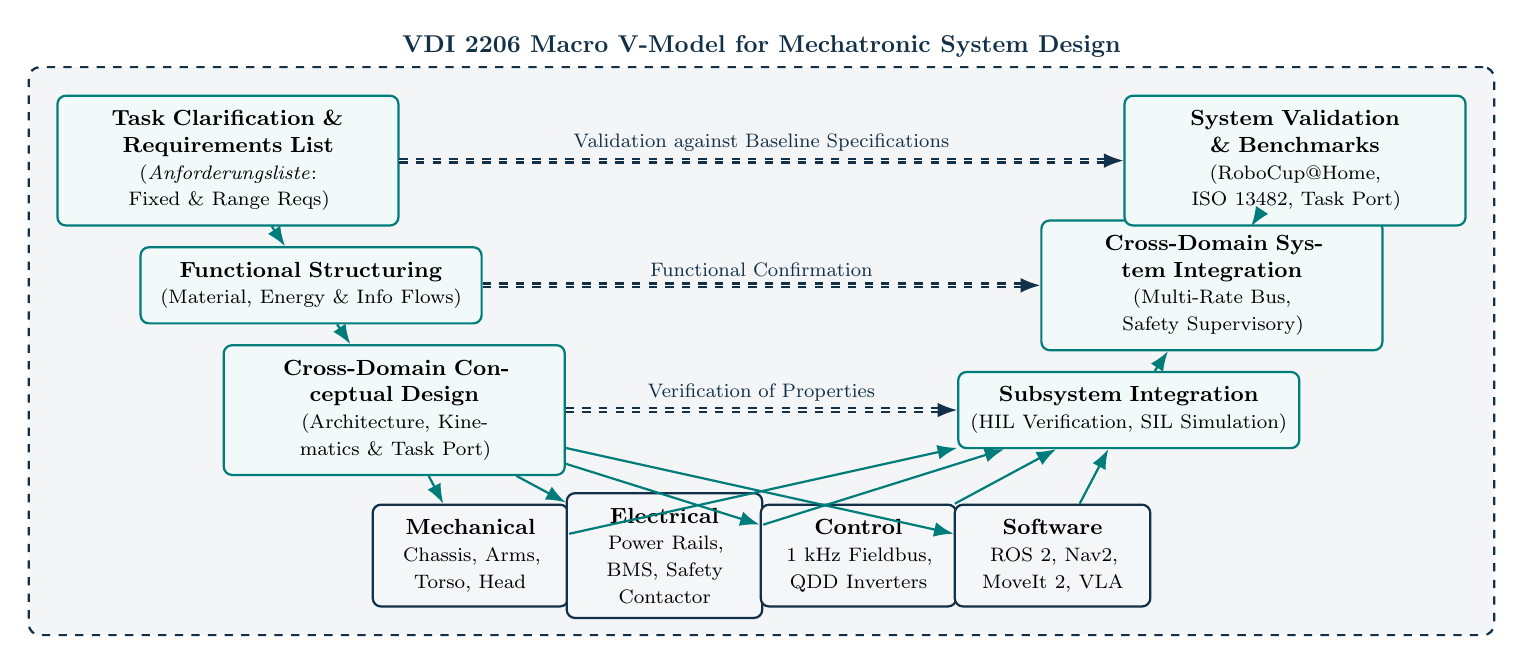
\begin{tikzpicture}[scale=0.88, every node/.style={transform shape}]
  % Macro V-Model Left Side (Top-Down)
  \node[block, text width=4.5cm] (req) at (0, 4.5) {\textbf{Task Clarification \& Requirements List}\\\footnotesize (\emph{Anforderungsliste}: Fixed \& Range Reqs)};
  \node[block, text width=4.5cm] (func) at (1.2, 2.7) {\textbf{Functional Structuring}\\\footnotesize (Material, Energy \& Info Flows)};
  \node[block, text width=4.5cm] (concept) at (2.4, 0.9) {\textbf{Cross-Domain Conceptual Design}\\\footnotesize (Architecture, Kinematics \& Task Port)};

  % Domain Specific Elaboration (Base of V)
  \node[device, text width=2.4cm] (mech) at (3.5, -1.2) {\textbf{Mechanical}\\\footnotesize Chassis, Arms, Torso, Head};
  \node[device, text width=2.4cm] (elec) at (6.3, -1.2) {\textbf{Electrical}\\\footnotesize Power Rails, BMS, Safety Contactor};
  \node[device, text width=2.4cm] (ctrl) at (9.1, -1.2) {\textbf{Control}\\\footnotesize 1~kHz Fieldbus, QDD Inverters};
  \node[device, text width=2.4cm] (soft) at (11.9, -1.2) {\textbf{Software}\\\footnotesize ROS 2, Nav2, MoveIt 2, VLA};

  % Macro V-Model Right Side (Bottom-Up)
  \node[block, text width=4.5cm] (subsys_int) at (13.0, 0.9) {\textbf{Subsystem Integration}\\\footnotesize (HIL Verification, SIL Simulation)};
  \node[block, text width=4.5cm] (sys_int) at (14.2, 2.7) {\textbf{Cross-Domain System Integration}\\\footnotesize (Multi-Rate Bus, Safety Supervisory)};
  \node[block, text width=4.5cm] (valid) at (15.4, 4.5) {\textbf{System Validation \& Benchmarks}\\\footnotesize (RoboCup@Home, ISO 13482, Task Port)};

  % Connecting Arrows of the V
  \draw[arrow] (req) -- (func);
  \draw[arrow] (func) -- (concept);
  \draw[arrow] (concept) -- (mech);
  \draw[arrow] (concept) -- (elec);
  \draw[arrow] (concept) -- (ctrl);
  \draw[arrow] (concept) -- (soft);

  \draw[arrow] (mech) -- (subsys_int);
  \draw[arrow] (elec) -- (subsys_int);
  \draw[arrow] (ctrl) -- (subsys_int);
  \draw[arrow] (soft) -- (subsys_int);
  \draw[arrow] (subsys_int) -- (sys_int);
  \draw[arrow] (sys_int) -- (valid);

  % Verification & Validation Cross-Links
  \draw[bus, dashed] (concept) -- node[above, font=\footnotesize] {Verification of Properties} (subsys_int);
  \draw[bus, dashed] (func) -- node[above, font=\footnotesize] {Functional Confirmation} (sys_int);
  \draw[bus, dashed] (req) -- node[above, font=\footnotesize] {Validation against Baseline Specifications} (valid);

  % Bounding box for V-model
  \begin{scope}[on background layer]
    \node[subsystem, fit=(req) (valid) (mech) (soft), label={[navy, font=\bfseries]above:VDI 2206 Macro V-Model for Mechatronic System Design}] {};
  \end{scope}
\end{tikzpicture}%
}
\caption{The VDI 2206 macro-level V-model adapted for the modular semi-humanoid platform, illustrating the descent from requirements formulation to domain-specific elaboration, followed by ascending multi-stage verification and validation.}
\label{fig:vdi2206_vmodel}
\end{figure}

\subsubsection{The Macro V-Model}
As illustrated in Figure~\ref{fig:vdi2206_vmodel}, the macro V-model coordinates the overall lifecycle across three primary phases:
\begin{enumerate}[leftmargin=1.5em]
  \item \textbf{Left Descending Branch (Specification \& Conceptual Design):} Begins with comprehensive task clarification and drafting a structured requirements list (\emph{Anforderungsliste}), dividing specifications into fixed requirements (\emph{Festforderungen}) and range requirements (\emph{Bereichsforderungen}). These specifications are abstracted into functional structures modeling conserved transport and transformation of \emph{material}, \emph{energy}, and \emph{information}. From these abstractions, cross-domain architectures and kinematics are synthesized.
  \item \textbf{Base of the V-Model (Domain-Specific Concurrent Elaboration):} Development branches concurrently into mechanical structural design (FEA optimization, link geometry, drivetrain selection), electrical hardware design (power architecture, galvanic isolation, BMS), embedded control design (real-time motor commutation, fieldbus deterministic timing), and computer software development (ROS~2 nodes, kinematic solvers, behavior trees).
  \item \textbf{Right Ascending Branch (Integration, Verification, and Validation):} Concurrently developed domain models and physical sub-assemblies are integrated hierarchically. Physical components undergo Software-in-the-Loop (SIL) simulation in high-fidelity physics engines, followed by Hardware-in-the-Loop (HIL) dynamometer testing, full mechatronic integration, and empirical validation against standardized benchmark scenarios.
\end{enumerate}

\subsubsection{The Recurring Problem-Solving Micro-Cycle}
Operating recursively within every macro-phase of the V-model is the 6-stage VDI~2206 problem-solving micro-cycle. This systematic cognitive loop compels the engineering team to validate conceptual variants objectively before freezing interfaces:
\begin{enumerate}[leftmargin=1.5em]
  \item \textbf{Situation Analysis (\emph{Situationsanalyse}):} Rigorous audit of current boundary conditions, state-of-the-art benchmarks (e.g., RoboCup@Home, TIAGo Pro, Reachy 2), physical bottlenecks, and failure modes observed in existing platforms.
  \item \textbf{Goal Formulation (\emph{Zielformulierung}):} Definition of unambiguous, quantitative target criteria (e.g., arm settling time $t_{\text{settling}} \le 0.4\text{ s}$, continuous payload $\ge 2.0\text{ kg}$, footprint $\le 540\text{ mm}$).
  \item \textbf{Solution Synthesis (\emph{Synthese von L{\"o}sungen}):} Generation of multiple divergent morphological concepts without premature design lock-in (e.g., contrasting prismatic elevating torso columns against revolute waist pitch joints).
  \item \textbf{Analysis and Evaluation (\emph{Analyse und Bewertung}):} Quantitative trade-off analysis utilizing multi-criteria decision matrices, kinematic simulation, static/dynamic FEA, and bus latency modeling.
  \item \textbf{Decision (\emph{Entscheidung}):} Selection of the optimal concept based on engineering metrics, manufacturing feasibility, cost, and reliability.
  \item \textbf{Planning (\emph{Planung}):} Structuring detailed work packages, defining physical/logical interface contracts, and scheduling verification milestones for the subsequent development cycle.
\end{enumerate}

\subsection{Core Mechatronic Dynamic Principles}
High-performance mobile manipulation requires an uncompromising focus on structural mechanics and dynamic control bandwidth. Unlike static industrial manipulators anchored to rigid concrete foundations, a mobile manipulator operates atop a movable chassis with finite compliance at the wheel-ground contact interface. Rapid arm accelerations generate reaction forces and moments that can induce body sway, structural vibrations, and end-effector tracking errors.

\subsubsection{Structural Natural Frequency and Resonance}
To guarantee responsive, vibration-free motion during high-speed reaching and trajectory tracking, each actuated mechanical link and joint assembly is modeled to first order as an equivalent spring-mass-damper system. The undamped natural angular frequency $\omega_n$ of the joint assembly is governed by:
\begin{equation}
\omega_n = \sqrt{\frac{K}{M}}
\label{eq:natural_frequency}
\end{equation}
where $K$ represents the aggregate mechanical stiffness of the drivetrain (incorporating gearbox torsional stiffness, bearing rigidity, and structural link flexure in $\text{N}\cdot\text{m/rad}$), and $M$ denotes the effective moving mass or reflected rotational inertia about the joint axis in $\text{kg}\cdot\text{m}^2$.

\subsubsection{Settling Time and Operational Bandwidth}
Following a rapid point-to-point repositioning step command, the settling time $t_{\text{settling}}$ (defined as the duration required for Cartesian oscillations to decay permanently within a specified $2\%$ error band) is approximated by:
\begin{equation}
t_{\text{settling}} \approx \frac{4}{\zeta \omega_n}
\label{eq:settling_time}
\end{equation}
where $\zeta$ represents the effective damping ratio of the closed-loop joint assembly. For critically damped or moderately underdamped systems ($0.65 \le \zeta \le 0.85$), minimizing settling time directly demands maximizing the natural frequency $\omega_n$. Low natural frequencies ($\omega_n < 10\text{ Hz}$) result in prolonged structural ringing, severely throttling closed-loop control gains and slowing autonomous pick-and-place cycles.

\subsubsection{Mass Minimization of Distal Links}
Equation~\eqref{eq:natural_frequency} indicates that maximizing $\omega_n$ requires either increasing stiffness $K$ or decreasing moving inertia $M$. However, adding physical material to increase stiffness $K$ inherently increases mass $M$, often degrading performance.

In articulated serial kinematic chains, the total kinetic energy and reflected inertia at proximal actuators are critically dependent on the spatial distribution of mass. By the parallel axis theorem and manipulator Jacobian inertia transformation, the effective inertia $I_{\text{reflected}, j}$ reflected across joint $j$ due to distal links $i > j$ scales quadratically with link reach:
\begin{equation}
I_{\text{reflected}, j} = \sum_{i=j}^{N} \left( I_i + m_i \mathbf{r}_{j,i}^T \mathbf{r}_{j,i} \right)
\label{eq:reflected_inertia}
\end{equation}
where $m_i$ is the mass of link $i$, $I_i$ is its centroidal inertia tensor, and $\mathbf{r}_{j,i}$ is the position vector from joint axis $j$ to the center of mass of link $i$. 

Consequently, minimizing the mass of distal components (such as wrist pitch/roll mechanisms and end-effector grippers) produces a quadratic-to-cubic reduction in reflected inertia at shoulder and elbow joints. This mass reduction shifts structural resonance well above the operational control bandwidth ($\omega_n \ge 25\text{--}35\text{ Hz}$), suppressing oscillations and permitting aggressive, high-bandwidth closed-loop trajectory tracking.

\subsubsection{Structural Rigidity versus Compliance: The Quasi-Direct Drive Paradigm}
A classical conflict in robotics engineering exists between structural rigidity and mechanical compliance:
\begin{itemize}[leftmargin=1.5em]
  \item \textbf{Rigid Actuation with High-Ratio Reductions ($N > 100:1$):} Utilizes multi-stage planetary or harmonic gearboxes to achieve high static holding torque in compact envelopes. However, reflected rotor inertia scales with the square of the gear ratio ($I_{\text{reflected}} = N^2 I_{\text{rotor}}$), resulting in massive mechanical impedance, extreme friction, non-linear backlash, and zero backdrivability. In collaborative environments, accidental physical collisions impart destructive shock loads directly onto the gear teeth, risking mechanical failure and causing severe human injury.
  \item \textbf{Series Elastic Actuators (SEAs):} Introduce physical springs between the gearbox and the load to measure torque via deflection and provide passive impact absorption. However, the intentional introduction of mechanical compliance drastically limits control bandwidth, introduces low-frequency structural resonances ($\omega_n < 8\text{ Hz}$), and degrades high-speed Cartesian precision.
  \item \textbf{Quasi-Direct Drive (QDD) Solution:} To reconcile these conflicting demands, our platform adopts Quasi-Direct Drive (QDD) actuators across the arm joints. QDD pairs high-torque-density, multi-pole brushless DC outrunner motors with single-stage, low-ratio planetary gearings ($1:6 \le N \le 1:10$). This low transmission ratio preserves ultra-low reflected inertia ($I_{\text{ref}} \sim 36\text{--}100 \times I_{\text{rotor}}$), delivers transparent mechanical backdrivability, absorbs physical impact shocks without gear stripping, and enables direct, high-fidelity joint torque estimation via motor phase current feedback:
  \begin{equation}
  \tau_{\text{joint}} \approx N \cdot K_\tau \cdot I_q
  \label{eq:torque_current}
  \end{equation}
  where $K_\tau$ is the motor torque constant and $I_q$ is the quadrature field-oriented control (FOC) current. This allows the software stack to execute active impedance control, presenting soft, compliant virtual stiffness to human co-workers while maintaining high structural rigidity during autonomous manipulation.
\end{itemize}

\subsection{Core Architectural Philosophy: Separation of Capability from Intent}
The central engineering thesis of this project is the rigorous separation of \emph{capability} (the physical robotic platform) from \emph{intent} (the downstream user application or embodied AI cognitive agent).

Autonomous mobile manipulation robots deployed in service and research settings are overwhelmingly engineered as specialized, single-purpose devices: a rigid arm permanently attached to a custom chassis, driven by monolithic software where high-level task logic is entangled directly with motor PWM drivers and kinematics. When the target task changes, the entire system must be fundamentally redesigned.

\begin{figure}[htbp]
\centering
\begin{tikzpicture}[scale=0.9, every node/.style={transform shape}]
  % Top Layer: Intent
  \node[cloud_node, fill=orange!15, draw=orange, thick, text width=12cm] (intent) at (7, 5.0) {
    \textbf{APPLICATION INTENT LAYER}\\\footnotesize
    Autonomous Task Pipelines \quad|\quad Voice Natural Language Planner (Whisper / LLM) \quad|\quad VLA Foundation Models \quad|\quad Web Teleoperation Dashboard
  };

  % Abstraction Layer: Task Port
  \node[block, fill=teal!20, draw=teal, very thick, text width=12cm] (taskport) at (7, 2.1) {
    \textbf{STANDARDIZED TASK PORT ABSTRACTION LAYER}\\\footnotesize
    Standardized ROS 2 Action Servers, Topics \& Services \quad|\quad Kinematic Feasibility \& Singularity Check \quad|\quad Deterministic Safety Supervisor
  };

  % Bottom Layer: Capability
  \node[subsystem, fill=sky!30, draw=navy, thick, text width=12cm] (platform) at (7, -1.0) {
    \textbf{PLATFORM CAPABILITY LAYER (THE MECHATRONIC SUBSTRATE)}\\\footnotesize
    \begin{tabularx}{\textwidth}{CCCC}
      \textbf{Differential Base} & \textbf{Fixed Mast Torso} & \textbf{Dual 6-DoF Arms + Grippers} & \textbf{Perception Head} \\
      \scriptsize Differential Drive & \scriptsize Rigid Spine Assembly & \scriptsize Bimanual Manipulation & \scriptsize Active Pan-Tilt Gaze \\
      \scriptsize ($SE(2)$ Navigation, 2 DoF) & \scriptsize ($500\text{--}1350\text{ mm}$ Envelope) & \scriptsize (12-DoF Arms + 2-DoF Grippers) & \scriptsize (2-DoF Neck / Stereo Audio)
    \end{tabularx}
  };

  % Side gutters separate command flow from feedback and keep labels clear.
  \draw[bus, orange] (intent.east) -- ++(1.0,0) |- node[pos=0.25, right, font=\scriptsize\bfseries, align=left] {High-level\\intent orders} (taskport.east);
  \draw[bus, teal] (taskport.east) -- ++(1.8,0) |- node[pos=0.25, right, font=\scriptsize\bfseries, align=left] {Safe coordinated\\execution commands} (platform.east);
  \draw[arrow, navy, dashed] (platform.west) -- ++(-1.8,0) |- node[pos=0.25, left, font=\scriptsize\bfseries, align=right] {Telemetry\\and fused state} (taskport.west);
  \draw[arrow, navy, dashed] (taskport.west) -- ++(-1.0,0) |- node[pos=0.25, left, font=\scriptsize\bfseries, align=right] {Completion\\and alarms} (intent.west);
\end{tikzpicture}
\caption{The foundational architectural separation between application intent and platform capability mediated through the standardized Task Port abstraction layer.}
\label{fig:separation_philosophy}
\end{figure}

This project establishes the exact opposite paradigm. The robotic platform is engineered as a general-purpose, modular mechatronic substrate that is completely agnostic to the specific downstream application. What the platform physically possesses---a high-traction differential mobile chassis that navigates collision-free, a rigid structural mast torso maintaining a $500\text{--}1350\text{ mm}$ ergonomic reaching envelope, dual 6-DoF QDD arms with compliant parallel-jaw grippers, and a sensorized 2-DoF pan-tilt head that tracks objects and human dialogue (establishing 18 active DoF total)---remains invariant.

As diagrammed in Figure~\ref{fig:separation_philosophy}, the user or cognitive reasoning agent never accesses low-level joint motor drivers, fieldbus packet frames, or kinematic inversion matrices. Instead, all interaction occurs through a formal, standardized abstraction layer termed the \textbf{Task Port}. The application layer supplies \emph{intent} (e.g., ``Pick up the medication bottle from the kitchen counter and bring it to the dining table''), while the platform orchestrates \emph{capability}---autonomously handling perception, global path planning, collision-free inverse kinematics, multi-rate trajectory interpolation, and active contact safety.

\subsection{Document Objectives and Outline}
This document establishes the comprehensive mechatronic system design, architectural specifications, and engineering allocations for the proposed modular semi-humanoid robot. The remainder of this report is organized as follows:
\begin{itemize}[leftmargin=1.5em]
  \item Section~\ref{sec:tasks_benchmarks} grounds platform capabilities in empirical service robotics benchmarks (RoboCup@Home, World Robot Summit, ISO~13482), extracts architectural boundary constraints, conducts morphological benchmarking against contemporary platforms, and defines concrete validation tasks.
  \item Section~\ref{sec:requirements} establishes the formal engineering requirements list (\emph{Anforderungsliste}) classifying constraints across geometry, kinematics, dynamics, electrical power, embedded control, and software.
  \item Section~\ref{sec:functional_structure} details the formal functional structure through conserved material, energy, and information flow models.
  \item Section~\ref{sec:system_architecture} delineates the multi-tier system architecture, real-time communication fieldbuses, safety supervisor, and the Task Port API.
  \item Section~\ref{sec:subsystems_detail} executes device-level deep dives into each functional mechatronic subsystem (mobile base, torso, arms, head, HMI, and power).
  \item Section~\ref{sec:domain_allocation} allocates multidisciplinary engineering tasks across mechanical, electrical, embedded firmware, and software domains.
  \item Section~\ref{sec:bom_roadmap} details the preliminary Bill of Materials (BOM), budget allocation, and phased development roadmap.
  \item Section~\ref{sec:conclusion} synthesizes key mechatronic architectural takeaways and establishes next steps toward physical embodiment and testing.
\end{itemize}

\section{Empirical Task Formulation and Benchmark Derivation}
\label{sec:tasks_benchmarks}

\subsection{Grounding Operational Objectives in Standardized Robotics Benchmarks}
Engineering a general-purpose robotic platform requires establishing operational targets that reflect the physical and cognitive challenges of real-world deployment. In academic literature, robotics projects frequently falter by engineering custom mechanisms tailored to arbitrary, isolated laboratory tasks (e.g., grasping a single specific cylinder on an uncluttered bench). When transferred to unconstrained human environments, such bespoke systems fail due to inadequate kinematic workspace, insufficient payload margins, rigid actuation, or brittle perceptual assumptions.

To ground the platform's functional specifications in validated real-world requirements, this project derives its operational primitives from international competitive service robotics leagues and certified industrial safety standards. These benchmarks capture the environmental variability, clutter, geometric diversity, and dynamic human interactions inherent to human-inhabited spaces.

\subsubsection{The RoboCup@Home Benchmark Suite}
The international RoboCup@Home competition represents the premier global benchmark for autonomous service and domestic robotics~\cite{robocupathome}. Spanning the Domestic Standard Platform League (DSPL), Open Platform League (OPL), and Social Standard Platform League (SSPL), RoboCup@Home assesses mobile manipulators within realistic, fully furnished domestic apartments and office environments. Analyzing rulebooks, technical challenge papers, and operational logs reveals four canonical benchmark tasks that establish the minimum functional envelope of our platform:

\begin{enumerate}[leftmargin=1.5em]
  \item \textbf{General Purpose Service Robot (GPSR):} The GPSR benchmark assesses physical and cognitive generalization without prior environment tuning. High-level commands are generated dynamically via formal grammar engines, categorised into three escalating complexity tiers:
  \begin{itemize}[leftmargin=1.2em]
    \item \emph{Category I (Fully Specified Tasks):} The command explicitly states the required action sequence, target object, and destination (e.g., ``Navigate to the dining table, grasp the green soda can, and place it into the waste basket''). This tier benchmarks deterministic pipeline execution: autonomous Simultaneous Localization and Mapping (SLAM), 3D point-cloud object segmentation, inverse kinematic reachability, and grasp execution.
    \item \emph{Category II (Contextual Tasks):} The command contains ambiguous or missing spatial or semantic information (e.g., ``Bring me a beverage from the kitchen''). The platform must perform semantic spatial reasoning, inspect candidate storage locations across multiple shelf tiers ($300\text{--}1350\text{ mm}$), and initiate spoken clarification dialogue through speech synthesis and directional microphone arrays.
    \item \emph{Category III (Erroneous and Contradictory Tasks):} The command involves physical impossibilities, missing items, or obstructed paths (e.g., requesting an item not present in the room). The robot must verify scene state discrepancies, detect tactile or visual grasp failures, abort hazardous actions safely, verbally articulate the failure mode to human users, and execute fallback behaviors.
  \end{itemize}
  
  \item \textbf{Clean Up and Table Clearing Benchmark:} This task formalizes physical environment rearrangement over the special Euclidean group $SE(3) = \mathbb{R}^3 \times SO(3)$. The autonomous agent must transform an unorganized environment from an initial state $s_0 \in \mathcal{S}$ to a desired tidy configuration $s^* \in \mathcal{S}$ through direct physical contact. The robot must approach standard dining surfaces, segment cluttered tableware (cups, ceramic bowls, silverware, beverage bottles), estimate surface normals, and execute multi-angle grasps without toppling adjacent fragile objects. Furthermore, clearing tableware requires transporting items and placing them into confined dishwasher racks or designated storage bins.
  
  \item \textbf{Interaction with Articulated Domestic Fixtures:} Service environments demand interaction with kinematically constrained fixtures. The robot must approach, unlatch, open, and close hinged cupboard doors, sliding drawers, and spring-loaded refrigerator doors. These operations impose closed kinematic chain constraints where the end-effector trajectory $\mathbf{x}_{\text{EE}}(t)$ is constrained along a 1-DoF circular arc or prismatic rail, requiring compliant contact force regulation ($F_{\text{contact}} \le 30\text{--}50\text{ N}$) to prevent excessive internal stresses.
  
  \item \textbf{Receptionist, Person Following, and Physical Object Handover:} This benchmark evaluates social co-presence and continuous physical human-robot interaction (pHRI). The platform must detect human poses, identify unfamiliar individuals, maintain continuous visual tracking during guided navigation ($v_{\text{walk}} \le 1.2\text{ m/s}$), and preserve proxemic personal zones ($0.8\text{--}1.5\text{ m}$). During physical handovers (delivering a beverage or taking a carry bag), the robot must dynamically adjust arm trajectory to the human hand pose, detect contact via wrist force-torque sensing or motor current monitoring, and execute smooth, intentional payload releases at safe approach velocities ($v_{\text{EE}} \le 0.3\text{ m/s}$).
\end{enumerate}

\subsubsection{World Robot Summit (WRS) Partner Robot Challenge}
The World Robot Summit (WRS) Partner Robot Challenge~\cite{wrs} provides complementary empirical validation protocols centered on daily life assistance in standard living spaces. The WRS benchmark emphasizes:
\begin{itemize}[leftmargin=1.5em]
  \item \textbf{Tidy-Up Operations in Cluttered Living Rooms:} Retrieval of deformable objects (clothing, blankets), thin items lying flat on the floor (pens, paper sheets), and small accessories stored inside low drawers ($200\text{--}400\text{ mm}$ height).
  \item \textbf{Continuous Execution Autonomy:} Penalizing teleoperation interventions and rewarding continuous, uninterrupted multi-step task execution over extended time horizons ($15\text{--}30\text{ minutes}$).
  \item \textbf{Strict Safety Penalties:} Automatic disqualification or severe scoring deductions for collisions with furniture walls exceeding dynamic impact thresholds ($>20\text{ N}$).
\end{itemize}

\subsubsection{Safety Certification Standards: ISO 13482:2014}
Deploying mobile manipulators in human-inhabited environments requires rigorous adherence to safety standards. The platform is engineered to comply with \textbf{ISO~13482:2014} (``Robots and robotic devices --- Safety requirements for personal care robots'')~\cite{iso13482}, under the classification of a \emph{mobile servant robot}. Key mandates governing the mechatronic design include:
\begin{itemize}[leftmargin=1.5em]
  \item \textbf{Hazard Mitigation and Risk Reduction:} Systematic elimination of mechanical pinch and shear points at articulated arm joints, torso elevation columns, and wheel cowlings.
  \item \textbf{Emergency Stop and Operational Interlocks:} Integration of a Category~3, Performance Level~d (PL~d) dual-channel safety circuit capable of de-energizing all actuator drive inverters within $t_{\text{stop}} \le 10\text{ ms}$ upon E-stop actuation or safety LiDAR field breach.
  \item \textbf{Limitation of Contact Forces and Speed:} Adherence to collaborative power and force limiting principles (incorporating ISO/TS 15066 guidelines), ensuring transient impact forces remain below human pain thresholds ($F_{\text{impact}} \le 150\text{ N}$, quasi-static crushing force $F_{\text{crush}} \le 50\text{--}75\text{ N}$), supported by backdrivable Quasi-Direct Drive (QDD) actuators and soft-skinned compliant end effectors.
  \item \textbf{Overturning Stability:} Maintaining static and dynamic stability under maximum arm reach ($R_{\text{arm}} \approx 750\text{ mm}$), maximum continuous payload ($m_{\text{load}} = 3.0\text{ kg}$ per arm), and maximum base deceleration ($a_{\text{base}} = 1.0\text{ m/s}^2$).
\end{itemize}

\begin{table}[htbp]
\centering\small
\caption{Systematic derivation of mechatronic primitives and physical constraints from empirical benchmarks.}
\label{tab:benchmark_mapping}
\begin{tabularx}{\textwidth}{@{}lYYY@{}}
\toprule
\textbf{Benchmark Source} & \textbf{Operational Sub-Tasks} & \textbf{Underlying Mechatronic Primitives} & \textbf{Physical \& Environmental Constraints} \\
\midrule
RoboCup@Home GPSR (Cat.~I)~\cite{robocupathome} & Autonomous pick-and-place, point-to-point transit, object sorting & Holonomic SLAM navigation, 3D point-cloud registration, $SE(3)$ trajectory generation, parallel grasp & Doorway width $\ge 750\text{ mm}$; table height $720\text{--}750\text{ mm}$; item mass $\le 1.5\text{ kg}$ \\
\addlinespace[0.4em]
RoboCup@Home GPSR (Cat.~II)~\cite{robocupathome} & Contextual item retrieval, dialogue clarification, shelf search & Directional audio parsing (STT), semantic mapping, active pan-tilt visual search, multi-height reach & Ambient acoustic noise $50\text{--}65\text{ dB}$; multi-tier shelf search ($300\text{--}1350\text{ mm}$) \\
\addlinespace[0.4em]
RoboCup@Home GPSR (Cat.~III)~\cite{robocupathome} & Discrepancy detection, grasp slip detection, safety abort & Proprioceptive current monitoring, wrist F/T tactile sensing, speech synthesis (TTS), exception recovery & Dynamic human obstacles; safe deceleration $a_{\text{dec}} \le 1.0\text{ m/s}^2$; timeout $\le 5\text{ min}$ \\
\addlinespace[0.4em]
Clean Up \& Table Clearing~\cite{robocupathome} & Tableware segmentation, dishwasher loading, surface clearing & Dense RGB-D normal estimation, compliant grasp closure, high-accuracy Cartesian positioning ($\le \pm 2\text{ mm}$) & Fragile ceramic/glass targets; grasp span $20\text{--}90\text{ mm}$; vertical clearance $\le 350\text{ mm}$ \\
\addlinespace[0.4em]
WRS Partner Robot~\cite{wrs} & Tidy-up from floor, articulated drawer/door opening & Ground-level reaching ($z = 0\text{ mm}$), constrained circular/prismatic path following, impedance control & Floor-level grasping; pulling forces up to $40\text{ N}$; zero wall collision damage \\
\addlinespace[0.4em]
Receptionist \& Handover~\cite{robocupathome} & Person following, proxemic navigation, compliant physical handover & 2D/3D human skeletal tracking, dynamic costmap avoidance, soft wrist impedance, release timing & Human walking speed $\le 1.2\text{ m/s}$; social distance $0.8\text{--}1.5\text{ m}$; handover speed $\le 0.3\text{ m/s}$ \\
\addlinespace[0.4em]
ISO 13482 Compliance~\cite{iso13482} & Safe co-presence, emergency stop, physical impact limitation & Dual-channel hardware E-stop, software safety supervisory monitor, backdrivable QDD actuation & Safety cutoff $t_{\text{stop}} \le 10\text{ ms}$; impact force $F \le 150\text{ N}$; crushing force $\le 50\text{ N}$ \\
\bottomrule
\end{tabularx}
\end{table}

\subsection{Physical Boundary Conditions and Kinematic Sizing}
Synthesizing the empirical requirements from Table~\ref{tab:benchmark_mapping} directly dictates the geometric envelope and kinematic reach of the semi-humanoid platform:

\begin{itemize}[leftmargin=1.5em]
  \item \textbf{Doorway Clearances and Base Footprint:} Standard residential and commercial interior doorways exhibit clear aperture widths between $750\text{ mm}$ and $900\text{ mm}$. To guarantee safe, collision-free transit with an adequate lateral clearance margin ($\ge 75\text{--}100\text{ mm}$ per side), the maximum mobile base footprint diameter is constrained to:
  \begin{equation}
  D_{\text{base}} \le 540\text{--}600\text{ mm}
  \end{equation}
  
  \item \textbf{Vertical Workspace Envelope:} Standard architectural furnishings exhibit strictly standardized working heights:
  \begin{itemize}
    \item \emph{Floor Level ($z = 0\text{ mm}$):} Fallen objects, shoes, floor tidy-up.
    \item \emph{Dining Tables and Desks ($z = 720\text{--}750\text{ mm}$):} Standard meal surfaces and workstations.
    \item \emph{Kitchen Counters and Workbenches ($z = 850\text{--}900\text{ mm}$):} Food preparation, appliance manipulation.
    \item \emph{Intermediate and High Shelves ($z = 1000\text{--}1350\text{ mm}$):} Cupboards, pantry shelves, wall cabinets.
  \end{itemize}
  By establishing the shoulder yoke at an ergonomic height of $\approx 950\text{ mm}$ on a rigid structural mast, the dual 6-DoF manipulators cover a continuous vertical manipulation reach band from $500\text{ mm}$ to $1350\text{ mm}$. This directly spans dining tables ($750\text{ mm}$), kitchen counters ($900\text{ mm}$), and eye-level shelves purely through joint articulation, avoiding the parasitic dead weight, mechanical binding risk, and cost of an active prismatic mast in the baseline build (while supporting an optional modular telescopic column for extended floor-to-ceiling reach).
  
  \item \textbf{Continuous Payload Demands:} Everyday domestic and laboratory objects (beverage mugs, full 1.5-liter water bottles, books, canned goods, medical supply kits) weigh between $0.2\text{ kg}$ and $2.0\text{ kg}$. To maintain a safety margin of $1.5\times$ during dynamic accelerations ($a_{\text{EE}} \approx 1.5\text{ m/s}^2$), each manipulator must provide a continuous payload rating:
  \begin{equation}
  m_{\text{payload}} \ge 2.0\text{ kg} \quad (\text{nominal target: } 3.0\text{ kg per arm})
  \end{equation}
\end{itemize}

\subsection{Morphological Benchmarking of Contemporary Mobile Manipulators}
To contextualize the mechatronic design within state-of-the-art robotics engineering, Table~\ref{tab:robot_comparison} details a rigorous comparative analysis across five prominent mobile manipulation platforms: PAL Robotics TIAGo Pro~\cite{tiagopro}, Pollen Robotics Reachy~2~\cite{reachy2}, Stanford/AgileX Mobile ALOHA~\cite{mobilealoha}, Menlo Research Asimov~1~\cite{asimov1}, and Hello Robot Stretch~3~\cite{stretch}.

\begin{table}[htbp]
\centering\scriptsize
\caption{Comprehensive morphological and mechatronic benchmarking of leading mobile manipulation systems.}
\label{tab:robot_comparison}
\begin{tabularx}{\textwidth}{@{}lYYYYYY@{}}
\toprule
\textbf{Specification Parameter} & \textbf{PAL Robotics TIAGo Pro}~\cite{tiagopro} & \textbf{Pollen Robotics Reachy 2}~\cite{reachy2} & \textbf{Mobile ALOHA (AgileX)}~\cite{mobilealoha} & \textbf{Menlo Research Asimov 1}~\cite{asimov1} & \textbf{Hello Robot Stretch 3}~\cite{stretch} & \textbf{Proposed Platform} \\
\midrule
\textbf{Morphology Category} & Modular Semi-Humanoid (Wheeled AMR) & An\-thro\-po\-mor\-phic Upper Body (Wheeled opt.) & Bimanual Mobile Manipulator & Bipedal Humanoid (Upper Body relevant) & Minimalist Prismatic Mobile Manipulator & Modular General-Purpose Semi-Humanoid \\
\addlinespace[0.2em]
\textbf{Total Actuated DoF} & 23 DoF (Base: 2-3, Torso: 1, Arms: $2 \times 7$, Head: 2, Grip: 2) & 21--23 DoF (Arms: $2 \times 7$, Grip: 2, Head: 3, Antennas: 2) & 16 DoF (Base: 2, Arms: $2 \times 6$, Grippers: 2) & 25 DoF (Legs: $2 \times 6$, Waist: 1, Arms: $2 \times 5$, Head: 2) & 5 DoF (Base: 2, Mast Lift: 1, Arm Telescoping: 1, Grip: 1) & 18 DoF (Base: 2, Arms: $2 \times 6$, Grip: 2, Head: 2) \\
\addlinespace[0.2em]
\textbf{Continuous Arm Payload} & 3.0~kg per arm (excluding gripper) & 3.0~kg per arm & 0.75~kg (ViperX) to 1.5~kg (PiPER) & $\sim 1.5$~kg per arm & 1.5~kg (at full horizontal extension) & 2.0--3.0~kg per arm \\
\addlinespace[0.2em]
\textbf{Manipulator Reach} & Vertical: 920--960~mm; Horiz. span: 2360~mm & Full arm span $\sim 1400$~mm & Vertical: 650--2000~mm; Horiz: 1000~mm & Arm reach $\sim 600$~mm; waist yaw rotation & Vertical: 1100~mm; Horiz. stroke: 520~mm & Vertical: 500--1350~mm; Horiz. reach: 625~mm \\
\addlinespace[0.2em]
\textbf{Torso / Lift Stroke} & Active telescopic column: 350~mm stroke & Fixed an\-thro\-po\-mor\-phic chest & Fixed extrusion frame; static height & Fixed torso frame with 1-DoF waist yaw & Vertical carriage on fixed mast ($1100\text{ mm}$) & Fixed structural mast (optional column: 300~mm) \\
\addlinespace[0.2em]
\textbf{Base Drive Kinematics} & Differential ($\varnothing 540\text{ mm}$) or Mecanum ($710 \times 490\text{ mm}$) & Om\-ni\-di\-rec\-tion\-al wheeled base (optional) & Differential drive (AgileX Tracer AGV) & Bipedal dynamic walking legs (6-DoF/leg) & Differential drive (dual central wheels + castors) & Differential drive (2 active wheels + 2 casters) \\
\addlinespace[0.2em]
\textbf{Max Base Velocity} & 1.0~m/s & 0.8--1.0~m/s & 1.5--2.0~m/s & 0.8--1.2~m/s (walking) & 0.6~m/s & 0.8--1.0~m/s \\
\addlinespace[0.2em]
\textbf{Total System Mass} & 60--72~kg (diff), 95~kg (omni) & $\sim 35\text{--}40\text{ kg}$ (upper body + base) & $\sim 75\text{ kg}$ (with battery bank \& arms) & 35~kg & 24.5~kg & $\sim 45\text{--}50\text{ kg}$ (statically balanced) \\
\addlinespace[0.2em]
\textbf{Actuator Technology} & Series Elastic Actuators (SEAs) + torque sensors & Custom Orbita 2D/3D spherical modules & Off-the-shelf industrial servos (Dynamixel) & BLDC motors + low-ratio planetary (QDD) & Stepper motors + belt drives + compliance springs & Tiered Hybrid: QDD (proximal) + Bus Servos (distal) \\
\addlinespace[0.2em]
\textbf{Internal Fieldbus} & Real-time EtherCAT (1~kHz closed loop) & CAN bus + USB 3.0 / Serial & CAN bus (arms \& base) & 5$\times$ CAN @ 1~Mbps + 1$\times$ CAN @ 500~kbps & USB over internal serial UART & 1~Mbps CAN 2.0B / TWAI + 1~Mbps Half-Duplex TTL \\
\addlinespace[0.2em]
\textbf{Battery Chemistry \& Life} & 36V 20Ah Li-ion (8--10~h runtime) & 24V--48V Li-ion (4--6~h runtime) & 24V 30Ah LFP base + 1024Wh pack (12~h) & 48V Li-ion pack ($\sim 1\text{--}2\text{ h}$ walking) & 12V 20Ah LiFePO4 ($\sim 4\text{ h}$) & 24V 20Ah LiFePO4 ($\sim 480\text{ Wh}$, $\sim 3.5\text{ h}$) \\
\addlinespace[0.2em]
\textbf{Compute Architecture} & Intel Core i7 + NVIDIA Jetson GPU & Industrial x86 SBC + NVIDIA Jetson Orin & Onboard laptop (Intel i7 + RTX GPU) & Radxa CM5 (motion) + Raspberry Pi 5 & Intel Core i5 embedded computer & Jetson Orin NX 16GB + 5$\times$ ESP32 MCUs \\
\bottomrule
\end{tabularx}
\end{table}

\subsubsection{Mechatronic Design Trade-Off Analysis}
Evaluating the comparative architectural implementations in Table~\ref{tab:robot_comparison} highlights three decisive mechatronic trade-offs that govern our design synthesis:

\begin{enumerate}[leftmargin=1.5em]
  \item \textbf{Torso Architecture: Fixed Structural Mast versus Prismatic Lift Column:}
  While active prismatic lift columns (e.g., TIAGo Pro) extend vertical stroke down to floor level, they introduce severe structural liabilities. When dual arms carrying payloads extend forward, the resulting cantilever moment ($M_{\text{cant}} = \sum m_i g L_i$) induces extreme normal reaction forces across linear bearing carriages, causing mechanical binding, stick-slip wear, and motor current surges. Furthermore, a motorized prismatic stage adds $10\text{--}15\text{ kg}$ of parasitic dead mass that elevates the center of mass ($z_{\text{CoM}}$) and increases tipping risk.
  
  Our design implements a rigid 6061-T6 aluminum extrusion mast with shoulder height at $\approx 950\text{ mm}$. The dual 6-DoF manipulators cover a continuous vertical manipulation envelope from $500\text{ mm}$ to $1350\text{ mm}$ purely through joint kinematics, directly covering standard dining tables ($750\text{ mm}$), countertops ($900\text{ mm}$), and eye-level shelves without moving torso pinch hazards, while lowering $z_{\text{CoM}} \le 350\text{ mm}$. The telescopic column is maintained as a modular, bolt-on upgrade (+EGP 32,920) rather than a baseline requirement.

  \item \textbf{Base Drivetrain: High-Traction Differential Drive versus Omnidirectional Mecanum Drive:}
  While omnidirectional Mecanum wheel drives provide instantaneous 3-DoF planar velocity control ($\dot{x}, \dot{y}, \dot{\theta}$), their angled peripheral rollers suffer from $15\text{--}20\%$ non-linear wheel slip on domestic floors, leading to rapid dead-reckoning drift in wheel odometry. Furthermore, Mecanum rollers generate severe high-frequency chassis vibrations on hard floors, struggle with carpet pile friction, and are prone to jamming from domestic debris (hairs, fibers).
  
  In contrast, a differential drive topology with two large $\varnothing 200\text{ mm}$ vulcanized rubber wheels and two passive $100\text{ mm}$ swivel casters provides superior traction ($\mu_s \ge 0.85$), smooth and quiet rolling, flawless threshold traversal ($15\text{--}20\text{ mm}$ height), zero-radius turning on the spot ($R_{\text{turn}} = 0$), and highly deterministic odometric tracking.

  \item \textbf{Actuator Paradigm: Tiered Hybrid QDD and Bus Servos versus All-Harmonic Arms:}
  Conventional collaborative arms utilizing all-harmonic drivetrains (e.g., Franka Panda, UR3) achieve high static precision but suffer from high gear ratios ($N > 100:1$), enormous reflected inertia ($I_{\text{ref}} = N^2 I_{\text{rotor}} > 10{,}000 I_{\text{rotor}}$), non-backdrivability, and prohibitive cost ($>\$25{,}000$). Conversely, hobby-grade multi-servo arms fail under continuous payload holding torques.
  
  Our design introduces a tiered hybrid actuation architecture: high-torque CubeMars AK70-10 QDD modules ($24.8\text{ N}\cdot\text{m}$, $10:1$ planetary ratio) power high-load proximal joints (shoulder pitch/roll/yaw, elbow pitch), providing transparent backdrivability, impact tolerance, and direct phase-current torque estimation. Distal wrist joints (pitch, roll) and parallel-jaw grippers deploy lightweight Feetech STS3215/STS3032 serial bus servos, cutting distal mass by nearly $90\%$, lowering reflected inertia quadratically, and drastically reducing arm cost to EGP~190,550 for both arms.
\end{enumerate}

\subsection{Definition of Concrete Platform Validation Benchmarks}
To empirically validate the core design philosophy---specifically proving that the mechatronic platform exposes a complete, robust set of operational capabilities that can be commanded exclusively through the standardized Task Port without modifying underlying control loops---this project defines two concrete validation benchmarks.

\subsubsection{Benchmark 1: Primary Proof-of-Concept Task --- Autonomous Voice-Commanded Pick-and-Place}
The primary benchmark represents an end-to-end autonomous mobile manipulation workflow commanded entirely via unconstrained spoken natural language. This benchmark validates the multi-layer integration of acoustic perception, cognitive task planning, Task Port API decoupling, autonomous navigation, and compliant grasping.

\begin{figure}[htbp]
\centering
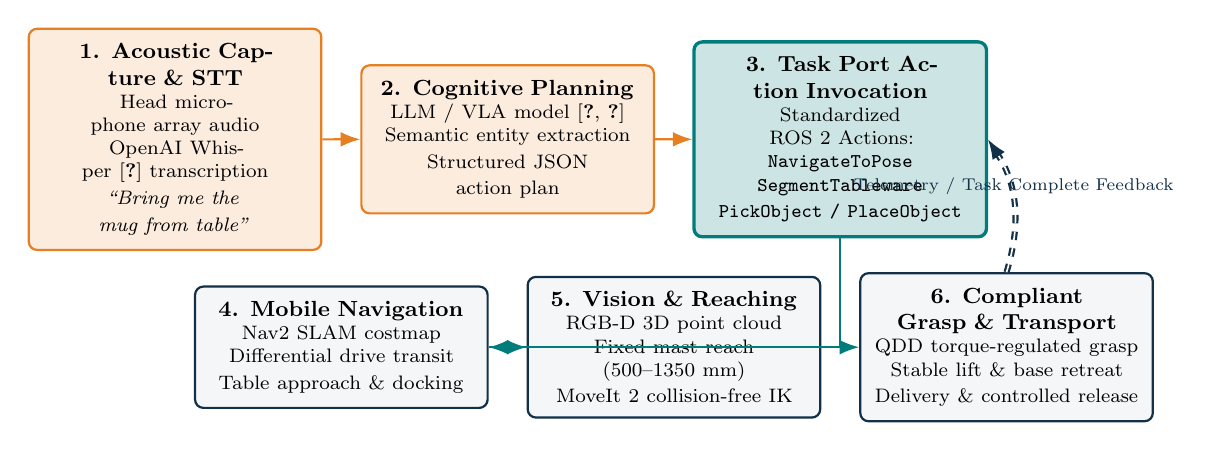
\begin{tikzpicture}[scale=0.88, every node/.style={transform shape}]
  % Pipeline nodes
  \node[block, fill=orange!15, draw=orange, text width=3.8cm] (voice) at (0, 3.0) {
    \textbf{1. Acoustic Capture \& STT}\\\footnotesize
    Head microphone array audio\\
    OpenAI Whisper~\cite{whisper} transcription\\
    \emph{``Bring me the mug from table''}
  };

  \node[block, fill=orange!15, draw=orange, text width=3.8cm] (planner) at (4.8, 3.0) {
    \textbf{2. Cognitive Planning}\\\footnotesize
    LLM / VLA model~\cite{openvla,rtx}\\
    Semantic entity extraction\\
    Structured JSON action plan
  };

  \node[block, fill=teal!20, draw=teal, very thick, text width=3.8cm] (taskport_node) at (9.6, 3.0) {
    \textbf{3. Task Port Action Invocation}\\\footnotesize
    Standardized ROS 2 Actions:\\
    \texttt{NavigateToPose}\\
    \texttt{SegmentTableware}\\
    \texttt{PickObject / PlaceObject}
  };

  \node[device, text width=3.8cm] (nav) at (2.4, 0.0) {
    \textbf{4. Mobile Navigation}\\\footnotesize
    Nav2 SLAM costmap\\
    Differential drive transit\\
    Table approach \& docking
  };

  \node[device, text width=3.8cm] (perc) at (7.2, 0.0) {
    \textbf{5. Vision \& Reaching}\\\footnotesize
    RGB-D 3D point cloud\\
    Fixed mast reach ($500\text{--}1350\text{ mm}$)\\
    MoveIt 2 collision-free IK
  };

  \node[device, text width=3.8cm] (manip) at (12.0, 0.0) {
    \textbf{6. Compliant Grasp \& Transport}\\\footnotesize
    QDD torque-regulated grasp\\
    Stable lift \& base retreat\\
    Delivery \& controlled release
  };

  % Connecting arrows
  \draw[arrow, orange] (voice) -- (planner);
  \draw[arrow, orange] (planner) -- (taskport_node);
  \draw[arrow, teal] (taskport_node) |- (nav);
  \draw[arrow, teal] (nav) -- (perc);
  \draw[arrow, teal] (perc) -- (manip);

  % Feedback
  \draw[bus, navy, dashed] (manip.north) to[bend right=25] node[above, font=\scriptsize] {Telemetry / Task Complete Feedback} (taskport_node.east);
\end{tikzpicture}
\caption{End-to-end execution pipeline for Validation Benchmark 1: Autonomous voice-commanded pick-and-place mediated strictly across the Task Port interface.}
\label{fig:benchmark1_pipeline}
\end{figure}

As diagrammed in Figure~\ref{fig:benchmark1_pipeline}, the execution pipeline progresses as follows:
\begin{enumerate}[leftmargin=1.5em]
  \item \textbf{Acoustic Capture and Speech Recognition:} Ambient audio is captured via the head-mounted directional microphone array and processed locally or edge-hosted by OpenAI Whisper~\cite{whisper}. Whisper translates the acoustic waveform into a normalized text transcript:
  \begin{equation}
  \mathbf{w}_{\text{audio}} \xrightarrow{\text{Whisper STT}} \mathbf{s}_{\text{text}} = \text{``Fetch the green mug and place it on the table.''}
  \end{equation}
  
  \item \textbf{Cognitive Intent Parsing and Plan Decomposition:} A cognitive Large Language Model (LLM) or Vision-Language-Action (VLA) foundation planner (e.g., OpenVLA~\cite{openvla}, RT-X~\cite{rtx}) interprets the transcript, resolves semantic spatial references against a topological semantic map of the arena, and decomposes the high-level intent into a structured sequence of discrete Task Port action goals:
  \begin{equation}
  \Pi = \left\{ \text{Nav}(\text{counter}), \text{Perceive}(\text{``green mug''}), \text{Grasp}(\mathbf{T}_{\text{grasp}}), \text{Nav}(\text{table}), \text{Place}(\mathbf{T}_{\text{place}}) \right\}
  \end{equation}

  \item \textbf{Task Port Invocation and Autonomous Execution:} The task client script interacts \emph{exclusively} through the Task Port API:
  \begin{itemize}
    \item Invoking \texttt{NavigateToPose}$(x, y, \theta)$ triggers Nav2, driving the differential chassis to the target pose while avoiding obstacles.
    \item \emph{Workspace Matching:} The fixed structural mast positions the shoulder yoke at $\approx 950\text{ mm}$, placing the countertop natively within the $500\text{--}1350\text{ mm}$ arm reaching envelope without requiring auxiliary prismatic lift motion.
    \item Invoking \texttt{PerceiveTarget}(``green mug'') commands the pan-tilt head camera to localize the target, returning an estimated $SE(3)$ grasp pose $\mathbf{T}_{\text{grasp}}$ and surface normal vector $\mathbf{n}$.
    \item Invoking \texttt{ExecuteBimanualPick}($\mathbf{T}_{\text{grasp}}$) triggers MoveIt~2 collision-free trajectory planning and QDD current-regulated grasp closure ($F_{\text{normal}} \approx 15\text{ N}$).
    \item The platform navigates to the destination surface, confirms clearance via depth sensing, and gently places the payload under controlled deceleration.
  \end{itemize}
  
  \item \textbf{Validation Metric:} Successful autonomous task completion across 10 consecutive trials without manual operator intervention, maintaining positional repeatability $\le \pm 2.0\text{ mm}$, zero collision events, and execution latency under $120\text{ seconds}$.
\end{enumerate}

\subsubsection{Benchmark 2: Secondary Task --- Interactive Web Dashboard Teleoperation, Alarm Monitoring, and Task Programming}
The secondary benchmark validates the platform's Human-Machine Interface (HMI), real-time operational observability, diagnostic safety mechanisms, and no-code task programming capability:

\begin{enumerate}[leftmargin=1.5em]
  \item \textbf{Low-Latency Interactive Teleoperation:} Validation of supervisory manual control through a browser-based WebRTC/WebSocket dashboard. The operator exercises decoupled velocity jogging of the differential base ($v_x, \omega_z$ via virtual joystick) and Cartesian 6-DoF end-effector jogging of dual arms. Video feeds from the stereo perception head and wrist cameras stream at $1080\text{p} @ 30\text{ fps}$ with end-to-end network latency $t_{\text{latency}} \le 80\text{ ms}$ over local Wi-Fi~6.
  
  \item \textbf{Real-Time Telemetry and Multi-Level Alarm Monitoring:} Continuous telemetry aggregation streaming from embedded controllers to the HMI:
  \begin{itemize}
    \item Battery Management System (BMS) health: cell voltage balance, State of Charge (SoC), pack temperature, and discharge current.
    \item Actuator drive diagnostics: motor winding temperatures, FOC inverter phase currents, bus voltage sag, and fieldbus cyclic jitter ($<50\text{ }\mu\text{s}$).
    \item Live safety interlock supervision: monitoring safety LiDAR zone infringements, physical E-stop contactor status, and torque-limit exceedance alarms.
  \end{itemize}
  
  \item \textbf{Interactive Waypoint-Based Task Programming (Record-and-Replay):} To empower non-expert operators to program tasks without writing code, the dashboard provides a graphical record-and-replay interface:
  \begin{itemize}
    \item The operator backdrives the compliant QDD arms manually (kinesthetic teaching) or jogs the robot to key spatial waypoints.
    \item Waypoints are logged as timestamped $SE(3)$ end-effector poses and base coordinates:
    \begin{equation}
    \mathcal{W}_k = \left\{ \mathbf{T}_{\text{base}, k}, \mathbf{T}_{\text{left}, k}, \mathbf{T}_{\text{right}, k}, g_{\text{left}, k}, g_{\text{right}, k} \right\}
    \end{equation}
    \item The interface constructs a graphical Behavior Tree or linear motion script, parameterizing velocities, blend radii, and grasp thresholds.
    \item The generated task is flashed directly through the Task Port API, where the platform autonomously synthesizes smooth quintic polynomial trajectories between waypoints and executes the sequence repeatably.
  \end{itemize}

  \item \textbf{Validation Metric:} Rapid programming ($<10\text{ minutes}$) and verified autonomous replay of a multi-waypoint tray-clearing routine, with live diagnostic alarms correctly flagging simulated fault conditions (e.g., motor thermal warning at $75^\circ\text{C}$ or artificial path obstruction) and bringing the platform to a controlled stop.
\end{enumerate}

\section{Engineering Requirements Specification}
\label{sec:requirements}

\subsection{Formal Requirements Classification under VDI 2206}
The task clarification and conceptual design of complex mechatronic systems must proceed from a structured, unambiguous specification of engineering requirements. In accordance with the VDI~2206 design guideline (\emph{Entwicklungsmethodik f{\"u}r mechatronische und cyber-physische Systeme})~\cite{vdi2206}, qualitative user expectations, operational mission profiles, and regulatory constraints are systematically converted into a formal engineering requirements list (\emph{Anforderungsliste}). This document serves as the inviolable baseline against which all downstream architectural, mechanical, electrical, and algorithmic decisions are evaluated and validated across the macro-cycles and micro-cycles of the V-model.

To enforce engineering rigor and avoid premature design convergence, each requirement is categorized according to two formal classification axes:
\begin{enumerate}[leftmargin=1.5em]
  \item \textbf{Requirement Severity Type:}
  \begin{itemize}[leftmargin=1.2em]
    \item \textbf{Fixed Requirement (\emph{Festforderung}, FF / Demand):} Inviolable boundary constraints that must be fulfilled unconditionally under all nominal and degraded operating conditions. An architectural concept or hardware implementation that violates a single fixed requirement is technically disqualified from consideration.
    \item \textbf{Range Requirement (\emph{Bereichsforderung}, BF / Wish):} Performance criteria that specify target bands with defined acceptable minimal baselines and optimal target goals. The engineering embodiment must satisfy the lower bound, while design optimizations and trade-off studies seek to maximize performance toward the upper target.
  \end{itemize}
  \item \textbf{Criterion Verification Characteristic:}
  \begin{itemize}[leftmargin=1.2em]
    \item \textbf{Quantitative (\emph{quan}):} Physical and operational parameters defined by numerical metrics with standard SI engineering units. These criteria are empirically verifiable via finite element analysis (FEA), multi-body dynamic simulation, coordinate measuring, calibrated physical instruments (e.g., laser trackers, dynamometers, oscilloscopes), or sensor telemetry.
    \item \textbf{Qualitative (\emph{qual}):} Functional, topological, architectural, or ergonomic properties that cannot be expressed as a continuous scalar metric. Verification is performed through formal design audits, architectural code compliance reviews, protocol packet analyzers, interface compliance testing, or safety certification checklists.
  \end{itemize}
\end{enumerate}

By anchoring these constraints to the standardized operational benchmarks of domestic and service robotics---most notably the RoboCup@Home General Purpose Service Robot (GPSR), Table Clearing, and Articulated Fixture challenges~\cite{robocupathome}---the resulting specification directly reflects the physical realities of human-centric indoor spaces.

\subsection{Comprehensive Engineering Requirements List (\emph{Anforderungsliste})}
Table~\ref{tab:anforderungsliste} details the complete engineering requirements specification governing the modular semi-humanoid robot platform across geometry, kinematics, dynamics, electrical power, embedded control, sensing, software, human-machine interface (HMI), and collaborative safety.

\begin{small}
\setlength{\tabcolsep}{4pt}
\begin{longtable}{@{}p{0.06\textwidth}p{0.19\textwidth}p{0.25\textwidth}p{0.06\textwidth}p{0.06\textwidth}p{0.25\textwidth}@{}}
\caption{Comprehensive engineering requirements list (\emph{Anforderungsliste}) for the modular semi-humanoid robot platform in accordance with VDI 2206.}
\label{tab:anforderungsliste}\\
\toprule
\textbf{ID} & \textbf{Requirement Parameter} & \textbf{Target Specification} & \textbf{Type} & \textbf{Char.} & \textbf{Verification Method} \\
\midrule
\endfirsthead
\multicolumn{6}{c}{{\bfseries Table \thetable\ continued from previous page}} \\
\toprule
\textbf{ID} & \textbf{Requirement Parameter} & \textbf{Target Specification} & \textbf{Type} & \textbf{Char.} & \textbf{Verification Method} \\
\midrule
\endhead
\midrule
\multicolumn{6}{r}{{Continued on next page\dots}} \\
\endfoot
\bottomrule
\endlastfoot

\multicolumn{6}{@{}l}{\textbf{1. Geometry and Mass (\emph{Geometrie und Masse})}} \\
\midrule
G01 & Base Footprint Envelope & Diameter / width envelope $\le 550\text{ mm}$ & BF & quan & Dimensional CAD audit \& chassis jig check \\
G02 & Doorway Passage Clearance & Passage through doorways $\ge 750\text{ mm}$ (clearance margin $\ge 100\text{ mm}$/side) & FF & quan & Physical passage trial in benchmark doorway arena \\
G03 & Overall Platform Height & Standing height $1200\text{--}1300\text{ mm}$ (nominal home configuration) & BF & quan & Vertical height measurement from floor plane \\
G04 & Total System Mass & Total wet mass $\le 55\text{ kg}$ (including battery \& all payloads) & FF & quan & Calibrated multi-point platform scale measurement \\
\midrule

\multicolumn{6}{@{}l}{\textbf{2. Kinematics and Workspace (\emph{Kinematik und Arbeitsraum})}} \\
\midrule
K01 & Total Active Degrees of Freedom & Total active $\text{DoF} = 18$ (Base: 2, Arms: $2 \times 6 = 12$, Grippers: 2, Head: 2) & FF & quan & Joint topological audit \& actuator allocation check \\
K02 & Mobile Base Kinematic Drive & Differential drive (2 active motorized wheels + 2 passive spring-loaded casters) & FF & qual & Kinematic dead-reckoning test \& zero-radius spin \\
K03 & Upper-Body Arm Topology & Dual 6-DoF articulated serial chains (anthropomorphic shoulder-elbow-wrist) & FF & qual & Forward/inverse kinematic Jacobian rank audit \\
K04 & Vertical Manipulation Reach & Continuous vertical reach envelope $500\text{--}1350\text{ mm}$ above finished floor level & FF & quan & 3D coordinate measuring of end-effector flange \\
K05 & Horizontal Bimanual Span & Maximum bimanual arm tip-to-tip span $\ge 1200\text{ mm}$ ($1200\text{--}1400\text{ mm}$) & BF & quan & Cartesian boundary mapping in simulation \& rig \\
K06 & Active Head Perception Unit & 2-DoF pan-tilt neck (Pan: $\pm 90^\circ$, Tilt: $+45^\circ / -30^\circ$) & BF & quan & Digital goniometer joint angle sweep verification \\
\midrule

\multicolumn{6}{@{}l}{\textbf{3. Dynamics and Manipulation Performance (\emph{Dynamik und Manipulation})}} \\
\midrule
D01 & Manipulator Payload Capacity & Continuous payload $\ge 1.0\text{ kg}$/arm nominal (peak/holding $\ge 1.5\text{ kg}$) & FF & quan & Static load-holding dynamometer test at reach \\
D02 & End-Effector Clamping & Dual 2-finger parallel stroke $0\text{--}85\text{ mm}$, clamping force $15\text{--}35\text{ N}$ & FF & quan & Calibrated load cell pinch test with silicone pads \\
D03 & Maximum Base Transit Speed & Regulated indoor linear velocity $v_{\text{base}} = 0.6\text{--}0.8\text{ m/s}$ on level floor & BF & quan & Laser-timed transit; stopping distance $\le 0.4\text{ m}$ \\
D04 & Cartesian TCP Repeatability & Unidirectional repeatability $\le \pm 2.0\text{ mm}$ under nominal $1.0\text{ kg}$ payload & BF & quan & Multi-cycle dial-indicator / laser tracker test \\
D05 & Settling Time \& Damping & Re-positioning settling time $t_{\text{settling}} \le 0.5\text{ s}$ (damping ratio $\zeta \ge 0.6$) & BF & quan & Flange accelerometer vibration decay recording \\
\midrule

\multicolumn{6}{@{}l}{\textbf{4. Electrical and Power Infrastructure (\emph{Elektrische Energieversorgung})}} \\
\midrule
E01 & System DC Bus Voltage & Nominal $24\text{ V DC}$ bus ($8\text{S LiFePO}_4$, operational band $20.0\text{--}28.8\text{ V}$) & FF & quan & Oscilloscope \& multi-meter bus voltage logging \\
E02 & Operational Run-Time & Run-time $\ge 3.0\text{ h}$ under continuous mixed operational duty cycle & BF & quan & Automated cyclic mobile manipulation test \\
E03 & Emergency Disconnect Latency & Hardware E-stop disconnect response time $\le 10\text{ ms}$ on actuator power rails & FF & quan & Oscilloscope capture of contactor de-energization \\
E04 & Power Rail Isolation & Galvanically isolated logic rails ($19\text{V}$ GPU, $12\text{V}$ sensors, $5\text{V}/3.3\text{V}$ logic) & FF & qual & Common-mode noise FFT analysis ($>40\text{ dB}$ reject) \\
\midrule

\multicolumn{6}{@{}l}{\textbf{5. Embedded Control and Communication (\emph{Steuerung und Kommunikation})}} \\
\midrule
C01 & Real-Time Joint Control Rate & Joint-level closed-loop frequency $\ge 500\text{ Hz}$ (target: $1000\text{ Hz}$, jitter $\le 50\ \mu\text{s}$) & FF & quan & `PREEMPT\_RT` kernel cyclic latency benchmark \\
C02 & Fieldbus Communication Bus & CAN FD / CAN 2.0B fieldbus ($\ge 1\text{ Mbps}$, bus load $\le 65\%$) & FF & qual & Bus analyzer packet inspection \& CRC error check \\
C03 & Device-Level Abstraction & Modular device abstraction for base, arm, neck, and gripper subsystems & FF & qual & Standalone sub-assembly hardware-in-the-loop test \\
\midrule

\multicolumn{6}{@{}l}{\textbf{6. Sensing and Perception (\emph{Sensorik und Umgebungserfassung})}} \\
\midrule
S01 & Base Obstacle Sensing & $360^\circ$ planar 2D LiDAR coverage + ring of ultrasonic transducers & FF & quan & Blind-spot mapping with standard reflection targets \\
S02 & 3D Visual Perception & Head-mounted stereo RGB-D sensor (depth range $0.2\text{--}3.0\text{ m}$, $\ge 720\text{p}@30\text{fps}$) & FF & qual & Point cloud calibration \& depth RMS error check \\
S03 & Contact \& Effort Feedback & Motor phase current sensing ($\pm 50\text{ mA}$ resolution) + compliant finger pads & BF & qual & Sensorless contact detection \& slip limit test \\
\midrule

\multicolumn{6}{@{}l}{\textbf{7. Software and Embodied Intelligence (\emph{Software und KI})}} \\
\midrule
A01 & Standard Middleware & ROS 2 LTS distribution (Humble Hawksbill / Jazzy Jalisco) & FF & qual & Node graph audit \& package build verification \\
A02 & Decoupled Task Port Actions & Standard Action interfaces (\texttt{/navigate}, \texttt{/pick\_object}, \texttt{/place\_object}) & FF & qual & Automated integration test flashing Task Port client \\
A03 & Spoken Command Latency & Whisper Speech-to-Text inference latency $\le 1.5\text{ s}$ for 5-second audio input & BF & quan & Onboard edge compute benchmark execution \\
A04 & VLA Action Bandwidth & Vision-Language-Action policy proposal rate $\ge 10\text{ Hz}$ with $1\text{ kHz}$ spline & BF & quan & Continuous end-to-end action streaming latency \\
\midrule

\multicolumn{6}{@{}l}{\textbf{8. Human-Machine Interface and Teleoperation (\emph{HMI und Teleoperation})}} \\
\midrule
H01 & Web Teleoperation Latency & Bidirectional web dashboard teleoperation latency $\le 100\text{ ms}$ over local Wi-Fi & BF & quan & Round-trip ping \& video pipeline glass-to-glass test \\
H02 & Telemetry \& Alarms & Real-time visual telemetry, battery SoC display, and visual/audible alarms & FF & qual & Fault injection test for temperature/voltage alarms \\
H03 & Task Programming Macro & Interactive teach-in and macro recording of waypoints \& gripper events & BF & qual & Non-expert operator usability and execution test \\
H04 & Physical Bulkhead Panel & Maintenance panel with hardware E-stop, charging port, GbE, USB 3.0 & FF & qual & Physical layout inspection \& port accessibility \\
\midrule

\multicolumn{6}{@{}l}{\textbf{9. Collaborative Safety and Compliance (\emph{Sicherheit und Normen})}} \\
\midrule
SF01 & Collaborative Robot Safety & ISO 13482 compliance: speed/separation monitoring, contact force $\le 150\text{ N}$ & FF & qual & Safety zone deceleration \& bio-fidelic impact test \\
\bottomrule
\end{longtable}
\end{small}

\subsection{Engineering Rationale for the Core Architectural Decisions}
\label{subsec:engineering_rationale}
The synthesis of the engineering requirements list in Table~\ref{tab:anforderungsliste} reflects deliberate trade-offs established to maximize physical robustness, control determinism, operational reliability, and ease of maintenance within domestic and light-industrial environments. Four foundational architectural decisions anchor the entire mechatronic design:

\subsubsection{1. Differential Drive Base vs. Omnidirectional Mecanum Drive}
While omnidirectional Mecanum wheel arrangements provide three unconstrained planar degrees of freedom ($\dot{x}, \dot{y}, \dot{\theta}$), an in-depth tribological and dynamic analysis reveals severe disadvantages that violate core operational requirements in unstructured human environments:
\begin{itemize}[leftmargin=1.5em]
  \item \textbf{Traction Loss and Dead-Reckoning Drift:} Mecanum kinematics rely on passive peripheral rollers angled at $45^\circ$. When traversing mixed indoor floorings---such as low-pile carpeting, polished tile, linoleum, or thresholds with micro-contaminants---the passive rollers experience unpredictable intermittent slip. Empirical testing of service robots reveals that Mecanum bases exhibit odometric dead-reckoning errors exceeding $15\text{--}25\%$ over modest travel distances, severely degrading Kalman-filtered wheel odometry and forcing heavy reliance on scan matching. In contrast, a differential drive base employing two high-traction polyurethane drive wheels paired with two passive, spring-damped swivel casters provides non-slip rolling contact. This ensures highly deterministic wheel odometry with dead-reckoning drift well below $2\%$.
  \item \textbf{Vibrational Excitation of Structural Linkages:} The discrete geometric transitions between adjacent rollers on a Mecanum wheel introduce high-frequency periodic impact shocks during rolling. These impacts excite structural natural frequencies in the robot's upper body and neck linkages, generating image blur in the head-mounted RGB-D camera and destabilizing sensitive optical perception pipelines. The continuous rolling profile of solid differential drive wheels eliminates this vibrational excitation mode entirely.
  \item \textbf{Energetic Efficiency and Mechanical Simplicity:} Mecanum drives require four independent high-power geared motor units, whereas differential drive requires only two motorized hubs. The parasitic scrubbing friction inherent to Mecanum roller vectors consumes $30\text{--}40\%$ more electrical power for equivalent forward thrust. By selecting differential drive, the platform saves approximately $6\text{--}8\text{ kg}$ of actuator mass and significantly extends operational battery runtime beyond $3.0\text{ h}$ (E02). Zero-radius in-place rotation ($\omega_z$) provides ample maneuverability through standard $750\text{ mm}$ doorways (G02).
\end{itemize}

\subsubsection{2. Dual 6-DoF Manipulators vs. 7-DoF Redundant Kinematic Chains}
Anthropomorphic mobile manipulation literature frequently advocates for 7-DoF arms due to the kinematic redundancy of the elbow swivel angle. However, an analysis of the specific manipulation tasks required for table clearing and pick-and-place reveals that 6-DoF serial manipulators offer decisive engineering advantages:
\begin{itemize}[leftmargin=1.5em]
  \item \textbf{Sufficiency for Task-Space Reachability:} The target operational tasks require reaching positions and orientations within the special Euclidean group $SE(3) = \mathbb{R}^3 \times SO(3)$. A 6-DoF manipulator possessing an anthropomorphic shoulder-elbow-spherical wrist topology provides the exact mathematical minimum number of joints required to position and orient the end-effector arbitrarily within its reachable volume. Because the mobile base itself provides planar degrees of freedom ($x, y, \theta$), the combined mobile manipulation system already possesses $2 + 6 = 8$ degrees of freedom per arm, providing external kinematic redundancy without inflating joint complexity.
  \item \textbf{Mass, Cantilever Inertia, and Dynamic Bandwidth:} Incorporating a 7th active joint adds approximately $1.5\text{--}2.5\text{ kg}$ of concentrated mass into the upper limb. In accordance with the fundamental relation governing natural frequency:
  \begin{equation}
    \omega_n = \sqrt{\frac{K}{M}}
  \end{equation}
  adding distal joint mass dramatically increases the cantilever moment arm exerted on the shoulder base:
  \begin{equation}
    M_b = m_{\text{arm}} g L_{\text{CoM}} + m_{\text{payload}} g L_{\text{reach}}
  \end{equation}
  This lowers the structural natural frequency, which in turn inflates the mechanical settling time:
  \begin{equation}
    t_{\text{settling}} \approx \frac{4}{\zeta \omega_n}
  \end{equation}
  By eliminating the 7th joint, link mass is reduced, shifting structural resonance frequencies above $15\text{ Hz}$ and allowing settling times $t_{\text{settling}} \le 0.5\text{ s}$ ($\zeta \ge 0.6$) under high-speed point-to-point trajectory profiles (D05).
  \item \textbf{Computational Determinism and Fieldbus Bandwidth:} Resolving the kinematic inversion of 7-DoF redundant arms requires numerical pseudo-inverse damping ($\mathbf{J}^\dagger$) or secondary null-space projection tasks. These iterative solvers introduce algorithmic non-determinism, computational latency jitter, and unpredictable joint reconfigurations that complicate real-time closed-loop control. With dual 6-DoF arms, the total joint count across both limbs is fixed at 12 DoF, halving inverse kinematic computation overhead and fitting within the deterministic packet constraints of a 1~Mbps CAN fieldbus (C02).
\end{itemize}

\subsubsection{3. Fixed Ergonomic Torso vs. Actively Elevating Prismatic Lift Column}
Many research mobile manipulators incorporate a telescoping vertical column to extend vertical reach from floor level to upper cabinetry. While versatile, prismatic columns introduce structural liabilities that compromise reliability in practical deployment:
\begin{itemize}[leftmargin=1.5em]
  \item \textbf{Mechanical Binding under Cantilever Bending Moments:} A vertical prismatic lift column requires precision linear guide rails, recirculating ball bearings, and a ball-screw or timing-belt transmission. When both 6-DoF arms are extended horizontally with payloads, the resulting forward cantilever moment exerts extreme normal reaction forces across the linear bearing carriages:
  \begin{equation}
    F_{\text{reaction}} = \frac{M_{\text{cantilever}}}{d_{\text{bearing}}} = \frac{\sum m_i g L_i}{d_{\text{bearing}}}
  \end{equation}
  where $d_{\text{bearing}}$ is the vertical spacing between bearing blocks. In practice, this high moment causes mechanical binding, stick-slip vibration, accelerated wear, and potential catastrophic jamming of the lift mechanism.
  \item \textbf{Parasitic Dead Weight and Center-of-Mass Elevation:} A motorized prismatic stage, including guide rails, structural telescoping sleeves, ball screw, and brake motor, adds $10\text{--}15\text{ kg}$ of parasitic dead weight. Elevating this mass raises the system center of mass ($z_{\text{CoM}}$), drastically increasing the risk of dynamic tip-over during abrupt emergency braking maneuvers.
  \item \textbf{Targeted Functional Workspace Coverage:} An analysis of domestic and service tasks shows that the overwhelming majority of high-value manipulation targets reside within an ergonomic height band: dining tables ($720\text{--}760\text{ mm}$), kitchen countertops ($850\text{--}920\text{ mm}$), desks ($750\text{ mm}$), and eye-level storage shelves ($1100\text{--}1350\text{ mm}$). By fixing the torso height at an ergonomic shoulder center of $\approx 950\text{ mm}$ (overall robot height $1200\text{--}1300\text{ mm}$), the dual 6-DoF arms cover a continuous vertical manipulation band from $500\text{ mm}$ to $1350\text{ mm}$ (K04) purely through arm articulation. This eliminates moving torso pinch hazards, maximizes torsional and bending rigidity ($K$), lowers the center of mass into the base chassis ($z_{\text{CoM}} \le 350\text{ mm}$), and saves substantial fabrication cost.
\end{itemize}

\subsubsection{4. Dual 2-Finger Parallel Grippers vs. Multi-Fingered Anthropomorphic Hands}
Anthropomorphic five-finger hands provide high aesthetic biomimicry but suffer from severe physical and algorithmic limitations in real-world manipulation:
\begin{itemize}[leftmargin=1.5em]
  \item \textbf{Mechanical Fragility and High Maintenance:} Multi-fingered hands require between 16 and 24 active or underactuated micro-joints driven by miniature brushed DC motors, ultra-thin tendon cables, and micro-pulleys. Under continuous pick-and-place cycles, tendon cables experience severe fatigue stretching, unseating, and rupture, resulting in prohibitive maintenance downtime and replacement costs.
  \item \textbf{Grasp Planning Dimensionality and Execution Failure:} Generating stable force-closure grasps for an articulated hand requires solving high-dimensional non-linear contact optimization problems over hundreds of candidate grasp topologies. In cluttered tabletop environments, slight object pose estimation errors often lead to fingertip collisions, dropped objects, and grasp failure.
  \item \textbf{Deterministic Performance with Compliant Silicone Pads:} In contrast, a 2-finger parallel gripper driven by a single high-efficiency lead screw or rack-and-pinion transmission delivers deterministic, backlash-free bidirectional travel ($0\text{--}85\text{ mm}$ stroke) and robust clamping forces of $15\text{--}35\text{ N}$ (D02). By outfitting the rigid aluminum finger tips with molded compliant silicone pads ($\mu_s \ge 0.8$), the contact surface passively deforms around diverse geometric profiles (cylindrical bottles, rectangular boxes, spherical fruit, delicate tableware), converting complex geometric grasping into a reliable, single-parameter linear closure. Motor phase current monitoring provides direct, sensorless grasping force regulation ($\pm 50\text{ mA}$) to securely grip delicate objects without damage.
\end{itemize}

\subsection{Decoupling Capability from Intent: The Architectural Foundation}
\label{subsec:decoupling_intent}
A foundational engineering axiom of the platform is the rigorous, architectural decoupling of \emph{physical capability} from \emph{operational intent}:
\begin{quote}
\emph{The core mechatronic platform must encapsulate all deterministic physical capabilities---motion control, trajectory generation, kinematic safety limits, and low-level sensor acquisition---behind a hardened abstraction boundary, completely independent from high-level cognitive policies, speech parsers, or probabilistic AI models.}
\end{quote}
This decoupling is implemented through the \textbf{Task Port} abstraction layer. Downstream application software, external mission orchestrators, or modern Vision-Language-Action (VLA) foundation models interact with the robot solely by submitting high-level goal actions (e.g., \texttt{/navigate}, \texttt{/pick\_object}, \texttt{/place\_object}). The platform validates these goal primitives against internal kinematic boundaries, collision models, and ISO~13482 safety limits before executing them deterministically across the 1~kHz real-time fieldbus. 

This strict separation ensures that high-level software bugs, out-of-distribution neural network hallucinations, or network disconnects cannot cause physical link collisions, actuator over-torquing, or human injury, providing an extensible and safe foundation for physical AI research.

\section{Functional Structure: Material, Energy, and Information Flows}
\label{sec:functional_structure}

\subsection{Overall System Function and Boundary Formulation (VDI 2206)}
In accordance with the VDI~2206 design methodology for mechatronic and cyber-physical systems~\cite{vdi2206}, complex multidisciplinary machines are modeled through functional abstraction prior to physical embodiment. This abstraction decomposes the operational mission into an interconnected network of discrete sub-functions governed by the conservation laws of physics. 

The conceptual model establishes a formal system boundary ($\mathcal{B}_{\text{system}}$) separating the internal mechatronic platform from the unconstrained operational environment. The environment contains the human operator, ambient acoustic noise, physical obstacles, structural furniture (tables, countertops, shelving), target workpieces, and external network links. Across this system boundary, the robot operates as an open thermodynamic and cybernetic transformation system, converting input flows into desired output states:
\begin{equation}
\mathbf{F}_{\text{total}}: \begin{bmatrix} \mathbf{M}_{\text{in}} \\ \mathbf{E}_{\text{in}} \\ \mathbf{I}_{\text{in}} \end{bmatrix} \xrightarrow{\quad \mathcal{B}_{\text{system}} \quad} \begin{bmatrix} \mathbf{M}_{\text{out}} \\ \mathbf{E}_{\text{out}} \\ \mathbf{I}_{\text{out}} \end{bmatrix}
\end{equation}

The primary black-box function of the modular semi-humanoid platform is formally formulated as:
\begin{quote}
\emph{Autonomously and safely transform unstructured multimodal human instructions and exteroceptive sensory observations into coordinated mobile navigation, dexterous dual-arm physical manipulation, spatial material rearrangement, and operational diagnostic telemetry within shared human-occupied environments.}
\end{quote}

This macro-function is decomposed into sub-functions organized across the three fundamental physical flows: \textbf{Material Flow ($\mathbf{M}$)}, \textbf{Energy Flow ($\mathbf{E}$)}, and \textbf{Information Flow ($\mathbf{I}$)}.

\subsection{In-Depth Modeling of the Fundamental Physical Flows}

\subsubsection{1. Material Flow \texorpdfstring{($\mathbf{M}$)}{(M)}}
The material flow tracks all physical matter, target workpieces, environmental fixtures, and mechanical contact forces transferred across the platform boundary:
\begin{itemize}[leftmargin=1.5em]
  \item \textbf{Input Material States ($\mathbf{M}_{\text{in}}$):}
  Target objects situated in the environment with unit masses ranging from $0.1\text{ kg}$ to $1.0\text{ kg}$ nominal (with peak holding capacity up to $1.5\text{ kg}$). Target workpieces encompass diverse geometric profiles, including household tableware (plates, ceramic mugs, bowls), beverage containers (glass bottles, aluminum cans, plastic jugs), dry packaged goods, small tools, and domestic fixtures (hinged cupboard doors and sliding drawers).
  
  \item \textbf{Discrete Material Sub-Functions:}
  \begin{enumerate}[leftmargin=1.2em]
    \item \emph{$M_1$: Workspace Approach \& Workpiece Alignment:} Position the mobile base and orient the 6-DoF arm to place the end-effector in pre-grasp alignment along the object's surface normal vectors ($\mathbf{n}_{\text{grasp}}$).
    \item \emph{$M_2$: Grasp \& Secure Payload:} Actuate the parallel gripper jaws ($0\text{--}85\text{ mm}$ stroke) to establish contact. High-friction compliant silicone pads ($\mu_s \ge 0.8$) passively deform around the object geometry, generating normal clamping forces $F_N \in [15, 35]\text{ N}$ to establish stable force/form closure:
    \begin{equation}
      F_{\text{friction}} = 2 \mu_s F_N \ge m_{\text{payload}} (g + \|\mathbf{a}_{\text{dyn}}\|), \quad \text{with safety factor } \mathrm{SF} \ge 1.5
    \end{equation}
    \item \emph{$M_3$: Support Static and Dynamic Loads:} Transmit gravitational loads and dynamic acceleration reaction forces through the rigid links and bearings of the 6-DoF arm, into the fixed ergonomic space-frame torso, through the differential mobile base chassis, down to the wheel-ground contact patches.
    \item \emph{$M_4$: Spatial $SE(3)$ Transport \& Coordinated Transit:} Relocate the grasped payload through three-dimensional space via coordinated differential base transit across floor surfaces and simultaneous multi-joint arm articulation.
    \item \emph{$M_5$: Surface Contact Establishment, Placement \& Release:} Approach destination furniture surfaces (tables, countertops, or shelves between $500\text{--}1350\text{ mm}$ height), establish gentle contact, attenuate normal clamping forces, and retract the gripper jaws along a collision-free departure vector.
    \item \emph{$M_6$: Articulate Environmental Fixtures:} Regulate contact forces along constrained kinematic trajectories to open or close hinged cabinet doors and sliding drawers without inducing mechanical binding.
  \end{enumerate}

  \item \textbf{Output Material States ($\mathbf{M}_{\text{out}}$):}
  Rearranged target objects placed in stable static equilibrium on designated surfaces, reconfigured architectural fixtures (opened/closed cabinets), and secured cargo during autonomous transit.
\end{itemize}

\subsubsection{2. Energy Flow \texorpdfstring{($\mathbf{E}$)}{(E)}}
The energy flow models the intake, electrochemical storage, regulation, conversion, and dissipation of power across the robot's physical domains:
\begin{itemize}[leftmargin=1.5em]
  \item \textbf{Input Energy States ($\mathbf{E}_{\text{in}}$):}
  Onboard electrical storage provided by a $24\text{ V}$ nominal (8S configuration, $25.6\text{ V}$ nominal, $20\text{ Ah}$, $\sim 480\text{ Wh}$) Lithium Iron Phosphate ($\text{LiFePO}_4$) battery pack, supplemented by periodic external $110\text{--}230\text{ V AC}$ single-phase grid power supplied via an external dock charger.
  
  \item \textbf{Discrete Energy Sub-Functions:}
  \begin{enumerate}[leftmargin=1.2em]
    \item \emph{$E_1$: Electrochemical Energy Storage:} Store energy within chemically stable $\text{LiFePO}_4$ cells offering high thermal stability (preventing thermal runaway up to $>200^\circ\text{C}$) and extensive cycle life ($>2000$ cycles at $80\%$ depth of discharge).
    \item \emph{$E_2$: Safety Interlocking \& Battery Management:} An integrated Battery Management System (BMS) continuously monitors individual cell voltages ($2.5\text{--}3.65\text{ V}$), total current, and pack temperatures. In series with the pack, dual-channel certified safety contactors provide a hardware-level emergency power cutoff ($\le 10\text{ ms}$ response) that isolates actuator power during emergency-stop conditions.
    \item \emph{$E_3$: Galvanic Isolation \& Multi-Rail DC-DC Power Conditioning:} Regulate the primary battery bus ($20.0\text{--}28.8\text{ V}$) into four dedicated, galvanically isolated voltage domains to suppress motor switching transients and eliminate ground loops:
    \begin{itemize}
      \item \emph{High-Power Motor Rail ($24\text{ V}$ Unregulated/Filtered):} Delivers high peak currents ($>40\text{ A}$) to the differential drive wheel inverters, 12 arm actuators, and 2 gripper motors.
      \item \emph{Compute Rail ($19\text{ V DC}$, $10\text{ A}$, $190\text{ W}$):} Synchronous buck converter supplying clean, regulated power to the primary NVIDIA Jetson edge AI host computer.
      \item \emph{Perception Rail ($12\text{ V DC}$, $5\text{ A}$, $60\text{ W}$):} Regulated power for the planar 2D LiDAR scanner, active stereo RGB-D head camera, and audio power amplifier.
      \item \emph{Logic Rail ($5\text{ V} / 3.3\text{ V DC}$, $5\text{ A}$, $25\text{ W}$):} Galvanically isolated DC-DC stages powering distributed ESP32 microcontrollers, CAN transceivers, optoisolators, and network switches with $>40\text{ dB}$ common-mode noise rejection.
    \end{itemize}
    \item \emph{$E_4$: Pulse-Width Modulation Inversion:} Three-phase MOSFET/GaN inverter bridges modulate DC power into sinusoidal three-phase AC currents using Field-Oriented Control (FOC) at switching frequencies $f_{\text{PWM}} = 20\text{--}40\text{ kHz}$.
    \item \emph{$E_5$: Electromechanical Conversion:} Brushless DC (BLDC) and permanent-magnet synchronous motors (PMSM) convert electrical power into mechanical torque and angular velocity:
    \begin{equation}
      P_{\text{mech}} = \sum_{i=1}^{18} \tau_i \omega_i = P_{\text{elec}} - P_{\text{copper}} - P_{\text{iron}} - P_{\text{friction}}
    \end{equation}
    \item \emph{$E_6$: Kinetic Energy Management \& Thermal Dissipation:} Absorb decelerating kinetic energy via dynamic braking with resistive bleeder circuits; conduct Joule heating ($I^2 R$) and inverter losses away from motors into aluminum structural members, expelling waste heat through forced convection.
  \end{enumerate}

  \item \textbf{Output Energy States ($\mathbf{E}_{\text{out}}$):}
  Controlled mechanical work exerted on manipulated objects and mobile surfaces ($\mathbf{W}_{\text{ext}} = \int \mathbf{F} \cdot d\mathbf{x}$), convective thermal heat loss ($Q_{\text{thermal}}$), and electrical dissipation during dynamic braking.
\end{itemize}

\subsubsection{3. Information Flow \texorpdfstring{($\mathbf{I}$)}{(I)}}
The information flow models signal acquisition, sensory state estimation, cognitive reasoning, deterministic feedback control, and diagnostic telemetry:
\begin{itemize}[leftmargin=1.5em]
  \item \textbf{Input Information States ($\mathbf{I}_{\text{in}}$):}
  Acoustic human speech captured by an onboard microphone array, planar distance returns from a $360^\circ$ 2D LiDAR, stereo RGB-D imagery and infrared depth maps, 14-bit magnetic absolute joint encoder signals, motor phase shunt currents, and operator teleoperation packets transmitted over 5~GHz Wi-Fi / Ethernet.
  
  \item \textbf{Discrete Information Sub-Functions:}
  \begin{enumerate}[leftmargin=1.2em]
    \item \emph{$I_1$: Signal Conditioning \& Digitization:} Execute analog-to-digital conversion, anti-aliasing filtering, and high-speed SPI/quadrature decoding for joint position and motor current telemetry.
    \item \emph{$I_2$: Exteroceptive State Estimation \& SLAM:} Execute 2D LiDAR SLAM and adaptive Monte Carlo localization (AMCL) to maintain global base pose $\mathbf{T}_{\text{base}} \in SE(2)$; generate local costmaps for dynamic obstacle avoidance; perform 3D point cloud filtering, plane segmentation, and 6D object pose registration.
    \item \emph{$I_3$: Voice Command Parsing \& Speech-to-Text:} Execute onboard OpenAI Whisper automatic speech recognition ($\le 1.5\text{ s}$ inference latency), converting raw acoustic audio into structured text; extract semantic intent and target object tokens.
    \item \emph{$I_4$: Cognitive Task Planning \& AI Reasoning:} Behavior Trees coordinate sequential mission logic; Vision-Language-Action (VLA) foundation models (OpenVLA, RT-X) predict multimodal action tokens at $\ge 10\text{ Hz}$; MoveIt~2 computes collision-free kinematic trajectories in Cartesian task space.
    \item \emph{$I_5$: Task Port Supervisory Validation:} Shield low-level actuators by intercepting all planned trajectories; validate kinematic boundaries, joint velocity/acceleration limits, singularity proximities, and ISO~13482 collaborative speed and separation distances.
    \item \emph{$I_6$: Hard Real-Time Closed-Loop Motion Regulation:} Distributed embedded microcontrollers execute cascaded FOC loops (current loop at $10\text{--}20\text{ kHz}$; velocity and position/impedance loops at $500\text{--}1000\text{ Hz}$ with jitter $\le 50\ \mu\text{s}$) synchronized across isolated CAN FD / CAN 2.0B fieldbus channels.
    \item \emph{$I_7$: Diagnostic Telemetry \& Web Dashboard Streaming:} Continuously aggregate battery state of charge (SoC), individual cell voltages, motor temperatures, fieldbus error counters, and camera feeds; stream real-time telemetry via WebRTC/WebSockets to an interactive web dashboard ($\le 100\text{ ms}$ teleoperation latency) with automated visual/audible alarms.
  \end{enumerate}

  \item \textbf{Output Information States ($\mathbf{I}_{\text{out}}$):}
  High-frequency gate drive PWM switching patterns ($20\text{--}40\text{ kHz}$), synthesized voice audio emitted through onboard loudspeakers, web dashboard status visualizations, and physical diagnostic LED patterns.
\end{itemize}

\subsection{Functional Structure Diagram}
Figure~\ref{fig:functional_structure} presents the comprehensive functional structure of the modular semi-humanoid platform in accordance with VDI~2206. The diagram illustrates the topological arrangement of sub-functions and depicts the cross-coupling between Material ($\mathbf{M}$), Energy ($\mathbf{E}$), and Information ($\mathbf{I}$) flows across the system boundary ($\mathcal{B}_{\text{system}}$).

\begin{figure}[ht!]
\centering
\resizebox{\textwidth}{!}{%
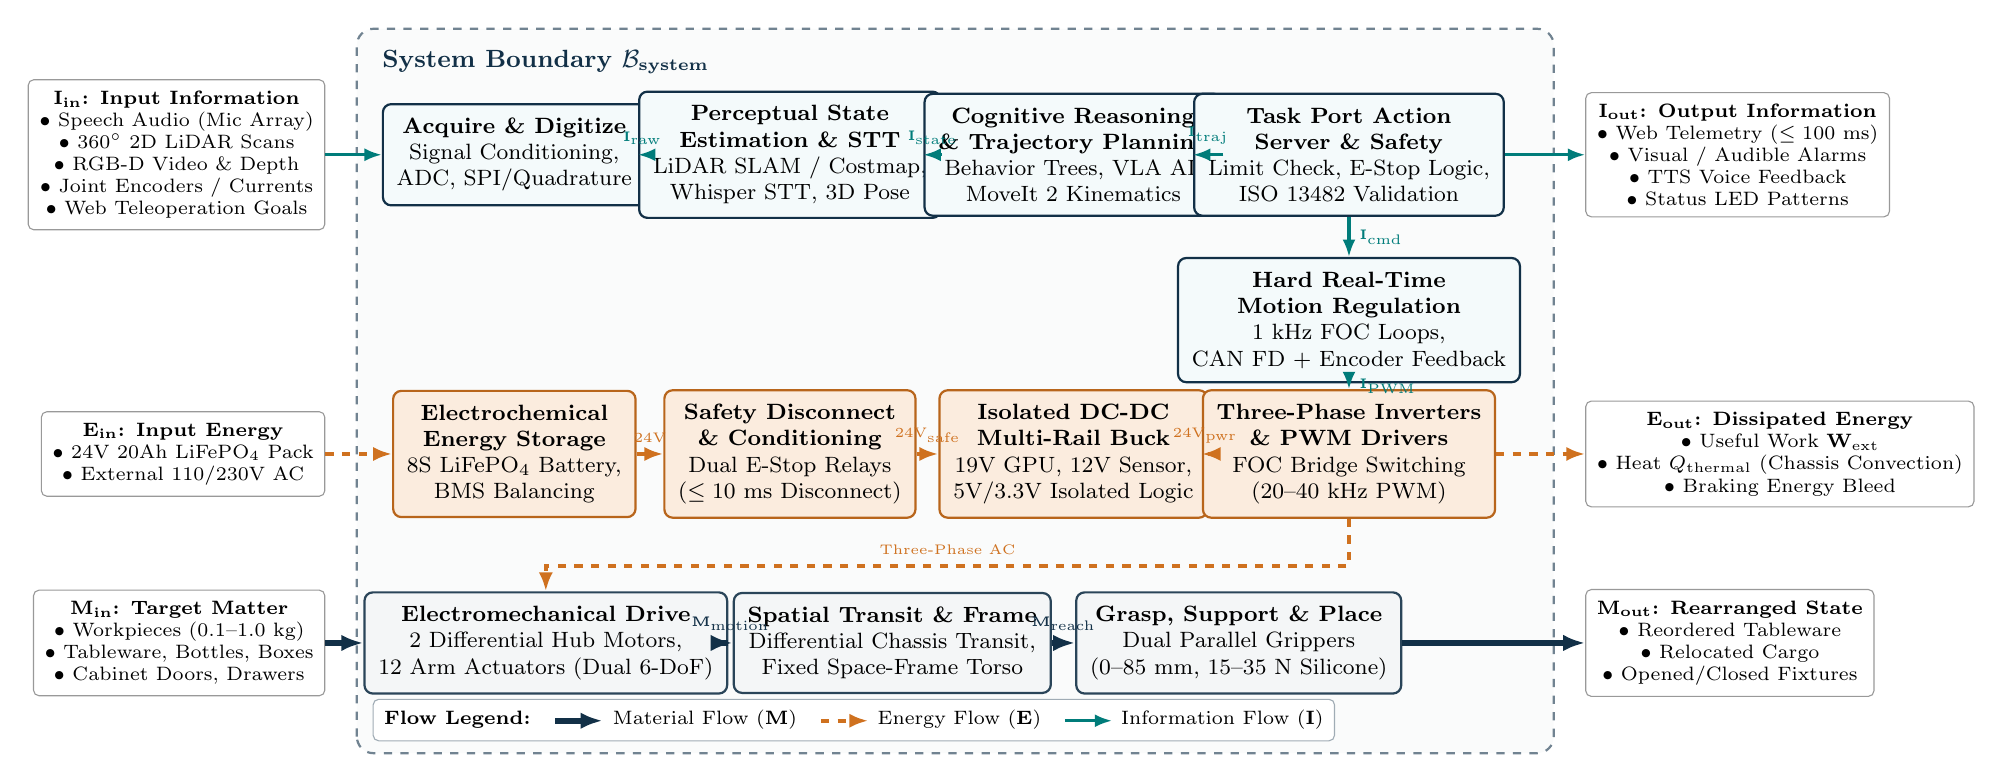
\begin{tikzpicture}[
    >=Latex,
    node distance=0.8cm and 0.9cm,
    font=\footnotesize,
    f_block/.style={draw=navy, fill=sky!30, rounded corners=3pt, thick, align=center, inner sep=5pt, minimum height=1.1cm},
    e_block/.style={draw=orange!80!black, fill=orange!15, rounded corners=3pt, thick, align=center, inner sep=5pt, minimum height=1.1cm},
    m_block/.style={draw=navy!90, fill=pale, rounded corners=3pt, thick, align=center, inner sep=5pt, minimum height=1.1cm},
    io_node/.style={draw=gray!80, fill=white, rounded corners=2pt, align=center, inner sep=4pt, font=\scriptsize},
    flowM/.style={-{Latex[length=2.8mm]}, line width=2.0pt, navy},
    flowE/.style={-{Latex[length=2.4mm]}, line width=1.4pt, orange!90!black, dashed},
    flowI/.style={-{Latex[length=2.2mm]}, line width=1.1pt, teal}
]

  % --- System Boundary Box Coordinates ---
  \draw[navy!60, dashed, thick, rounded corners=6pt, fill=navy!2] (0, -0.6) rectangle (15.2, 8.6);
  \node[anchor=north west, font=\bfseries\small, text=navy] at (0.2, 8.45) {System Boundary $\mathcal{B}_{\text{system}}$};

  % =========================================================================
  % ROW 1: INFORMATION FLOW PIPELINE (y ~ 7.0)
  % =========================================================================
  \node[io_node, anchor=east] (in_I) at (-0.4, 7.0) {\textbf{$\mathbf{I}_{\text{in}}$: Input Information}\\$\bullet$ Speech Audio (Mic Array)\\$\bullet$ $360^\circ$ 2D LiDAR Scans\\$\bullet$ RGB-D Video \& Depth\\$\bullet$ Joint Encoders / Currents\\$\bullet$ Web Teleoperation Goals};

  \node[f_block, minimum width=2.6cm] (f_sense) at (2.0, 7.0) {\textbf{Acquire \& Digitize}\\Signal Conditioning,\\ADC, SPI/Quadrature};

  \node[f_block, minimum width=2.8cm] (f_perceive) at (5.5, 7.0) {\textbf{Perceptual State}\\\textbf{Estimation \& STT}\\LiDAR SLAM / Costmap,\\Whisper STT, 3D Pose};

  \node[f_block, minimum width=2.8cm] (f_plan) at (9.1, 7.0) {\textbf{Cognitive Reasoning}\\\textbf{\& Trajectory Planning}\\Behavior Trees, VLA AI,\\MoveIt 2 Kinematics};

  \node[f_block, minimum width=2.6cm] (f_supervise) at (12.6, 7.0) {\textbf{Task Port Action}\\\textbf{Server \& Safety}\\Limit Check, E-Stop Logic,\\ISO 13482 Validation};

  \node[f_block, minimum width=2.8cm] (f_control) at (12.6, 4.9) {\textbf{Hard Real-Time}\\\textbf{Motion Regulation}\\$1\text{ kHz}$ FOC Loops,\\CAN FD + Encoder Feedback};

  \node[io_node, anchor=west] (out_I) at (15.6, 7.0) {\textbf{$\mathbf{I}_{\text{out}}$: Output Information}\\$\bullet$ Web Telemetry ($\le 100\text{ ms}$)\\$\bullet$ Visual / Audible Alarms\\$\bullet$ TTS Voice Feedback\\$\bullet$ Status LED Patterns};

  % Information connections
  \draw[flowI] (in_I.east) -- (f_sense.west);
  \draw[flowI] (f_sense.east) -- node[above, font=\tiny]{$\mathbf{I}_{\text{raw}}$} (f_perceive.west);
  \draw[flowI] (f_perceive.east) -- node[above, font=\tiny]{$\mathbf{I}_{\text{state}}$} (f_plan.west);
  \draw[flowI] (f_plan.east) -- node[above, font=\tiny]{$\mathbf{I}_{\text{traj}}$} (f_supervise.west);
  \draw[flowI] (f_supervise.south) -- node[right, font=\tiny]{$\mathbf{I}_{\text{cmd}}$} (f_control.north);
  \draw[flowI] (f_supervise.east) -- (out_I.west);

  % =========================================================================
  % ROW 2: ENERGY FLOW PIPELINE (y ~ 3.2)
  % =========================================================================
  \node[io_node, anchor=east] (in_E) at (-0.4, 3.2) {\textbf{$\mathbf{E}_{\text{in}}$: Input Energy}\\$\bullet$ $24\text{V } 20\text{Ah LiFePO}_4$ Pack\\$\bullet$ External $110/230\text{V}$ AC};

  \node[e_block, minimum width=2.6cm] (f_store) at (2.0, 3.2) {\textbf{Electrochemical}\\\textbf{Energy Storage}\\$8\text{S LiFePO}_4$ Battery,\\BMS Balancing};

  \node[e_block, minimum width=2.8cm] (f_estop) at (5.5, 3.2) {\textbf{Safety Disconnect}\\\textbf{\& Conditioning}\\Dual E-Stop Relays\\($\le 10\text{ ms}$ Disconnect)};

  \node[e_block, minimum width=2.8cm] (f_dcdc) at (9.1, 3.2) {\textbf{Isolated DC-DC}\\\textbf{Multi-Rail Buck}\\$19\text{V}$ GPU, $12\text{V}$ Sensor,\\$5\text{V}/3.3\text{V}$ Isolated Logic};

  \node[e_block, minimum width=2.6cm] (f_inverter) at (12.6, 3.2) {\textbf{Three-Phase Inverters}\\\textbf{\& PWM Drivers}\\FOC Bridge Switching\\($20\text{--}40\text{ kHz}$ PWM)};

  % Energy internal connections
  \draw[flowE] (in_E.east) -- (f_store.west);
  \draw[flowE] (f_store.east) -- node[above, font=\tiny]{$24\text{V}$} (f_estop.west);
  \draw[flowE] (f_estop.east) -- node[above, font=\tiny]{$24\text{V}_{\text{safe}}$} (f_dcdc.west);
  \draw[flowE] (f_dcdc.east) -- node[above, font=\tiny]{$24\text{V}_{\text{pwr}}$} (f_inverter.west);

  % Regulated sensor and compute rails are summarized in the DC-DC block.

  % Control signals to inverter
  \draw[flowI] (f_control.south) -- node[right, font=\tiny]{$\mathbf{I}_{\text{PWM}}$} (f_inverter.north);

  % =========================================================================
  % ROW 3: MATERIAL FLOW & ACTUATION PIPELINE (y ~ 0.8)
  % =========================================================================
  \node[io_node, anchor=east] (in_M) at (-0.4, 0.8) {\textbf{$\mathbf{M}_{\text{in}}$: Target Matter}\\$\bullet$ Workpieces ($0.1\text{--}1.0\text{ kg}$)\\$\bullet$ Tableware, Bottles, Boxes\\$\bullet$ Cabinet Doors, Drawers};

  \node[m_block, minimum width=3.4cm] (f_actuate) at (2.4, 0.8) {\textbf{Electromechanical Drive}\\2 Differential Hub Motors,\\12 Arm Actuators (Dual 6-DoF)};

  \node[m_block, minimum width=3.6cm] (f_transport) at (6.8, 0.8) {\textbf{Spatial Transit \& Frame}\\Differential Chassis Transit,\\Fixed Space-Frame Torso};

  \node[m_block, minimum width=3.4cm] (f_grip) at (11.2, 0.8) {\textbf{Grasp, Support \& Place}\\Dual Parallel Grippers\\($0\text{--}85\text{ mm}$, $15\text{--}35\text{ N}$ Silicone)};

  \node[io_node, anchor=west] (out_M) at (15.6, 0.8) {\textbf{$\mathbf{M}_{\text{out}}$: Rearranged State}\\$\bullet$ Reordered Tableware\\$\bullet$ Relocated Cargo\\$\bullet$ Opened/Closed Fixtures};

  % Power conversion to mechanical work
  \draw[flowE] (f_inverter.south) -- ++(0, -0.6) -| node[pos=0.25, above, font=\tiny]{Three-Phase AC} (f_actuate.north);

  % Material flow connections
  \draw[flowM] (in_M.east) -- (f_actuate.west);
  \draw[flowM] (f_actuate.east) -- node[above, font=\tiny]{$\mathbf{M}_{\text{motion}}$} (f_transport.west);
  \draw[flowM] (f_transport.east) -- node[above, font=\tiny]{$\mathbf{M}_{\text{reach}}$} (f_grip.west);
  \draw[flowM] (f_grip.east) -- (out_M.west);

  % Thermal / Mechanical energy dissipation
  \node[io_node, anchor=west] (out_E) at (15.6, 3.2) {\textbf{$\mathbf{E}_{\text{out}}$: Dissipated Energy}\\$\bullet$ Useful Work $\mathbf{W}_{\text{ext}}$\\$\bullet$ Heat $Q_{\text{thermal}}$ (Chassis Convection)\\$\bullet$ Braking Energy Bleed};
  \draw[flowE] (f_inverter.east) -- (out_E.west);

  % Encoder and current feedback return through the CAN fieldbus noted in the control block.

  % =========================================================================
  % LEGEND (y ~ -0.1)
  % =========================================================================
  \node[anchor=south west, font=\scriptsize, draw=navy!40, fill=white, rounded corners=2pt, inner sep=4pt] at (0.2, -0.45) {
    \textbf{Flow Legend:}\quad
    \tikz[baseline=-0.5ex]{\draw[flowM] (0,0) -- (0.6,0);} Material Flow ($\mathbf{M}$)\quad
    \tikz[baseline=-0.5ex]{\draw[flowE] (0,0) -- (0.6,0);} Energy Flow ($\mathbf{E}$)\quad
    \tikz[baseline=-0.5ex]{\draw[flowI] (0,0) -- (0.6,0);} Information Flow ($\mathbf{I}$)
  };

\end{tikzpicture}%
}
\caption{Comprehensive functional structure of the modular semi-humanoid platform in accordance with VDI~2206, showing the interconnected transformation of Material ($\mathbf{M}$), Energy ($\mathbf{E}$), and Information ($\mathbf{I}$) flows across the system boundary.}
\label{fig:functional_structure}
\end{figure}

\section{System Architecture and Multi-Rate Topology}
\label{sec:system_architecture}

\subsection{Architectural Philosophy: Decoupling Cognition from Determinism}
In modern robotic manipulation, integrating high-capacity, probabilistic machine learning models---such as Vision-Language-Action (VLA) policies and Large Language Models (LLMs)---into physical embodied systems presents a fundamental architectural dilemma. Deep learning foundation models offer unprecedented open-world semantic reasoning and general-purpose affordance discovery~\cite{openvla,rtx}; however, their execution latencies are inherently stochastic ($100\text{--}300\text{ ms}$), their outputs are uncertified with respect to safety constraints, and their inferences are subject to out-of-distribution hallucinations. Conversely, the physical plant of a semi-humanoid robot demands deterministic, millisecond-level feedback loops to guarantee kinematic stability, collision avoidance, and non-destructive impedance control~\cite{ros2,moveit2}.

To resolve this dichotomy, the system architecture of the proposed semi-humanoid platform is structured upon a strict separation between \emph{cognitive intent generation}, \emph{deterministic motion planning}, and \emph{hard real-time safety enforcement}. Guided by the VDI~2206 mechatronic systems engineering methodology~\cite{vdi2206}, the platform architecture enforces a strict hierarchical topology wherein non-deterministic AI models act exclusively as advisory goal proposers. Downstream middleware and embedded safety domains act as impenetrable supervisory barriers, validating, projecting, and bounding all motion commands prior to physical actuation.

\subsection{Hierarchical Multi-Rate Execution Topology}
\label{subsec:multi_rate_hierarchy}
The computational and control architecture is organized into four distinct execution tiers operating at discrete update frequencies. Each tier possesses strict timing budgets, designated communication protocols, bounded jitter thresholds, and clearly delineated functional scopes, as summarized in Table~\ref{tab:multi_rate_tiers}.

\begin{table}[ht]
\centering\small
\caption{Hierarchical multi-rate execution topology and timing budgets.}
\label{tab:multi_rate_tiers}
\begin{tabularx}{\textwidth}{@{}p{2.0cm}Xp{2.0cm}p{3.1cm}p{2.9cm}@{}}
\toprule
\textbf{Tier} & \textbf{Functional Scope \& Key Components} & \textbf{Rate / Jitter} & \textbf{Compute Domain} & \textbf{I/O \& Protocol} \\
\midrule
\textbf{Tier 1: Cognition \& HRI} &
Whisper STT, VLA goal proposal (OpenVLA / $\pi_0$), semantic scene grounding, Web Dashboard telemetry streaming. &
$5\text{--}10\text{ Hz}$ \newline ($\pm 50\text{ ms}$) &
NVIDIA Jetson Orin NX (GPU Tensor Cores) &
Shared Memory / Zero-Copy, WebRTC, WebSocket \\
\addlinespace
\textbf{Tier 2: Mission \& Planning} &
BehaviorTree.CPP engine, Nav2 costmaps (MPPI/DWB), MoveIt~2 collision-free Cartesian trajectory generation. &
$30\text{--}50\text{ Hz}$ \newline ($<5\text{ ms}$) &
NVIDIA Jetson Orin NX (PREEMPT\_RT Linux Cores) &
ROS~2 Action Servers \& Topics (Cyclone DDS) \\
\addlinespace
\textbf{Tier 3: Robot Integration} &
\texttt{ros2\_control} manager, UKF state fusion (IMU + odometry), spline interpolation, Cartesian admittance. &
$100\text{--}250\text{ Hz}$ \newline ($<1\text{ ms}$) &
NVIDIA Jetson Orin NX (Pinned Real-Time Core) &
micro-ROS / SocketCAN, USB-to-CAN Gateway \\
\addlinespace
\textbf{Tier 4: Safety \& Actuation} &
Motor FOC current loops, encoder reading, 1~Mbps CAN commutation, hardware E-Stop, thermal/current limit watchdogs. &
$500\text{--}1000\text{ Hz}$ \newline ($<50\ \mu\text{s}$) &
Distributed MCUs (ESP32-WROOM-32 RTOS) &
CAN 2.0B (TWAI), Half-Duplex TTL, Hardwired Loop \\
\bottomrule
\end{tabularx}
\end{table}

\subsubsection{Tier 1: Cognition and Human-Robot Interaction (5--10 Hz)}
Tier~1 executes non-deterministic, compute-intensive artificial intelligence workloads hosted on the 16~GB NVIDIA Jetson Orin NX edge system-on-chip (SoC). This layer processes multimodal sensory observations, including streaming RGB-D images from the Intel RealSense head camera, planar laser scans from the base LiDAR, and far-field audio captured by the ReSpeaker dual-microphone array.
\begin{itemize}[leftmargin=1.5em]
  \item \textbf{Speech and Dialogue Processing:} Far-field acoustic streams are pre-processed using beamforming, acoustic echo cancellation (AEC), and noise suppression before passing to an optimized Whisper-class automatic speech recognition (ASR) engine. The transcribed natural language prompt is parsed into semantic intent tokens.
  \item \textbf{Vision-Language-Action (VLA) Inference:} Open-vocabulary visual grounding models identify target objects and spatial fixtures, while quantized VLA models (e.g., OpenVLA~\cite{openvla} or $\pi_0$) infer high-level end-effector affordance vectors. Because foundation model inference times fluctuate ($100\text{--}200\text{ ms}$), Tier~1 operates strictly asynchronously.
  \item \textbf{Web Dashboard Telemetry:} Compressed video streams (via WebRTC) and state variables are served to external browser clients at $10\text{ Hz}$ via a lightweight WebSocket bridge (\texttt{rosbridge\_suite}).
\end{itemize}
Outputs from Tier~1 take the form of unverified spatial delta proposals $\Delta\mathbf{x}_{\text{AI}}$ or symbolic skill action requests dispatched to the Task Port gateway.

\subsubsection{Tier 2: Mission Orchestration and Motion Planning (30--50 Hz)}
Tier~2 coordinates the robot's autonomy pipeline, reconciling symbolic high-level tasks with geometric and spatial constraints. Running under Ubuntu 22.04 LTS with the PREEMPT\_RT real-time kernel patch on dedicated CPU cores, this tier enforces deterministic synchronization:
\begin{itemize}[leftmargin=1.5em]
  \item \textbf{Behavior Tree Orchestrator:} System mission states are governed by a reactive decision tree implemented in \texttt{BehaviorTree.CPP}~\cite{behaviortrees}. The tree maintains lifecycle states, validates skill preconditions, manages parallel execution of base transit and manipulator posture adjustments, and triggers explicit recovery branches upon anomalous conditions.
  \item \textbf{Mobile Base Navigation (Nav2):} Autonomous base navigation is executed via the Nav2 framework~\cite{nav2}. Planar LiDAR scans and ultrasonic proximity readings populate rolling 2D costmaps. Global paths are computed using Smac 2D grid search, while local path tracking is maintained at $30\text{--}50\text{ Hz}$ using Model Predictive Path Integral (MPPI) or Dynamic Window Approach (DWB) controllers with adaptive deceleration zones.
  \item \textbf{Dual-Arm Manipulation Planning (MoveIt 2):} Kinematic inversions, joint trajectory optimization, and collision avoidance are managed by MoveIt~2~\cite{moveit2}. The planning scene integrates geometric bounding representations of the mobile chassis, torso, and active 3D voxel representations of the environment. Trajectories are parameterized using jerk-limited quintic polynomial splines.
\end{itemize}

\subsubsection{Tier 3: Robot Integration and Middleware (100--250 Hz)}
Tier~3 forms the real-time middleware abstraction layer, establishing a deterministic boundary between high-level ROS~2 nodes and low-level embedded hardware interfaces. Running on an isolated CPU core pinned with highest FIFO scheduling priority (\texttt{SCHED\_FIFO}, priority 90):
\begin{itemize}[leftmargin=1.5em]
  \item \textbf{\texttt{ros2\_control} Hardware Abstraction:} Centralizes joint-space resource claiming and controller lifecycle management. It translates high-level trajectory waypoints into cyclic joint position, velocity, and effort setpoints.
  \item \textbf{Multi-Sensor State Fusion:} An Unscented Kalman Filter (UKF) fuses wheel encoder odometry, torso orientation data from the BNO085 9-DOF IMU, and 2D scan-matching odometry to generate a high-frequency, drift-resistant state estimate ($SE(3)$ base and link poses) at $200\text{ Hz}$.
  \item \textbf{Trajectory Interpolation and Admittance Regulation:} Converts $50\text{ Hz}$ planner waypoints into smooth $200\text{ Hz}$ reference profiles via cubic Hermite splines. In contact-rich manipulation tasks, a Cartesian admittance filter modulates reference trajectories based on motor phase-current feedback:
  \begin{equation}
    \mathbf{M}_d (\ddot{\mathbf{x}}_d - \ddot{\mathbf{x}}_r) + \mathbf{D}_d (\dot{\mathbf{x}}_d - \dot{\mathbf{x}}_r) + \mathbf{K}_d (\mathbf{x}_d - \mathbf{x}_r) = \mathbf{F}_{\text{ext}},
    \label{eq:admittance_filter}
  \end{equation}
  where $\mathbf{M}_d, \mathbf{D}_d, \mathbf{K}_d$ represent the desired virtual inertia, damping, and stiffness matrices, and $\mathbf{F}_{\text{ext}}$ is the estimated contact wrench.
\end{itemize}

\subsubsection{Tier 4: Safety and Embedded Actuation (500--1000 Hz)}
Tier~4 resides entirely within bare-metal and real-time firmware executing on distributed Espressif ESP32-WROOM-32 microcontrollers and the integrated Field-Oriented Control (FOC) drivers of the CubeMars AK70-10 Quasi-Direct Drive (QDD) actuators.
\begin{itemize}[leftmargin=1.5em]
  \item \textbf{Deterministic Fieldbus Execution:} Operates on a synchronous $1\text{ ms}$ cycle ($1000\text{ Hz}$) across a 1~Mbps Controller Area Network (CAN 2.0B / TWAI) and a high-speed half-duplex TTL bus ($1\text{ Mbps}$). The ESP32 coordinators broadcast cyclic torque setpoints and gather 14-bit absolute encoder feedback.
  \item \textbf{Local Commutation and Current Regulation:} The internal FOC drivers of the AK70-10 actuators close current and velocity loops natively at up to $20\text{ kHz}$, clamping motor phase currents to safe thermal envelopes.
  \item \textbf{Hardware Safety Interlocks and Watchdogs:} Dedicated FreeRTOS tasks execute hardware watchdog resets, check fieldbus packet continuity, monitor motor temperatures ($T_{\text{winding}} < 80^\circ\text{C}$), and monitor the hardwired Emergency Stop (E-Stop) loop. Upon bus packet dropout exceeding $10\text{ ms}$ or E-Stop assertion, firmware triggers dynamic regenerative braking and contactor isolation.
\end{itemize}

\subsection{Mathematical Formulation of the Command Contract and Safety Projection}
\label{subsec:command_contract}
To guarantee operational safety without compromising cognitive adaptability, all commands flowing from Tier~1 and Tier~2 into Tier~3 must satisfy a formal \emph{Command Contract}. Let the operational state of the robotic platform at time $t$ be represented by the generalized state vector $\mathbf{x}(t) \in \mathcal{X}$, where:
\begin{equation}
  \mathbf{x}(t) = \begin{bmatrix} \mathbf{p}_{\text{base}} \\ \theta_{\text{base}} \\ \mathbf{q}_{\text{arms}} \\ \mathbf{q}_{\text{grip}} \\ \mathbf{q}_{\text{head}} \end{bmatrix} \in SE(2) \times \mathbb{R}^{12} \times \mathbb{R}^2 \times \mathbb{R}^2,
\end{equation}
and let $\mathbf{q} \in \mathcal{Q} \subset \mathbb{R}^{18}$ denote the complete active degree-of-freedom configuration vector (2 base drive wheels + 12 arm joints + 2 parallel grippers + 2 pan-tilt head joints).

When the cognitive VLA policy or external teleoperator dispatches an unconstrained configuration or Cartesian displacement delta $\Delta\mathbf{x}_{\text{AI}}$, this command cannot be directly committed to the actuator controllers. Instead, the admissible reference setpoint $\mathbf{x}_{\text{ref}}$ is computed via a constrained safety projection operator:
\begin{equation}
  \mathbf{x}_{\text{ref}} = \Pi_{\mathcal{F}(\mathbf{q}, \mathcal{E}, \mathcal{S})}\left(\mathbf{x} + \Delta\mathbf{x}_{\text{AI}}\right),
  \label{eq:safety_projection}
\end{equation}
where $\mathcal{F}(\mathbf{q}, \mathcal{E}, \mathcal{S}) \subset \mathcal{X}$ defines the time-varying, closed and convex set of verified physically feasible and collision-free operational states. The projection operator $\Pi_{\mathcal{F}}$ is mathematically defined as the constrained quadratic optimization:
\begin{equation}
  \Pi_{\mathcal{F}}(\mathbf{y}) = \arg\min_{\mathbf{z} \in \mathcal{F}(\mathbf{q}, \mathcal{E}, \mathcal{S})} \frac{1}{2} \|\mathbf{z} - \mathbf{y}\|_{\mathbf{W}}^2 = \arg\min_{\mathbf{z} \in \mathcal{F}(\mathbf{q}, \mathcal{E}, \mathcal{S})} \frac{1}{2} (\mathbf{z} - \mathbf{y})^T \mathbf{W} (\mathbf{z} - \mathbf{y}),
  \label{eq:projection_optimization}
\end{equation}
where $\mathbf{W} \in \mathbb{R}^{m \times m}$ is a symmetric positive-definite weighting matrix prioritizing structural components (e.g., heavily penalizing base tipping while permitting compliant arm deflections).

\subsubsection{Constrained Feasibility Set Formulation}
The admissible manifold $\mathcal{F}(\mathbf{q}, \mathcal{E}, \mathcal{S})$ is formed by the intersection of four rigorous physical constraint sets:
\begin{equation}
  \mathcal{F}(\mathbf{q}, \mathcal{E}, \mathcal{S}) = \mathcal{C}_{\text{kin}} \cap \mathcal{C}_{\text{stab}} \cap \mathcal{C}_{\text{env}}(\mathcal{E}) \cap \mathcal{C}_{\text{safe}}(\mathcal{S}).
  \label{eq:feasibility_intersection}
\end{equation}

\begin{enumerate}[leftmargin=1.5em]
  \item \textbf{Kinematic and Velocity Bounds ($\mathcal{C}_{\text{kin}}$):}
  Enforces physical joint rotation limits, velocity saturation, and acceleration limits:
  \begin{equation}
    \mathcal{C}_{\text{kin}} = \left\{ \mathbf{x} = \mathbf{f}_{\text{kin}}(\mathbf{q}) \;\middle|\;
    \begin{aligned}
      \mathbf{q}_{\min} \le \mathbf{q} \le \mathbf{q}_{\max}, \\
      -\dot{\mathbf{q}}_{\max} \le \mathbf{J}^{\dagger}(\mathbf{q}) \dot{\mathbf{x}} \le \dot{\mathbf{q}}_{\max}, \\
      -\ddot{\mathbf{q}}_{\max} \le \ddot{\mathbf{q}} \le \ddot{\mathbf{q}}_{\max}
    \end{aligned}
    \right\},
  \end{equation}
  where $\mathbf{f}_{\text{kin}}(\cdot)$ denotes the forward kinematics mapping, $\mathbf{J}(\mathbf{q})$ is the geometric manipulator Jacobian, and $\mathbf{J}^{\dagger}$ is its Moore-Penrose pseudoinverse.

  \item \textbf{Dynamic Base Stability and Center of Mass Envelope ($\mathcal{C}_{\text{stab}}$):}
  To prevent chassis rollover during high-acceleration torso pitching or fast manipulator reaching with heavy payloads, the dynamic Zero-Moment Point (ZMP) $\mathbf{p}_{\text{ZMP}}$ must reside strictly within a contracted interior of the chassis support polygon $\mathcal{P}_{\text{support}}$ formed by the two 200~mm drive wheels and dual 100~mm casters:
  \begin{equation}
    \mathcal{C}_{\text{stab}} = \left\{ \mathbf{x} \;\middle|\; \mathbf{p}_{\text{ZMP}}(\mathbf{q}, \ddot{\mathbf{q}}, \mathbf{a}_{\text{base}}) \in \operatorname{int}_{\delta}\left(\mathcal{P}_{\text{support}}\right) \right\},
  \end{equation}
  where the planar ZMP is evaluated dynamically from the lumped mass distribution:
  \begin{equation}
    \mathbf{p}_{\text{ZMP}} = \frac{\sum_{i=1}^{N} m_i \left(\ddot{z}_i + g\right) \mathbf{r}_{i,xy} - \sum_{i=1}^{N} m_i \ddot{\mathbf{r}}_{i,xy} z_i}{\sum_{i=1}^{N} m_i \left(\ddot{z}_i + g\right)},
  \end{equation}
  with $m_i$ and $\mathbf{r}_i = [\mathbf{r}_{i,xy}^T, z_i]^T$ representing the mass and Cartesian position of link $i$, $g = 9.81\text{ m/s}^2$ the gravitational acceleration, and $\operatorname{int}_{\delta}(\cdot)$ denoting a conservative safety margin contraction of $\delta = 35\text{ mm}$ from the physical polygon boundary.

  \item \textbf{Environmental Obstacle Clearance ($\mathcal{C}_{\text{env}}(\mathcal{E})$):}
  Based on real-time 3D Signed Distance Fields (SDF) and 2D Nav2 local costmaps generated from the environment perception state $\mathcal{E}$, every rigid body link $\mathcal{B}_k(\mathbf{q})$ must maintain a positive distance margin from external obstacles $\mathcal{O}_{\text{env}}$:
  \begin{equation}
    \mathcal{C}_{\text{env}}(\mathcal{E}) = \left\{ \mathbf{x} \;\middle|\; \min_{k} \operatorname{dist}\left(\mathcal{B}_k(\mathbf{q}), \mathcal{O}_{\text{env}}\right) \ge d_{\text{safe}} \right\},
  \end{equation}
  where $d_{\text{safe}} = 0.05\text{ m}$ for static workspace fixtures and $d_{\text{safe}} = 0.25\text{ m}$ for dynamic human obstacles.

  \item \textbf{Supervisory Safety State ($\mathcal{C}_{\text{safe}}(\mathcal{S})$):}
  Governed by discrete safety system variables $\mathcal{S}$:
  \begin{equation}
    \mathcal{C}_{\text{safe}}(\mathcal{S}) = \left\{ \mathbf{x} \;\middle|\;
    \begin{aligned}
      &E_{\text{stop}} = \text{NORMAL}, \quad \text{SoC} \ge 10\%, \\
      &T_{\text{actuator}} \le 80^\circ\text{C}, \quad \|\mathbf{F}_{\text{contact}}\| \le F_{\text{threshold}}
    \end{aligned}
    \right\}.
  \end{equation}
\end{enumerate}

\subsubsection{Anomaly Recovery and Observable Veto Semantics}
Crucially, when the projection operator $\Pi_{\mathcal{F}}$ clamps an AI proposal, or when numerical infeasibility occurs, the command is \emph{not} discarded silently. Let the projection residual be:
\begin{equation}
  \varepsilon_{\text{proj}} = \left\| \Pi_{\mathcal{F}(\mathbf{q}, \mathcal{E}, \mathcal{S})}\left(\mathbf{x} + \Delta\mathbf{x}_{\text{AI}}\right) - \left(\mathbf{x} + \Delta\mathbf{x}_{\text{AI}}\right) \right\|.
\end{equation}
If $\varepsilon_{\text{proj}} > \varepsilon_{\text{tol}}$ (where $\varepsilon_{\text{tol}} = 0.04\text{ m}$ in task space), Tier~3 immediately raises an observable \texttt{\small SafetyProjectionVeto} event over the ROS~2 middleware. This event halts downstream setpoint transmission, activates a smooth joint-space deceleration profile, and passes an execution failure signal to the Tier~2 \texttt{BehaviorTree.CPP} coordinator. The behavior tree responds by executing structured recovery nodes (e.g., retrying with an alternative grasp pose, repositioning the mobile base, or prompting the user via the Web Dashboard).

\subsection{System-Level Mechatronic Interconnection Architecture}
\label{subsec:mechatronic_interconnection}
To guarantee electrical isolation, deterministic communication, and absolute human safety, the semi-humanoid platform is partitioned into four physically distinct interconnection networks:
\begin{enumerate}[leftmargin=1.5em]
  \item \textbf{Power Distribution Network:} Galvanically isolates high-noise inductive actuator loads from sensitive digital compute. A central 24V 20Ah LiFePO$_4$ battery pack feeds two branches:
  \begin{itemize}
    \item \emph{Protected Logic Rail (Uncuttable 24V):} Routed directly from the BMS through slow-blow fuses to high-efficiency synchronous DC-DC buck converters supplying regulated $19\text{V}$ (Jetson Orin NX), $12\text{V}$ (head servos and cooling fans), and $5\text{V}$ (ESP32 controllers, sensors, and logic).
    \item \emph{Switched Motor Power Rail (Cuttable 24V):} Routed through a heavy-duty 24V 40A continuous safety contactor relay. This rail supplies the 9$\times$ CubeMars AK70-10 QDD actuators and the dual base BLDC drive motors.
  \end{itemize}
  \item \textbf{Deterministic Fieldbus Network (CAN 2.0B / TWAI at 1 Mbps):} A shared, high-speed differential bus interconnecting the Jetson compute host (via an isolated USB-to-CAN gateway) with the distributed ESP32 microcontrollers and the 9$\times$ AK70-10 QDD internal drivers. Employs 120\,$\Omega$ terminating resistors and shielded twisted-pair (STP) cabling.
  \item \textbf{High-Bandwidth Perception and Telemetry Network:} High-speed point-to-point buses comprising Gigabit Ethernet (1000BASE-T) and USB~3.0/2.0 lines. Interconnects the Intel RealSense RGB-D camera, Slamtec RPLiDAR A1M8, ReSpeaker microphone array, Torso physical panel ports, and dual-band Wi-Fi~6 router.
  \item \textbf{Hardwired Fail-Safe E-Stop Network:} An active-low, dual-channel physical loop connecting mechanical latching mushroom push-buttons (chassis-mounted and optional wireless tether) directly to the coil driver of the 40A safety contactor. Depressing an E-Stop button breaks coil power within $\le 10\text{ ms}$, physically cutting power to all high-torque actuators while maintaining complete power to compute, sensors, telemetry, and error logging.
\end{enumerate}

Figure~\ref{fig:mechatronic_block_diagram} depicts the system-level mechatronic block diagram, detailing the routing of all four independent physical networks across the platform subsystems.

\begin{figure}[htbp]
\centering
\resizebox{\linewidth}{!}{%
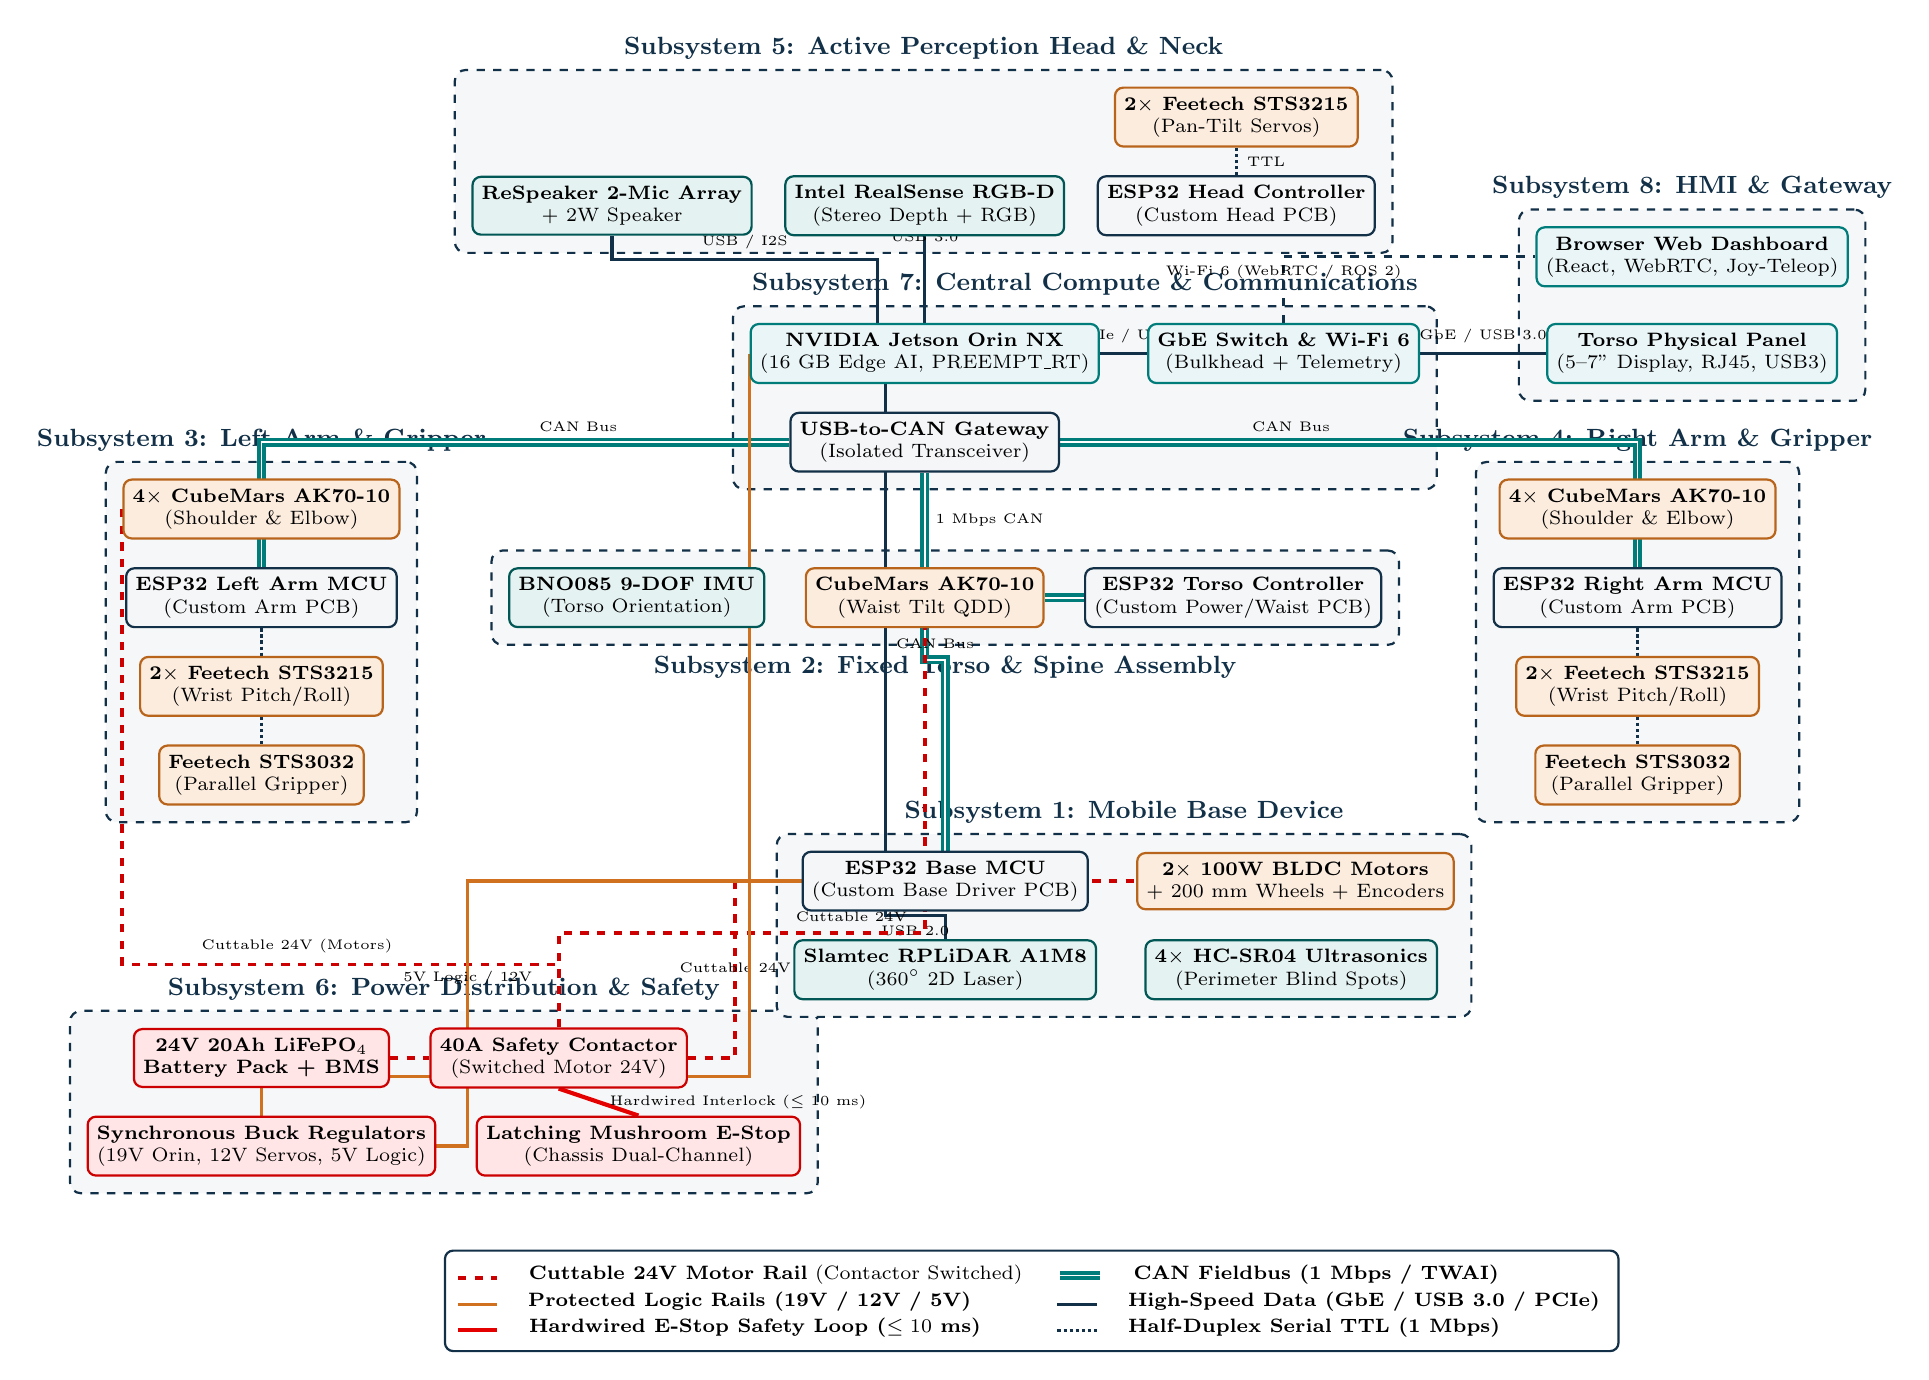
\begin{tikzpicture}[
    node distance=0.55cm and 0.65cm,
    >=Latex,
    every node/.style={font=\scriptsize, align=center},
    subsys_box/.style={draw=navy, fill=navy!4, rounded corners=4pt, dashed, thick, inner sep=6pt},
    comp_compute/.style={draw=teal, fill=sky!60, rounded corners=3pt, thick, minimum width=2.4cm, minimum height=0.75cm},
    comp_mcu/.style={draw=navy, fill=pale, rounded corners=3pt, thick, minimum width=2.2cm, minimum height=0.65cm},
    comp_actuator/.style={draw=orange!80!black, fill=orange!15, rounded corners=3pt, thick, minimum width=2.2cm, minimum height=0.65cm},
    comp_sensor/.style={draw=teal!70!black, fill=teal!10, rounded corners=3pt, thick, minimum width=2.2cm, minimum height=0.65cm},
    comp_power/.style={draw=red!80!black, fill=red!10, rounded corners=3pt, thick, minimum width=2.2cm, minimum height=0.65cm},
    net_pwr_cut/.style={draw=red!80!black, line width=1.4pt, dashed},
    net_pwr_log/.style={draw=orange!90!black, line width=1.2pt},
    net_can/.style={draw=teal, line width=1.3pt, double},
    net_data/.style={draw=navy, line width=1.2pt},
    net_estop/.style={draw=red!90!black, line width=1.5pt}
]

  % Subsystem 7: Central Compute
  \node[comp_compute] (jetson) {\textbf{NVIDIA Jetson Orin NX}\\(16 GB Edge AI, PREEMPT\_RT)};
  \node[comp_compute, right=0.6cm of jetson] (switch) {\textbf{GbE Switch \& Wi-Fi 6}\\(Bulkhead + Telemetry)};
  \node[comp_mcu, below=0.35cm of jetson] (can_gw) {\textbf{USB-to-CAN Gateway}\\(Isolated Transceiver)};
  \begin{scope}[on background layer]
    \node[subsys_box, fit=(jetson) (switch) (can_gw), label={[navy, font=\bfseries\small]above:Subsystem 7: Central Compute \& Communications}] (box_s7) {};
  \end{scope}

  % Subsystem 5: Perception Head (Above Compute)
  \node[comp_sensor, above=1.1cm of jetson] (cam_head) {\textbf{Intel RealSense RGB-D}\\(Stereo Depth + RGB)};
  \node[comp_sensor, left=0.4cm of cam_head] (mic_head) {\textbf{ReSpeaker 2-Mic Array}\\+ 2W Speaker};
  \node[comp_mcu, right=0.4cm of cam_head] (mcu_head) {\textbf{ESP32 Head Controller}\\(Custom Head PCB)};
  \node[comp_actuator, above=0.35cm of mcu_head] (servo_head) {\textbf{2$\times$ Feetech STS3215}\\(Pan-Tilt Servos)};
  \begin{scope}[on background layer]
    \node[subsys_box, fit=(cam_head) (mic_head) (mcu_head) (servo_head), label={[navy, font=\bfseries\small]above:Subsystem 5: Active Perception Head \& Neck}] (box_s5) {};
  \end{scope}

  % Subsystem 8: HMI & Dashboard (Right of Compute)
  \node[comp_compute, right=1.6cm of switch] (panel_hmi) {\textbf{Torso Physical Panel}\\(5--7'' Display, RJ45, USB3)};
  \node[comp_compute, above=0.45cm of panel_hmi] (web_hmi) {\textbf{Browser Web Dashboard}\\(React, WebRTC, Joy-Teleop)};
  \begin{scope}[on background layer]
    \node[subsys_box, fit=(panel_hmi) (web_hmi), label={[navy, font=\bfseries\small]above:Subsystem 8: HMI \& Gateway}] (box_s8) {};
  \end{scope}

  % Subsystem 2: Torso (Below Compute)
  \node[comp_actuator, below=1.2cm of can_gw] (ak_waist) {\textbf{CubeMars AK70-10}\\(Waist Tilt QDD)};
  \node[comp_sensor, left=0.5cm of ak_waist] (imu_torso) {\textbf{BNO085 9-DOF IMU}\\(Torso Orientation)};
  \node[comp_mcu, right=0.5cm of ak_waist] (mcu_torso) {\textbf{ESP32 Torso Controller}\\(Custom Power/Waist PCB)};
  \begin{scope}[on background layer]
    \node[subsys_box, fit=(ak_waist) (imu_torso) (mcu_torso), label={[navy, font=\bfseries\small]below:Subsystem 2: Fixed Torso \& Spine Assembly}] (box_s2) {};
  \end{scope}

  % Subsystem 3: Left Arm (Left of Torso)
  \node[comp_mcu, left=1.4cm of imu_torso] (mcu_arm_l) {\textbf{ESP32 Left Arm MCU}\\(Custom Arm PCB)};
  \node[comp_actuator, above=0.35cm of mcu_arm_l] (qdd_arm_l) {\textbf{4$\times$ CubeMars AK70-10}\\(Shoulder \& Elbow)};
  \node[comp_actuator, below=0.35cm of mcu_arm_l] (wrist_arm_l) {\textbf{2$\times$ Feetech STS3215}\\(Wrist Pitch/Roll)};
  \node[comp_actuator, below=0.35cm of wrist_arm_l] (grip_l) {\textbf{Feetech STS3032}\\(Parallel Gripper)};
  \begin{scope}[on background layer]
    \node[subsys_box, fit=(mcu_arm_l) (qdd_arm_l) (wrist_arm_l) (grip_l), label={[navy, font=\bfseries\small]above:Subsystem 3: Left Arm \& Gripper}] (box_s3) {};
  \end{scope}

  % Subsystem 4: Right Arm (Right of Torso)
  \node[comp_mcu, right=1.4cm of mcu_torso] (mcu_arm_r) {\textbf{ESP32 Right Arm MCU}\\(Custom Arm PCB)};
  \node[comp_actuator, above=0.35cm of mcu_arm_r] (qdd_arm_r) {\textbf{4$\times$ CubeMars AK70-10}\\(Shoulder \& Elbow)};
  \node[comp_actuator, below=0.35cm of mcu_arm_r] (wrist_arm_r) {\textbf{2$\times$ Feetech STS3215}\\(Wrist Pitch/Roll)};
  \node[comp_actuator, below=0.35cm of wrist_arm_r] (grip_r) {\textbf{Feetech STS3032}\\(Parallel Gripper)};
  \begin{scope}[on background layer]
    \node[subsys_box, fit=(mcu_arm_r) (qdd_arm_r) (wrist_arm_r) (grip_r), label={[navy, font=\bfseries\small]above:Subsystem 4: Right Arm \& Gripper}] (box_s4) {};
  \end{scope}

  % Subsystem 6: Power Distribution & Safety Subsystem (Far Left Bottom)
  \node[comp_power, below=2.6cm of box_s3] (batt) {\textbf{24V 20Ah LiFePO$_4$}\\\textbf{Battery Pack + BMS}};
  \node[comp_power, right=0.5cm of batt] (contactor) {\textbf{40A Safety Contactor}\\(Switched Motor 24V)};
  \node[comp_power, below=0.35cm of batt] (dcdc) {\textbf{Synchronous Buck Regulators}\\(19V Orin, 12V Servos, 5V Logic)};
  \node[comp_power, right=0.5cm of dcdc] (estop_btn) {\textbf{Latching Mushroom E-Stop}\\(Chassis Dual-Channel)};
  \begin{scope}[on background layer]
    \node[subsys_box, fit=(batt) (contactor) (dcdc) (estop_btn), label={[navy, font=\bfseries\small]above:Subsystem 6: Power Distribution \& Safety}] (box_s6) {};
  \end{scope}

  % Subsystem 1: Mobile Base Device (Right Bottom)
  \node[comp_mcu, below=2.6cm of box_s2] (mcu_base) {\textbf{ESP32 Base MCU}\\(Custom Base Driver PCB)};
  \node[comp_actuator, right=0.6cm of mcu_base] (motors_base) {\textbf{2$\times$ 100W BLDC Motors}\\+ 200 mm Wheels + Encoders};
  \node[comp_sensor, below=0.35cm of mcu_base] (lidar_base) {\textbf{Slamtec RPLiDAR A1M8}\\(360$^\circ$ 2D Laser)};
  \node[comp_sensor, right=0.6cm of lidar_base] (sonic_base) {\textbf{4$\times$ HC-SR04 Ultrasonics}\\(Perimeter Blind Spots)};
  \begin{scope}[on background layer]
    \node[subsys_box, fit=(mcu_base) (motors_base) (lidar_base) (sonic_base), label={[navy, font=\bfseries\small]above:Subsystem 1: Mobile Base Device}] (box_s1) {};
  \end{scope}

  % --- INTERCONNECTION LINES ---
  % Route buses behind component cards so wiring cannot obscure labels.
  \begin{scope}[on background layer]
  % High-speed data (Navy solid)
  \draw[net_data] (cam_head.south) -- ++(0,-0.2) -| node[pos=0.25, above, font=\tiny]{USB 3.0} (jetson.north);
  \draw[net_data] (mic_head.south) -- ++(0,-0.3) -| node[pos=0.25, above, font=\tiny]{USB / I2S} ($(jetson.north)+(-0.6,0)$);
  \draw[net_data] (lidar_base.north) -- ++(0,0.3) -| node[pos=0.25, below, font=\tiny]{USB 2.0} ($(jetson.south)+(-0.5,0)$);
  \draw[net_data] (jetson.east) -- node[above, font=\tiny]{PCIe / USB} (switch.west);
  \draw[net_data] (switch.east) -- node[above, font=\tiny]{GbE / USB 3.0} (panel_hmi.west);
  \draw[net_data, dashed] (switch.north) |- node[pos=0.25, above, font=\tiny]{Wi-Fi 6 (WebRTC / ROS 2)} (web_hmi.west);

  % CAN Fieldbus (Teal double line)
  \draw[net_can] (can_gw.south) -- node[right, font=\tiny]{1 Mbps CAN} (ak_waist.north);
  \draw[net_can] (ak_waist.east) -- (mcu_torso.west);
  \draw[net_can] (can_gw.west) -| node[pos=0.2, above, font=\tiny]{CAN Bus} (mcu_arm_l.north);
  \draw[net_can] (can_gw.east) -| node[pos=0.2, above, font=\tiny]{CAN Bus} (mcu_arm_r.north);
  \draw[net_can] (mcu_arm_l.north) -- (qdd_arm_l.south);
  \draw[net_can] (mcu_arm_r.north) -- (qdd_arm_r.south);
  \draw[net_can] (ak_waist.south) -- ++(0,-0.4) -| node[pos=0.25, above, font=\tiny]{CAN Bus} (mcu_base.north);

  % Half-duplex TTL serial chains (navy dashed)
  \draw[net_data, densely dotted] (mcu_head.north) -- node[right, font=\tiny]{TTL} (servo_head.south);
  \draw[net_data, densely dotted] (mcu_arm_l.south) -- (wrist_arm_l.north);
  \draw[net_data, densely dotted] (wrist_arm_l.south) -- (grip_l.north);
  \draw[net_data, densely dotted] (mcu_arm_r.south) -- (wrist_arm_r.north);
  \draw[net_data, densely dotted] (wrist_arm_r.south) -- (grip_r.north);

  % Power: Cuttable 24V (Red dashed)
  \draw[net_pwr_cut] (batt.east) -- (contactor.west);
  \draw[net_pwr_cut] (contactor.north) -- ++(0,0.8) -| node[pos=0.3, above, font=\tiny]{Cuttable 24V (Motors)} (qdd_arm_l.west);
  \draw[net_pwr_cut] (contactor.north) -- ++(0,1.2) -| node[pos=0.4, above, font=\tiny]{Cuttable 24V} (ak_waist.south);
  \draw[net_pwr_cut] (contactor.east) -- ++(0.6,0) |- node[pos=0.3, below, font=\tiny]{Cuttable 24V} (motors_base.west);

  % Power: Protected Logic (Orange solid)
  \draw[net_pwr_log] (batt.south) -- (dcdc.north);
  \draw[net_pwr_log] (dcdc.east) -- ++(0.4,0) |- node[pos=0.35, below, font=\tiny]{5V Logic / 12V} (mcu_base.west);
  \draw[net_pwr_log] (dcdc.north) -- ++(0,0.5) -| node[pos=0.25, above, font=\tiny]{19V / 5V} (jetson.west);

  % E-Stop hardwired loop (Red solid thick)
  \draw[net_estop] (estop_btn.north) -- node[right, font=\tiny]{Hardwired Interlock ($\le 10$ ms)} (contactor.south);

  \end{scope}

  % --- LEGEND ---
  \node[draw=navy, fill=white, rounded corners=3pt, thick, below=0.7cm of box_s6, anchor=north west, inner sep=4pt] (legend) {
    \begin{tabular}{@{}ll@{}}
      \tikz\draw[net_pwr_cut] (0,0) -- (0.5,0); \quad \textbf{Cuttable 24V Motor Rail} (Contactor Switched) &
      \tikz\draw[net_can] (0,0) -- (0.5,0); \quad \textbf{CAN Fieldbus (1 Mbps / TWAI)} \\
      \tikz\draw[net_pwr_log] (0,0) -- (0.5,0); \quad \textbf{Protected Logic Rails (19V / 12V / 5V)} &
      \tikz\draw[net_data] (0,0) -- (0.5,0); \quad \textbf{High-Speed Data (GbE / USB 3.0 / PCIe)} \\
      \tikz\draw[net_estop] (0,0) -- (0.5,0); \quad \textbf{Hardwired E-Stop Safety Loop ($\le 10\text{ ms}$)} &
      \tikz\draw[net_data, densely dotted] (0,0) -- (0.5,0); \quad \textbf{Half-Duplex Serial TTL (1 Mbps)} \\
    \end{tabular}
  };
\end{tikzpicture}%
}
\caption{System-level mechatronic block diagram illustrating the four physically distinct interconnection networks: Switched Motor Power Rail, Protected Logic Power Rails, Deterministic CAN Fieldbus (1~Mbps), High-Speed Perception/Telemetry (GbE/USB~3.0), and the Hardwired Fail-Safe E-Stop Loop.}
\label{fig:mechatronic_block_diagram}
\end{figure}

\section{Detailed Subsystems Mechatronic Design}
\label{sec:subsystems_detail}

\subsection{Modular Device-Level Mechatronic Philosophy}
In accordance with the VDI~2206 guidelines for cyber-physical mechatronic systems~\cite{vdi2206}, the semi-humanoid robotic platform is partitioned into discrete, independently verifiable, and functionally encapsulated \emph{devices}. Rather than treating the robot as a monolithic electro-mechanical assembly, each device integrates its own structural framework, specialized actuators, primary sensing transducers, localized embedded microcontroller (Espressif ESP32-WROOM-32) or central compute module, and standardized communication interfaces.

This modular device abstraction delivers three decisive engineering advantages:
\begin{enumerate}[leftmargin=1.5em]
  \item \textbf{Isolated Unit Testing and Hardware-in-the-Loop (HIL) Verification:} Every subsystem can be powered, calibrated, dynamically tuned, and benchmarked on a standalone test bench before final physical integration onto the chassis.
  \item \textbf{Standardized Bus Architecture and Hot-Swappability:} Devices communicate across standardized physical links (1~Mbps CAN 2.0B / TWAI, half-duplex serial TTL, Gigabit Ethernet, and USB~3.0). Failed assemblies can be replaced rapidly without rewiring the central harness.
  \item \textbf{Decoupled Software and Firmware Maintenance:} Microcontroller firmware manages low-level PID/FOC regulation natively, exposing standardized ROS~2 topics and action endpoints to Tier~2 and Tier~3 software.
\end{enumerate}

Figure~\ref{fig:modular_device_decomposition} illustrates the structural partitioning and logical boundaries across all eight core subsystems of the platform.

\begin{figure}[htbp]
\centering
\resizebox{\linewidth}{!}{%
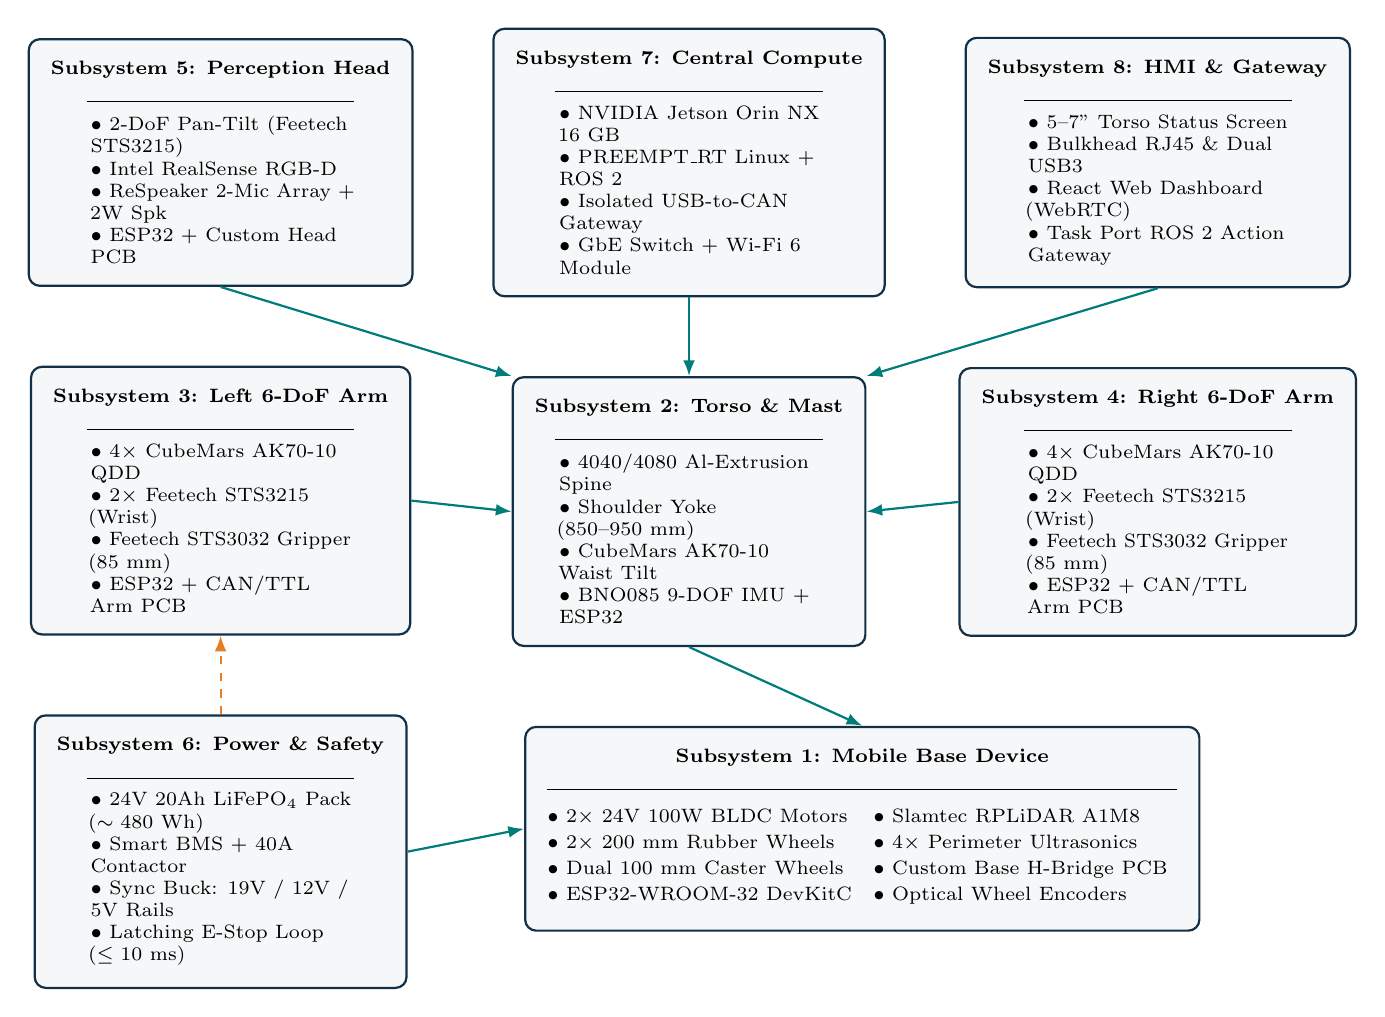
\begin{tikzpicture}[
    node distance=0.6cm and 0.8cm,
    >=Latex,
    every node/.style={font=\scriptsize, align=center},
    subsys_card/.style={draw=navy, fill=navy!4, rounded corners=4pt, thick, inner sep=8pt, minimum width=3.6cm},
    header_style/.style={draw=teal, fill=sky!80, rounded corners=2pt, font=\bfseries\footnotesize, text=navy, minimum width=3.4cm, minimum height=0.55cm},
    item_style/.style={align=left, font=\scriptsize, text width=3.3cm},
    link_arrow/.style={-{Latex[length=2mm]}, thick, teal}
]

  % Row 1: Perception Head & Compute
  \node[subsys_card] (card_s5) {
    \textbf{Subsystem 5: Perception Head}\\[2pt]
    \rule{3.4cm}{0.4pt}\\[4pt]
    \begin{minipage}{3.3cm}\raggedright
      $\bullet$ 2-DoF Pan-Tilt (Feetech STS3215)\\
      $\bullet$ Intel RealSense RGB-D\\
      $\bullet$ ReSpeaker 2-Mic Array + 2W Spk\\
      $\bullet$ ESP32 + Custom Head PCB
    \end{minipage}
  };

  \node[subsys_card, right=1.0cm of card_s5] (card_s7) {
    \textbf{Subsystem 7: Central Compute}\\[2pt]
    \rule{3.4cm}{0.4pt}\\[4pt]
    \begin{minipage}{3.3cm}\raggedright
      $\bullet$ NVIDIA Jetson Orin NX 16 GB\\
      $\bullet$ PREEMPT\_RT Linux + ROS 2\\
      $\bullet$ Isolated USB-to-CAN Gateway\\
      $\bullet$ GbE Switch + Wi-Fi 6 Module
    \end{minipage}
  };

  \node[subsys_card, right=1.0cm of card_s7] (card_s8) {
    \textbf{Subsystem 8: HMI \& Gateway}\\[2pt]
    \rule{3.4cm}{0.4pt}\\[4pt]
    \begin{minipage}{3.3cm}\raggedright
      $\bullet$ 5--7'' Torso Status Screen\\
      $\bullet$ Bulkhead RJ45 \& Dual USB3\\
      $\bullet$ React Web Dashboard (WebRTC)\\
      $\bullet$ Task Port ROS 2 Action Gateway
    \end{minipage}
  };

  % Row 2: Left Arm, Torso, Right Arm
  \node[subsys_card, below=1.0cm of card_s5] (card_s3) {
    \textbf{Subsystem 3: Left 6-DoF Arm}\\[2pt]
    \rule{3.4cm}{0.4pt}\\[4pt]
    \begin{minipage}{3.3cm}\raggedright
      $\bullet$ 4$\times$ CubeMars AK70-10 QDD\\
      $\bullet$ 2$\times$ Feetech STS3215 (Wrist)\\
      $\bullet$ Feetech STS3032 Gripper ($85\text{ mm}$)\\
      $\bullet$ ESP32 + CAN/TTL Arm PCB
    \end{minipage}
  };

  \node[subsys_card, below=1.0cm of card_s7] (card_s2) {
    \textbf{Subsystem 2: Torso \& Mast}\\[2pt]
    \rule{3.4cm}{0.4pt}\\[4pt]
    \begin{minipage}{3.3cm}\raggedright
      $\bullet$ 4040/4080 Al-Extrusion Spine\\
      $\bullet$ Shoulder Yoke ($850\text{--}950\text{ mm}$)\\
      $\bullet$ CubeMars AK70-10 Waist Tilt\\
      $\bullet$ BNO085 9-DOF IMU + ESP32
    \end{minipage}
  };

  \node[subsys_card, below=1.0cm of card_s8] (card_s4) {
    \textbf{Subsystem 4: Right 6-DoF Arm}\\[2pt]
    \rule{3.4cm}{0.4pt}\\[4pt]
    \begin{minipage}{3.3cm}\raggedright
      $\bullet$ 4$\times$ CubeMars AK70-10 QDD\\
      $\bullet$ 2$\times$ Feetech STS3215 (Wrist)\\
      $\bullet$ Feetech STS3032 Gripper ($85\text{ mm}$)\\
      $\bullet$ ESP32 + CAN/TTL Arm PCB
    \end{minipage}
  };

  % Row 3: Power Subsystem & Mobile Base
  \node[subsys_card, below=1.0cm of card_s3] (card_s6) {
    \textbf{Subsystem 6: Power \& Safety}\\[2pt]
    \rule{3.4cm}{0.4pt}\\[4pt]
    \begin{minipage}{3.3cm}\raggedright
      $\bullet$ 24V 20Ah LiFePO$_4$ Pack ($\sim 480\text{ Wh}$)\\
      $\bullet$ Smart BMS + 40A Contactor\\
      $\bullet$ Sync Buck: 19V / 12V / 5V Rails\\
      $\bullet$ Latching E-Stop Loop ($\le 10\text{ ms}$)
    \end{minipage}
  };

  \node[subsys_card, below=1.0cm of card_s2, xshift=2.2cm, minimum width=8.2cm] (card_s1) {
    \textbf{Subsystem 1: Mobile Base Device}\\[2pt]
    \rule{8.0cm}{0.4pt}\\[4pt]
    \begin{minipage}{8.0cm}\raggedright
      \begin{tabular}{@{}p{4.0cm}@{\hspace{4pt}}p{3.8cm}@{}}
        $\bullet$ 2$\times$ 24V 100W BLDC Motors & $\bullet$ Slamtec RPLiDAR A1M8 \\
        $\bullet$ 2$\times$ 200 mm Rubber Wheels & $\bullet$ 4$\times$ Perimeter Ultrasonics \\
        $\bullet$ Dual 100 mm Caster Wheels & $\bullet$ Custom Base H-Bridge PCB \\
        $\bullet$ ESP32-WROOM-32 DevKitC & $\bullet$ Optical Wheel Encoders \\
      \end{tabular}
    \end{minipage}
  };

  % Connecting arrows representing structural and logical coupling
  \draw[link_arrow] (card_s5.south) -- (card_s2.north west);
  \draw[link_arrow] (card_s7.south) -- (card_s2.north);
  \draw[link_arrow] (card_s8.south) -- (card_s2.north east);
  \draw[link_arrow] (card_s3.east) -- (card_s2.west);
  \draw[link_arrow] (card_s4.west) -- (card_s2.east);
  \draw[link_arrow] (card_s2.south) -- (card_s1.north);
  \draw[link_arrow] (card_s6.east) -- (card_s1.west);
  \draw[link_arrow, dashed, orange] (card_s6.north) -- (card_s3.south);

\end{tikzpicture}%
}
\caption{Device-level modular decomposition illustrating the encapsulation of mechanical structures, actuators, embedded electronics, and communications across all eight platform subsystems.}
\label{fig:modular_device_decomposition}
\end{figure}

\subsection{Subsystem 1: Mobile Base Device}
\label{subsec:subsystem_1_base}
The Mobile Base Device provides agile, high-traction, and stable indoor transit across unstructured domestic and industrial floor environments. Rather than utilizing complex, maintenance-intensive Mecanum wheels that suffer from severe slippage, vibration, and debris jamming on standard indoor carpeting, the platform employs a high-traction differential drive kinematic topology paired with dual passive support points.

\subsubsection{Kinematics and Wheel Sizing Rationale}
The drivetrain utilizes two active drive wheels ($D_{\text{wheel}} = 200\text{ mm}$, $b_{\text{wheel}} = 50\text{ mm}$) featuring high-grip vulcanized rubber treads, mounted coaxially with a track gauge of $L = 460\text{ mm}$. The large $200\text{ mm}$ wheel diameter was specifically selected to ensure seamless traversal over standard architectural thresholds ($15\text{--}20\text{ mm}$ height), thick carpets, and floor-routed power cabling without chassis stalling. 

Chassis balance and four-point stability are provided by two $100\text{ mm}$ heavy-duty load-rated swivel caster wheels placed symmetrically at the front and rear of the chassis perimeter. The total footprint is bounded within $520\text{ mm} \times 520\text{ mm}$, comfortably satisfying Requirement~G01 for navigating standard $750\text{ mm}$ interior doorways.

The mobile base velocity vector $\mathbf{v}_{\text{base}} = [v_x, \omega_z]^T$ maps directly to the left and right wheel angular velocities $[\dot{\theta}_L, \dot{\theta}_R]^T$ via standard differential drive kinematics:
\begin{equation}
  \begin{bmatrix} \dot{\theta}_R \\ \dot{\theta}_L \end{bmatrix} = \frac{1}{R_{\text{wheel}}} \begin{bmatrix} 1 & L/2 \\ 1 & -L/2 \end{bmatrix} \begin{bmatrix} v_x \\ \omega_z \end{bmatrix}.
  \label{eq:diff_kinematics}
\end{equation}

\subsubsection{Actuation and Power Transmission}
The drive wheels are powered by two 24V, 100W high-torque DC/BLDC gearmotors featuring integrated $\sim 30:1$ steel planetary gearboxes. At nominal speed ($1.0\text{ m/s}$), the wheel rotational velocity is $\omega_w = v / R_{\text{wheel}} = 1.0 / 0.1 = 10\text{ rad/s} \approx 95.5\text{ RPM}$. With the $30:1$ reduction, the motor core spins at approximately $2865\text{ RPM}$, operating within its peak efficiency band ($>82\%$).

The continuous wheel torque required to accelerate the $45\text{ kg}$ loaded platform at $a_{\text{max}} = 0.5\text{ m/s}^2$ up a $5^\circ$ ramp ($\alpha = 0.087\text{ rad}$) with rolling friction coefficient $C_{rr} = 0.02$ is calculated as:
\begin{align}
  F_{\text{total}} &= m g \sin(\alpha) + m g C_{rr} \cos(\alpha) + m a_{\text{max}} \nonumber \\
  &= (45)(9.81)\sin(5^\circ) + (45)(9.81)(0.02)\cos(5^\circ) + (45)(0.5) \nonumber \\
  &= 38.48\text{ N} + 8.79\text{ N} + 22.50\text{ N} = 69.77\text{ N}.
\end{align}
Divided across the two drive wheels and accounting for the $0.1\text{ m}$ radius and a transmission efficiency $\eta = 0.85$, the required gearbox output torque per wheel is:
\begin{equation}
  \tau_{\text{wheel}} = \frac{F_{\text{total}} R_{\text{wheel}}}{2 \eta} = \frac{(69.77)(0.1)}{2 (0.85)} = 4.10\text{ N}\cdot\text{m}.
\end{equation}
The selected 100W planetary gearmotors provide up to $7.5\text{ N}\cdot\text{m}$ continuous torque ($15.0\text{ N}\cdot\text{m}$ peak stall), yielding an engineering safety factor $S_F = 1.83$, guaranteeing robust acceleration and ramp climbing.

\subsubsection{Sensing Suite and Blind-Zone Elimination}
Navigation and collision avoidance rely on a complementary dual-tier sensory arrangement:
\begin{itemize}[leftmargin=1.5em]
  \item \textbf{Slamtec RPLiDAR A1M8:} Mounted at the leading edge of the chassis, this 2D laser scanner executes $360^\circ$ planar distance ranging up to $12\text{ m}$ at a scanning frequency of $5.5\text{--}10\text{ Hz}$ (8000 measurement points/second). It supplies high-resolution obstacle slices to the Nav2 2D costmap.
  \item \textbf{4$\times$ HC-SR04 Ultrasonic Rangefinders:} Arrayed at $90^\circ$ intervals around the chassis perimeter ($0.02\text{--}4.0\text{ m}$ range). Because 2D LiDAR beams pass through transparent glass doors and cannot detect obstacles below the planar scanning beam (e.g., low table bases or pet toys), the ultrasonic sensors provide essential sonar reflection redundancy, halting base motion upon proximity violations ($d < 0.15\text{ m}$).
\end{itemize}

\subsubsection{Embedded Controller and Custom Base Driver PCB}
Local wheel velocity control and sensor acquisition are governed by an Espressif ESP32-WROOM-32 DevKitC running FreeRTOS. An optocoupled quadrature decoder peripheral decodes motor encoder ticks ($1024\text{ pulses/rev}$ on the motor shaft, yielding $30{,}720\text{ counts/rev}$ at the wheel, or $0.02\text{ mm}$ linear resolution).

The ESP32 is hosted on a Custom Base Controller PCB integrating:
\begin{itemize}[leftmargin=1.5em]
  \item A dual-channel full H-bridge MOSFET power stage rated for 24V, 20A continuous per channel, equipped with low-side current shunt amplifiers.
  \item Optical isolators separating high-voltage motor switching noise from the ESP32 logic.
  \item Onboard synchronous buck regulation ($24\text{V} \to 5\text{V}$, $3\text{A}$) powering the ultrasonic sensors and LiDAR motor.
  \item A 3.3V CAN transceiver wired to the ESP32 Two-Wire Automotive Interface (TWAI) peripheral, linking the base to the Tier~3 middleware at $200\text{ Hz}$.
\end{itemize}

\subsection{Subsystem 2: Fixed Torso and Structural Mast}
\label{subsec:subsystem_2_torso}
The Torso Subsystem serves as the structural spine of the semi-humanoid robot, reacting dynamic arm forces, housing central electronics, and establishing anthropomorphic proportions.

\subsubsection{Structural Aluminum Extrusion Spine and Shoulder Yoke}
The structural backbone is fabricated from rigid 6061-T6 structural aluminum extrusions (combination of $40\text{ mm} \times 40\text{ mm}$ and $40\text{ mm} \times 80\text{ mm}$ heavy profiles) braced with CNC-machined $6\text{ mm}$ gusset plates. The mast extends vertically from the mobile base chassis to support an ergonomic shoulder yoke located at a nominal height of $850\text{--}950\text{ mm}$ above floor level. This shoulder height positions the dual arm end-effectors within natural reach of standard domestic tables ($750\text{ mm}$), kitchen counters ($900\text{ mm}$), and upper shelving units ($1350\text{ mm}$).

\subsubsection{Waist Joint Actuation Allocation: CubeMars AK70-10 QDD}
In the core baseline kinematic configuration, the torso functions as a rigid, fixed structural mast, providing maximum structural rigidity ($K$), completely eliminating dynamic mast deflection during high-speed reaching, lowering the system center of mass ($z_{\text{CoM}} \le 350\text{ mm}$), and locking the active joint chain at 18 active DoF. 

To provide modularity and long-term research flexibility, the structural frame and project Bill of Materials (Table~\ref{tab:consolidated_bom}) allocate and procure a CubeMars AK70-10 Quasi-Direct Drive (QDD) actuator within the Torso Subsystem. This actuator can be configured as an active 1-DoF waist tilt joint near the torso base featuring:
\begin{itemize}[leftmargin=1.5em]
  \item A high-torque brushless permanent-magnet motor coupled to an integrated $10:1$ single-stage planetary gearbox.
  \item A peak torque of $24.8\text{ N}\cdot\text{m}$ ($10.2\text{ N}\cdot\text{m}$ continuous) with low reflected inertia ($N^2 = 100$).
  \item An integrated high-frequency FOC driver and dual 14-bit magnetic absolute encoders (measuring both motor rotor and gearbox output angles).
\end{itemize}
When enabled, the waist tilt joint provides a pitch articulation range of $\theta_{\text{waist}} \in [-15^\circ, +30^\circ]$, extending reach for floor-level pickup or pitching backward to counterbalance heavy forward arm extensions during payload transport.

\subsubsection{Inertial Sensing and Thermal Management}
Torso tilt feedback is monitored at $200\text{ Hz}$ by a BNO085 9-DOF IMU breakout incorporating an ARM Cortex-M0+ running Hillcrest Labs SensorHub fusion algorithms. The BNO085 outputs low-drift quaternion orientations ($\le 1.5^\circ$ dynamic error), enabling active balance stabilization and tipping detection.

The torso houses the central compute module and power converters within an internal bay. An active forced-convection cooling kit---comprising an aluminum heatsink and a dual-ball-bearing PWM blower fan ($28\text{ CFM}$)---maintains internal temperatures below $55^\circ\text{C}$ under peak computational and electrical workloads.

\subsubsection{Optional Modular Telescopic Elevation Column Add-on}
For operational environments requiring extended floor-to-ceiling reach ($0\text{--}1600\text{ mm}$), the platform design supports an optional, modular Telescopic Elevation Column add-on, budgeted independently in the project Bill of Materials (Table~1 of the BOM). This module mounts directly between the mobile base chassis and the torso mast, comprising:
\begin{itemize}[leftmargin=1.5em]
  \item A heavy-duty 24V electric linear actuator providing $1500\text{ N}$ continuous thrust across a $300\text{ mm}$ stroke, equipped with an internal acme lead screw and dynamic power-off holding brake.
  \item Precision linear guide rails and dual ball-bearing carriages that isolate the actuator drive rod from cantilevered bending moments generated by arm manipulation.
  \item An ESP32-based Custom Column Driver PCB with an H-bridge driver and limit-switch interlocks.
\end{itemize}
Because the add-on is completely modular, it can be integrated into the mechanical assembly without modifying the core torso or drivetrain design.

\subsection{Subsystems 3 \& 4: Dual 6-DoF Manipulator Arm Devices}
\label{subsec:subsystems_3_4_arms}
The platform incorporates dual anthropomorphic 6-DoF serial manipulators (Left Arm, Subsystem~3; Right Arm, Subsystem~4), engineered for safe physical interaction, high backdrivability, and low distal inertia.

\subsubsection{Anthropomorphic 6-DoF Kinematic Topology}
Each manipulator comprises six active revolute joints configured to match anthropomorphic human proportions:
\begin{enumerate}[leftmargin=1.5em]
  \item \textbf{Joint 1 (Shoulder Pitch, $\pm 120^\circ$):} Elevates and depresses the arm in the sagittal plane.
  \item \textbf{Joint 2 (Shoulder Roll, $-30^\circ\text{ to }+110^\circ$):} Abducts and adducts the arm in the frontal plane.
  \item \textbf{Joint 3 (Shoulder Yaw, $\pm 90^\circ$):} Internal and external humeral rotation along the upper-arm axis.
  \item \textbf{Joint 4 (Elbow Pitch, $0^\circ\text{ to }+135^\circ$):} Flexes and extends the forearm.
  \item \textbf{Joint 5 (Wrist Pitch, $\pm 90^\circ$):} Flexion and extension of the end-effector.
  \item \textbf{Joint 6 (Wrist Roll, $\pm 180^\circ$):} Pronation and supination of the gripper assembly.
\end{enumerate}
This configuration provides complete 6-DoF Cartesian pose accessibility ($\mathbf{x}_{\text{EE}} \in SE(3)$), with upper-arm and forearm link lengths of $L_1 = 280\text{ mm}$ and $L_2 = 260\text{ mm}$, yielding a total spherical reach of $R_{\text{reach}} \approx 625\text{ mm}$ (including the gripper).

\subsubsection{Hybrid Actuation Architecture and Sizing Rationale}
A critical engineering innovation of this platform is its \emph{hybrid actuation architecture}, which strategically pairs Quasi-Direct Drive (QDD) actuators at the high-load proximal joints with compact serial bus servos at the distal wrist joints:

\paragraph{Proximal Joints (Shoulder 3-DoF + Elbow 1-DoF):}
Joints 1 through 4 are actuated by CubeMars AK70-10 QDD modules ($24.8\text{ N}\cdot\text{m}$ peak torque, $10:1$ planetary ratio, 4 units per arm, 8 units total across both arms). The low $10:1$ reduction ratio limits reflected rotor inertia:
\begin{equation}
  J_{\text{reflected}} = N^2 J_{\text{rotor}} = 100 \cdot J_{\text{rotor}},
\end{equation}
rendering the joints mechanically backdrivable. This backdrivability permits transparent proprioceptive torque estimation directly from motor phase currents:
\begin{equation}
  \tau_{\text{est}} = N K_\tau I_q - \tau_{\text{friction}}(\dot{q}),
  \label{eq:proprioceptive_torque}
\end{equation}
where $K_\tau$ is the motor torque constant ($0.095\text{ N}\cdot\text{m/A}$) and $I_q$ is the active quadrature phase current. This enables high-fidelity compliance and collision detection without requiring delicate, expensive 6-axis wrist force-torque transducers.

\paragraph{Distal Joints (Wrist Pitch + Wrist Roll):}
Joints 5 and 6 are driven by Feetech STS3215 smart serial bus servos ($12\text{V}$, $2.9\text{ N}\cdot\text{m}$ stall torque, metal planetary gear train, contactless 12-bit magnetic absolute encoder, half-duplex TTL interface). 

The engineering rationale for this hybrid division is governed by cantilever dynamics:
\begin{equation}
  \tau_{\text{shoulder}} = \sum_{k=1}^{6} m_k g r_{k,x} + m_{\text{payload}} g R_{\text{reach}}.
\end{equation}
If heavy QDD actuators ($m_{\text{AK70}} \approx 520\text{ g}$) were utilized at the wrist, their mass would generate an unproductive gravitational moment at the shoulder of:
\begin{equation}
  \Delta \tau_{\text{shoulder}} = 2 \cdot (0.52\text{ kg}) \cdot (9.81\text{ m/s}^2) \cdot (0.54\text{ m}) \approx 5.51\text{ N}\cdot\text{m},
\end{equation}
consuming more than $22\%$ of the shoulder actuator's peak capacity solely to support its own wrist motors. By deploying lightweight Feetech STS3215 servos ($m_{\text{STS}} \approx 55\text{ g}$), distal mass is reduced by nearly $90\%$, freeing substantial payload capacity ($2.0\text{--}3.0\text{ kg}$) and lowering arm actuation costs by more than $75\%$.

\subsubsection{Embedded Architecture and Dual-Bus Arm Joint Interface PCB}
Each arm is coordinated by a dedicated ESP32-WROOM-32 DevKitC mounted on a Custom Arm Joint Interface PCB. As shown in Figure~\ref{fig:arm_bus_topology}, the interface PCB bridges two physically disparate communication buses:
\begin{enumerate}[leftmargin=1.5em]
  \item \textbf{1 Mbps Differential CAN Bus (TWAI):} Connects the ESP32 to the daisy-chained internal FOC drivers of the four AK70-10 QDD actuators. Employs a 3.3V CAN transceiver (SN65HVD230) and split $120\,\Omega$ termination resistors. The ESP32 dispatches synchronous cyclic torque/position frames at $1\text{ kHz}$.
  \item \textbf{1 Mbps Half-Duplex Serial TTL Bus:} Driven by the ESP32 UART2 peripheral via a 74HC126 tri-state buffer circuit. This single-wire differential line controls the two STS3215 wrist servos and the STS3032 gripper servo in a daisy-chain configuration, polling 12-bit positions and current feedback at $200\text{ Hz}$.
\end{enumerate}

\begin{figure}[htbp]
\centering
\resizebox{\linewidth}{!}{%
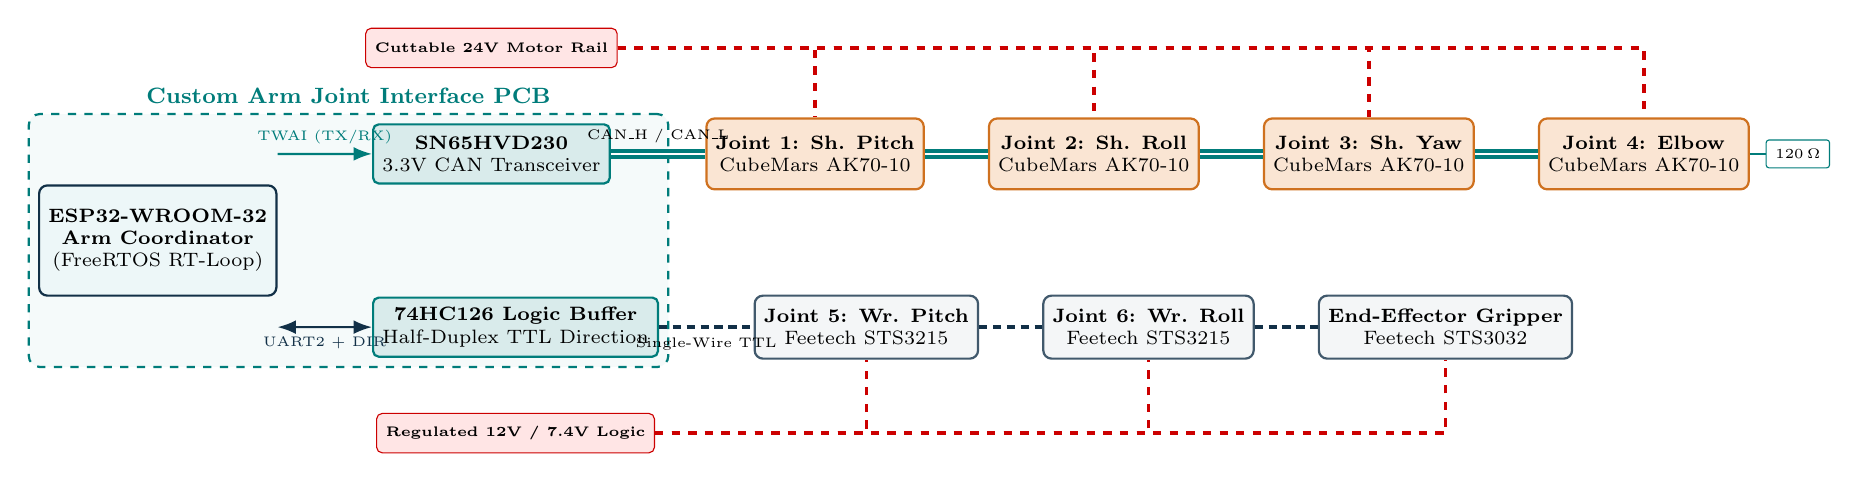
\begin{tikzpicture}[
    node distance=0.7cm and 1.1cm,
    >=Latex,
    every node/.style={font=\scriptsize, align=center},
    mcu_node/.style={draw=navy, fill=sky!50, rounded corners=3pt, thick, minimum width=2.8cm, minimum height=1.4cm},
    ic_node/.style={draw=teal, fill=teal!15, rounded corners=2pt, thick, minimum width=2.4cm, minimum height=0.75cm},
    act_qdd/.style={draw=orange!90!black, fill=orange!20, rounded corners=3pt, thick, minimum width=2.3cm, minimum height=0.9cm},
    act_servo/.style={draw=navy!80, fill=pale, rounded corners=3pt, thick, minimum width=2.3cm, minimum height=0.8cm},
    pwr_rail/.style={draw=red!80!black, fill=red!10, rounded corners=2pt, font=\bfseries\tiny, minimum width=2.2cm, minimum height=0.5cm},
    bus_can/.style={draw=teal, line width=1.4pt, double},
    bus_ttl/.style={draw=navy, line width=1.3pt, densely dashed},
    pwr_line/.style={draw=red!80!black, line width=1.2pt, dashed}
]

  % Coordinator MCU
  \node[mcu_node] (esp32) {\textbf{ESP32-WROOM-32}\\\textbf{Arm Coordinator}\\(FreeRTOS RT-Loop)};

  % Hardware ICs on Custom PCB
  \node[ic_node, right=1.2cm of esp32, yshift=1.1cm] (can_xcvr) {\textbf{SN65HVD230}\\3.3V CAN Transceiver};
  \node[ic_node, right=1.2cm of esp32, yshift=-1.1cm] (ttl_buffer) {\textbf{74HC126 Logic Buffer}\\Half-Duplex TTL Direction};

  % Power rails
  \node[pwr_rail, above=0.7cm of can_xcvr] (pwr_24v) {Cuttable 24V Motor Rail};
  \node[pwr_rail, below=0.7cm of ttl_buffer] (pwr_12v) {Regulated 12V / 7.4V Logic};

  % CAN QDD Chain (Joints 1 to 4)
  \node[act_qdd, right=1.2cm of can_xcvr] (qdd1) {\textbf{Joint 1: Sh. Pitch}\\CubeMars AK70-10};
  \node[act_qdd, right=0.8cm of qdd1] (qdd2) {\textbf{Joint 2: Sh. Roll}\\CubeMars AK70-10};
  \node[act_qdd, right=0.8cm of qdd2] (qdd3) {\textbf{Joint 3: Sh. Yaw}\\CubeMars AK70-10};
  \node[act_qdd, right=0.8cm of qdd3] (qdd4) {\textbf{Joint 4: Elbow}\\CubeMars AK70-10};

  % TTL Servo Chain (Joints 5, 6 & Gripper)
  \node[act_servo, right=1.2cm of ttl_buffer] (servo5) {\textbf{Joint 5: Wr. Pitch}\\Feetech STS3215};
  \node[act_servo, right=0.8cm of servo5] (servo6) {\textbf{Joint 6: Wr. Roll}\\Feetech STS3215};
  \node[act_servo, right=0.8cm of servo6] (gripper) {\textbf{End-Effector Gripper}\\Feetech STS3032};

  % Grouping Box for PCB
  \begin{scope}[on background layer]
    \node[draw=teal, fill=teal!4, rounded corners=4pt, dashed, thick, fit=(esp32) (can_xcvr) (ttl_buffer), label={[teal, font=\bfseries\footnotesize]above:Custom Arm Joint Interface PCB}] (pcb_box) {};
  \end{scope}

  % Signals between ESP32 and ICs
  \draw[->, thick, teal] ($(esp32.east)+(0,1.1)$) -- node[above, font=\tiny]{TWAI (TX/RX)} (can_xcvr.west);
  \draw[<->, thick, navy] ($(esp32.east)+(0,-1.1)$) -- node[below, font=\tiny]{UART2 + DIR} (ttl_buffer.west);

  % CAN Fieldbus Daisy Chain
  \draw[bus_can] (can_xcvr.east) -- node[above, font=\tiny]{CAN\_H / CAN\_L} (qdd1.west);
  \draw[bus_can] (qdd1.east) -- (qdd2.west);
  \draw[bus_can] (qdd2.east) -- (qdd3.west);
  \draw[bus_can] (qdd3.east) -- (qdd4.west);
  \node[draw=teal, fill=white, rounded corners=1pt, right=0.2cm of qdd4, font=\tiny] (term) {$120\,\Omega$};
  \draw[thick, teal] (qdd4.east) -- (term.west);

  % Half-Duplex TTL Daisy Chain
  \draw[bus_ttl] (ttl_buffer.east) -- node[below, font=\tiny]{Single-Wire TTL} (servo5.west);
  \draw[bus_ttl] (servo5.east) -- (servo6.west);
  \draw[bus_ttl] (servo6.east) -- (gripper.west);

  % Power Connections
  \draw[pwr_line] (pwr_24v.east) -| (qdd1.north);
  \draw[pwr_line] (pwr_24v.east) -| (qdd2.north);
  \draw[pwr_line] (pwr_24v.east) -| (qdd3.north);
  \draw[pwr_line] (pwr_24v.east) -| (qdd4.north);

  \draw[pwr_line] (pwr_12v.east) -| (servo5.south);
  \draw[pwr_line] (pwr_12v.east) -| (servo6.south);
  \draw[pwr_line] (pwr_12v.east) -| (gripper.south);

\end{tikzpicture}%
}
\caption{Arm hybrid actuation and dual-bus control topology. The ESP32-WROOM-32 coordinator simultaneously drives the 1~Mbps differential CAN bus (controlling four CubeMars AK70-10 QDD actuators) and a 1~Mbps half-duplex serial TTL line (controlling two Feetech STS3215 wrist servos and the STS3032 gripper servo).}
\label{fig:arm_bus_topology}
\end{figure}

\subsection{End-Effector: 2-Finger Parallel Gripper}
\label{subsec:end_effector}
Both arms terminate in a lightweight, modular 2-finger parallel-jaw gripper engineered for everyday object manipulation.

\subsubsection{Mechanics and Linear Stroke}
The gripper mechanism utilizes a symmetrical dual-rack-and-pinion transmission driven directly by a Feetech STS3032 compact serial bus servo ($7.4\text{V}$, $4.5\text{ N}\cdot\text{m}$ stall torque). The pinion engages two opposing hardened nylon racks guiding the fingers along miniature stainless steel linear rails, delivering a linear jaw stroke of:
\begin{equation}
  S_{\text{stroke}} = 0\text{--}85\text{ mm},
\end{equation}
with a full closing duration of $t_{\text{close}} \approx 0.35\text{ s}$. The $85\text{ mm}$ stroke accommodates the vast majority of domestic items, including drinking glasses, bottles, food cans, fruits, and small boxes.

\subsubsection{Compliant Silicone Gripping Pads}
The rigid 3D-printed fingers (Carbon-Fiber Reinforced PETG) are fitted with modular, vulcanized silicone pads featuring high-friction herringbone tread patterns ($\mu_{\text{friction}} \ge 0.85$ on dry glass/metal). The compliant silicone layer ($3\text{ mm}$ thickness, Shore 40A durometer) passively conforms to curved and irregular workpiece geometries, distributing contact pressures and preventing object slippage under dynamic arm accelerations.

\subsubsection{Current-Based Grasp Force Regulation}
The gripper achieves force-sensitive grasping without delicate external strain-gauge load cells by reading motor phase current feedback from the STS3032 servo:
\begin{equation}
  F_{\text{grip}} \approx \frac{K_{\tau,\text{servo}} \cdot I_{\text{servo}}}{r_{\text{pinion}}},
\end{equation}
where $r_{\text{pinion}} = 12\text{ mm}$ is the pitch radius of the drive gear. The ESP32 firmware monitors current draw at $200\text{ Hz}$. Upon detecting a steep current gradient indicating object contact, the controller clamps jaw motion to a programmable force setpoint ($F_{\text{target}} \in [5\text{ N}, 25\text{ N}]$), preventing the crushing of fragile objects (e.g., disposable plastic cups or ripe fruit).

\subsection{Subsystem 5: Active Perception Head and Neck Device}
\label{subsec:subsystem_5_head}
The Active Perception Head acts as the visual and auditory sensory hub of the platform, supporting autonomous navigation, spatial manipulation, and human-robot dialogue.

\subsubsection{2-DoF Pan-Tilt Kinematics}
The head assembly is mounted atop the torso mast via a 2-DoF active pan-tilt gimbal mechanism driven by two Feetech STS3215 12V serial bus servos ($2.9\text{ N}\cdot\text{m}$ stall torque). The kinematic range provides:
\begin{itemize}[leftmargin=1.5em]
  \item \textbf{Pan Axis:} $\theta_{\text{pan}} \in [-90^\circ, +90^\circ]$ (horizontal azimuthal sweep).
  \item \textbf{Tilt Axis:} $\theta_{\text{tilt}} \in [-45^\circ, +30^\circ]$ (downward workspace inspection to upward face tracking).
\end{itemize}
Because the entire sensor head payload (camera, microphones, speaker, and housing) weighs less than $450\text{ g}$, the STS3215 servos operate far below their thermal limits, achieving slew velocities up to $180^\circ/\text{s}$ for rapid saccadic gaze shifts.

\subsubsection{Vision and Acoustic Transducers}
\begin{itemize}[leftmargin=1.5em]
  \item \textbf{Intel RealSense RGB-D Camera:} Streams active infrared stereo depth ($1280 \times 720$ at 30~fps) and full-color RGB frames via a USB~3.0 link directly to the Jetson Orin NX host. Operating over a range of $0.2\text{--}3.0\text{ m}$, it feeds both the 3D voxel TSDF reconstruction pipeline and the VLA policy visual encoder.
  \item \textbf{ReSpeaker 2-Mic Pi HAT Array:} Incorporates dual omnidirectional microphones with an onboard stereo codec. Features hardware-accelerated acoustic echo cancellation (AEC) and Time-Difference-of-Arrival (TDOA) sound localization, allowing the head to turn autonomously toward speaking humans.
  \item \textbf{2W Broad-Dispersion Speaker:} Driven by an onboard I2S Class-D audio amplifier, delivering clear synthesized speech dialogue, task feedback, and audible emergency alarms.
\end{itemize}

\subsubsection{Custom Head Interface PCB}
An ESP32-WROOM-32 DevKitC and a Custom Head Interface PCB manage local pan-tilt servo commands, decode I2S audio streams, and drive an external addressable RGB LED indicator ring (displaying robot emotional state and system operational modes).

\subsection{Subsystem 6: Power Distribution and Safety Subsystem}
\label{subsec:subsystem_6_power}
The Power Distribution and Safety Subsystem delivers clean, protected electrical energy across all active platform devices while enforcing fail-safe hardware disconnection.

\subsubsection{Battery Chemistry and Energy Capacity}
The primary electrical power source is a high-energy-density 24V, 20Ah Lithium Iron Phosphate (LiFePO$_4$) battery pack ($\sim 480\text{ Wh}$ nominal energy storage). Compared to standard Lithium-Ion (NMC) cells, LiFePO$_4$ chemistry offers superior thermal runaway resistance (thermal threshold $>270^\circ\text{C}$), an extended operational cycle life ($>2000$ cycles at $80\%$ DoD), and high continuous discharge capability ($2\text{C} = 40\text{A}$). 

At a nominal continuous platform power draw of $115\text{ W}$ (35W compute + 30W idle actuators + 50W base transit), the $480\text{ Wh}$ pack guarantees an uninterrupted operational runtime of:
\begin{equation}
  t_{\text{runtime}} = \frac{480\text{ Wh} \cdot 0.85}{115\text{ W}} \approx 3.55\text{ hours},
\end{equation}
fully fulfilling Requirement~E02. The pack is paired with a dedicated 24V, 5A LiFePO$_4$ profile smart charger providing full recharge in approximately $4\text{ hours}$.

\subsubsection{Galvanic Partitioning and Synchronous DC-DC Regulation}
To eliminate ground loops and prevent actuator electromagnetic interference (EMI) from corrupting high-speed digital buses, power distribution is split across two architecturally separated domains:
\begin{enumerate}[leftmargin=1.5em]
  \item \textbf{Protected Logic Rail (Uncuttable 24V):} Feeds three high-efficiency ($>94\%$) synchronous buck regulators:
  \begin{itemize}
    \item $24\text{V} \to 19\text{V}$ ($6\text{A}$, $114\text{W}$ max): Supplies regulated power to the NVIDIA Jetson Orin NX host.
    \item $24\text{V} \to 12\text{V}$ ($10\text{A}$, $120\text{W}$ max): Powers the Feetech serial bus servos, audio amplifiers, and cooling blowers.
    \item $24\text{V} \to 5\text{V}$ ($10\text{A}$, $50\text{W}$ max): Supplies the distributed ESP32 microcontrollers, IMU, ultrasonic sensors, and LiDAR motor.
  \end{itemize}
  \item \textbf{Switched Motor Power Rail (Cuttable 24V):} Supplies raw battery voltage directly to the 9$\times$ CubeMars AK70-10 QDD actuators and the dual base BLDC gearmotors through a heavy-duty 24V, 40A continuous safety contactor relay.
\end{enumerate}

\subsubsection{Hardware Emergency Stop (E-Stop) Disconnect Circuit}
Operational safety compliance (ISO~13482~\cite{iso13482}) is guaranteed via a dedicated, hardwired dual-channel safety circuit. A red latching mushroom E-Stop push-button is mounted prominently on the upper torso spine, wired in series with an optional wireless safety receiver. Depressing the E-Stop button breaks the coil circuit of the 40A safety contactor. Spring-loaded mechanical contacts disconnect the motor power rail in:
\begin{equation}
  t_{\text{disconnect}} \le 8\text{ ms} \ll 10\text{ ms} \quad (\text{Requirement E03}).
\end{equation}
Because the logic rail bypasses the contactor, compute, perception, wireless telemetry, and system diagnostic logs remain fully energized, allowing the robot to transmit immediate fault diagnostics without losing system state.

\subsection{Subsystem 7: Central Compute and Communications}
\label{subsec:subsystem_7_compute}
Subsystem~7 centralizes high-level artificial intelligence inference, real-time trajectory generation, and multi-interface communications.

\subsubsection{Primary Edge Compute: NVIDIA Jetson Orin NX 16 GB}
High-level computational processing is performed by an NVIDIA Jetson Orin NX module (16~GB 128-bit LPDDR5 RAM, 1024-core NVIDIA Ampere architecture GPU with 32 Tensor Cores, and an 8-core Arm Cortex-A78AE v8.2 64-bit CPU). The module delivers up to 100~TOPS of sparse INT8 AI performance, comfortably accommodating parallel execution of:
\begin{itemize}[leftmargin=1.5em]
  \item Quantized multimodal VLA models (OpenVLA / $\pi_0$) running via TensorRT-LLM at $5\text{--}10\text{ Hz}$.
  \item Real-time 3D Signed Distance Field (SDF) voxel mapping and depth-point registration.
  \item 2D SLAM and MPPI local trajectory generation at $50\text{ Hz}$.
\end{itemize}

\subsubsection{Operating System and Real-Time Scheduling Architecture}
The host runs Ubuntu 22.04 LTS (JetPack 6) patched with the PREEMPT\_RT real-time kernel. To eliminate thread contention and scheduling jitter, computational resources are partitioned using Linux Control Groups (\texttt{cgroups}) and CPU core affinity pinning:
\begin{itemize}[leftmargin=1.5em]
  \item \textbf{Cores 0--1 (Real-Time Middleware):} Isolated from standard Linux scheduling; dedicated exclusively to \texttt{ros2\_control}, fieldbus CAN I/O threads, and the $200\text{ Hz}$ state estimation UKF running under \texttt{SCHED\_FIFO} priority.
  \item \textbf{Cores 2--5 (Mission Autonomy):} Executes Nav2 costmap processing, MoveIt~2 collision checking, and BehaviorTree.CPP evaluation.
  \item \textbf{Cores 6--7 (Background Services):} Hosts the web server, WebRTC streaming pipeline, rosbridge WebSocket endpoints, and system logging.
\end{itemize}

\subsubsection{Communication Gateways and Network Infrastructure}
\begin{itemize}[leftmargin=1.5em]
  \item \textbf{Isolated USB-to-CAN Gateway:} Connects the Jetson host to the platform's primary 1~Mbps CAN bus, featuring optical galvanic isolation ($2.5\text{ kV}_{\text{RMS}}$) and hardware message timestamping ($<10\ \mu\text{s}$).
  \item \textbf{Industrial Gigabit Network Switch:} Routes internal 1000BASE-T Ethernet between the Jetson host, external torso bulkhead RJ-45 service ports, and high-speed telemetry bridges.
  \item \textbf{Dual-Band Wi-Fi 6 \& Bluetooth 5.2:} Provides high-throughput, low-latency wireless communication ($>600\text{ Mbps}$) for remote browser-based teleoperation, cloud fleet management, and remote software deployment.
\end{itemize}

\subsection{Subsystem 8: HMI, Web Dashboard, and Task Port Gateway}
\label{subsec:subsystem_8_hmi}
The Human-Machine Interface (HMI) establishes intuitive physical, browser-based, and algorithmic interfaces for operating and programming the semi-humanoid robot.

\subsubsection{Physical Torso Panel and Bulkhead Ports}
Mounted on the front and rear of the upper torso housing, the physical panel provides immediate local diagnostics and field service access:
\begin{itemize}[leftmargin=1.5em]
  \item \textbf{5--7'' Touchscreen Status Display:} Presents high-contrast system telemetry, including current Wi-Fi SSID and assigned IP address, battery State of Charge (SoC\%), active ROS~2 node states, actuator temperatures, and active error codes.
  \item \textbf{Bulkhead Programming and Service Bay:} Features an industrial RJ-45 Gigabit Ethernet port, dual high-speed USB~3.0 service ports, a keyed master power switch, and a soft reboot button. This allows developers to flash microcontrollers, extract flight-recorder logs, and deploy software updates without dismantling chassis panels.
\end{itemize}

\subsubsection{Browser Web Dashboard and Teleoperation Console}
Remote teleoperation and fleet monitoring are conducted via a responsive, single-page web dashboard developed using React, TypeScript, and TailwindCSS, communicating with the robot over WebRTC and WebSocket links:
\begin{itemize}[leftmargin=1.5em]
  \item \textbf{Low-Latency Teleoperation Console:} Streams low-latency ($<80\text{ ms}$) H.264 video from the RealSense camera via WebRTC. Operators can command mobile base translation and arm end-effector Cartesian jogging using virtual on-screen joysticks, standard keyboard hotkeys, or USB game controllers (via the HTML5 Gamepad API).
  \item \textbf{Diagnostic Alarm Console:} Displays real-time visual alerts and audible warnings upon anomalous hardware states, such as actuator overtemperature ($T > 75^\circ\text{C}$), fieldbus packet loss, battery under-voltage ($\text{SoC} < 15\%$), or LiDAR point cloud occlusion.
  \item \textbf{Interactive Task Programming (Macro Waypoint Recorder):} Enables non-expert operators to program complex mobile manipulation tasks graphically. The interface features a record-and-playback macro recorder: operators lead the compliant arm through a sequence of waypoints, save Cartesian and gripper states as named skills, and link them into executable behavior tree routines.
\end{itemize}

\subsubsection{Task Port Gateway: Decoupled ROS 2 Action Servers}
The Task Port Gateway implements the software isolation boundary described in Section~\ref{sec:system_architecture}. It encapsulates low-level hardware complexity behind standardized ROS~2 Action servers:
\begin{itemize}[leftmargin=1.5em]
  \item \textbf{Navigation Action:} \texttt{/navigate\_to\_pose} dispatches $SE(2)$ goals to Nav2 (action type: \texttt{NavigateToPose}).
  \item \textbf{Manipulation Actions:} \texttt{/pick\_object} and \texttt{/place\_object} command grasp and placement routines (action type: \texttt{PickObject}).
  \item \textbf{Autonomous Docking Action:} \texttt{/dock\_robot} coordinates contact engagement with the dock (action type: \texttt{Dock}).
\end{itemize}
By forcing all cognitive models and external software pipelines to interact strictly through these typed Action endpoints, the Task Port Gateway guarantees that unexpected high-level crashes or network disconnects never jeopardize the physical integrity of the platform.

\section{Cross-Domain Engineering Allocation}
\label{sec:domain_allocation}

\subsection{Multidisciplinary Allocation Framework (VDI 2206)}
The realization of an autonomous mobile manipulator demands a rigorous departure from fragmented, discipline-isolated development methodologies. In conventional engineering workflows, the mechanical skeleton, electrical power grid, motor actuation, and software intelligence are frequently addressed in consecutive isolation. For high-degree-of-freedom cyber-physical systems (CPS), this serialized paradigm routinely induces structural inefficiencies, thermal runaway at motor joints, communication bus saturation, and costly redesign iterations. 

To systematically overcome these failure modes, the system-level conceptual requirements ($R_1$--$R_{24}$) and tripartite flow structures ($\mathbf{M}$, $\mathbf{E}$, $\mathbf{I}$) formulated in Section~\ref{sec:functional_structure} are translated into domain-specific engineering work packages in strict accordance with the VDI~2206 design methodology~\cite{vdi2206}. Operating across the descending and ascending branches of the VDI~2206 V-model, the platform architecture establishes a synchronized triad across three primary engineering domains:
\begin{enumerate}[leftmargin=1.5em]
  \item \textbf{Mechanical Engineering:} Structural chassis, kinematics linkages, mass/inertia distribution, thermal heat sinking, and environmental ingress protection.
  \item \textbf{Electrical \& Embedded Engineering:} High-current power distribution, Li-ion battery management, safety interlocks, custom PCB design, and hard real-time motor commutation firmware.
  \item \textbf{Computer Science and Software Engineering:} Real-time middleware orchestration, SLAM and navigation, collision-free manipulation planning, Vision-Language-Action (VLA) foundation models, and human-machine teleoperation interfaces.
\end{enumerate}

Table~\ref{tab:domain_allocation_matrix} formalizes the domain allocation matrix, detailing the division of responsibilities, primary work packages, concrete deliverables, and quantifiable verification metrics across the platform lifecycle.

\begin{small}
\begin{longtable}{@{}p{0.13\textwidth} p{0.22\textwidth} p{0.23\textwidth} p{0.18\textwidth} p{0.13\textwidth}@{}}
\caption{Formal VDI 2206 cross-domain engineering allocation matrix for the semi-humanoid platform.}
\label{tab:domain_allocation_matrix}\\
\toprule
\textbf{Domain} & \textbf{Work Package (WP)} & \textbf{Scope \& Key Responsibilities} & \textbf{Primary Deliverables} & \textbf{Verification Metric} \\
\midrule
\endfirsthead
\multicolumn{5}{c}{{\bfseries Table \thetable\ continued from previous page}} \\
\toprule
\textbf{Domain} & \textbf{Work Package (WP)} & \textbf{Scope \& Key Responsibilities} & \textbf{Primary Deliverables} & \textbf{Verification Metric} \\
\midrule
\endhead
\midrule
\multicolumn{5}{r}{{Continued on next page\dots}} \\
\bottomrule
\endfoot
\bottomrule
\endlastfoot

\textbf{Mechanical} & 
WP-ME1: Base Drivetrain \& Structural Chassis & 
Differential chassis frame, motor mounts, wheel hubs, ground clearance ($>30\text{ mm}$), and caster suspension. & 
3D CAD assembly, structural FEA stress reports, CNC fabrication drawings. & 
Factor of safety $S_f \ge 2.2$; payload $\ge 80\text{ kg}$; chassis deflection $<0.5\text{ mm}$. \\
\addlinespace[3pt]
& 
WP-ME2: Fixed Mast Torso \& Modular Waist Axis & 
Structural fixed mast frame, CubeMars AK70-10 modular mounting, bearing load isolation, and CoM balance. & 
Torso weldment/bracket CAD, bearing load calculation sheets, physical frame. & 
Structural deflection $<0.5\text{ mm}$; modular waist moment load $\ge 45\text{ N}\cdot\text{m}$. \\
\addlinespace[3pt]
& 
WP-ME3: Dual 6-DoF Manipulator Kinematic Chain & 
Shoulder, elbow, and wrist linkages, link inertia reduction, carbon-fiber / aluminum structural tubes, cable passages. & 
Parametric arm CAD, mass/inertia matrices ($I_{xx}, I_{yy}, I_{zz}$), 3D printed / machined links. & 
Natural frequency $\omega_n \ge 18\text{ Hz}$; settling time $t_s \le 0.4\text{ s}$; arm payload $\ge 2.0\text{ kg}$. \\
\addlinespace[3pt]
& 
WP-ME4: Modular End-Effectors \& 2-DoF Neck & 
Parallel-jaw grippers with silicone contact pads, 2-DoF pan-tilt sensor head housing RGB-D camera and microphones. & 
Gripper CAD with ISO~9409-1 flange, pan-tilt head gimbal assembly, 3D MJF PA12 parts. & 
Clamping force $15\text{--}35\text{ N}$; grasp span $0\text{--}85\text{ mm}$; head pan $\pm 90^\circ$, tilt $+45^\circ/-30^\circ$. \\
\midrule

\textbf{Electrical \&} & 
WP-EE1: Power Subsystem \& Safety Interlocks & 
$24\text{V}$, $20\text{Ah}$ $\text{LiFePO}_4$ battery integration, BMS, main 40~A contactor, E-Stop disconnect loop, and multi-rail DC-DC. & 
Power schematic, wiring harness pinout diagrams, battery enclosure, safety contactor board. & 
E-Stop disconnect latency $\le 10\text{ ms}$; voltage ripple $<1.5\%$; battery run-time $\ge 4.0\text{ h}$. \\
\addlinespace[3pt]
\textbf{Embedded} & 
WP-EE2: Custom Subsystem PCB Design & 
Design and population of 4 custom boards: Base Controller, Power/Waist, Head Interface, and Dual Arm Joint Interface. & 
KiCad schematics, multi-layer Gerber files, assembled and bench-tested PCBs. & 
$100\%$ net continuity; CAN bus termination $120\,\Omega \pm 1\%$; 40~A trace thermal rise $<25^\circ\text{C}$. \\
\addlinespace[3pt]
& 
WP-EE3: Real-Time Embedded Firmware & 
Firmware for 5x ESP32-WROOM-32 MCUs, TWAI CAN drivers, CiA~402 drive state machines, half-duplex TTL servo chains. & 
C/C++ FreeRTOS firmware repositories, micro-ROS client nodes, flash automation scripts. & 
Deterministic loop rate $1\text{ kHz}$; CAN packet transmission jitter $<150\,\mu\text{s}$; zero watchdog timeouts. \\
\addlinespace[3pt]
& 
WP-EE4: Signal Conditioning \& Harnessing & 
Quadrature encoder decoding, 9-DoF IMU SPI acquisition, ultrasonic ranging, continuous-rotation wire shielding. & 
Finished wiring harnesses with strain relief, ferrite choke clamp documentation. & 
EMI noise margin $>20\text{ dB}$; zero dropped encoder pulses up to $3000\text{ RPM}$; IMU rate $\ge 200\text{ Hz}$. \\
\midrule

\textbf{Software \&} & 
WP-CS1: Compute Infrastructure \& RTOS Middleware & 
NVIDIA Jetson Orin NX OS setup, PREEMPT\_RT real-time Linux kernel, ROS~2 Jazzy infrastructure, micro-ROS agent. & 
Custom Linux rootfs image, Docker deployment containers, ros2\_control hardware interfaces. & 
Kernel interrupt latency $\le 50\,\mu\text{s}$; inter-process zero-copy transport latency $<100\,\mu\text{s}$. \\
\addlinespace[3pt]
\textbf{Computer} & 
WP-CS2: Autonomous Base Navigation \& SLAM & 
2D LiDAR SLAM, costmap generation, dynamic obstacle avoidance, and Nav2 path tracking controllers. & 
Nav2 configuration packages, customized costmap plugins, AMCL tuning parameters. & 
Global localization error $\le 30\text{ mm}$, heading error $\le 2.0^\circ$; transit speed $0.8\text{--}1.0\text{ m/s}$. \\
\addlinespace[3pt]
\textbf{Science} & 
WP-CS3: Manipulation Kinematics \& Dual-Arm Planning & 
MoveIt~2 integration, bio-IK / TRAC-IK inverse kinematics solvers, collision-free Cartesian trajectory generation. & 
MoveIt~2 configuration packages, dual-arm collision models, self-collision avoidance matrices. & 
IK solve time $\le 5\text{ ms}$; Cartesian trajectory execution repeatability $\le \pm 2.0\text{ mm}$. \\
\addlinespace[3pt]
& 
WP-CS4: Standardized Task Port \& Safety Supervisor & 
Action servers exposing decoupled task primitives (/navigate\_to\_pose, /pick\_object), runtime safety state observer. & 
ROS~2 Action Server packages, ISO~13482 safety monitoring node, Python client verification scripts. & 
Task dispatch latency $\le 25\text{ ms}$; safety override reaction time $\le 20\text{ ms}$; 100\% command isolation. \\
\addlinespace[3pt]
& 
WP-CS5: Multimodal Perception \& VLA Integration & 
RealSense RGB-D point cloud segmentation, Whisper speech recognition, OpenVLA foundation policy trajectory streaming. & 
Perception ROS~2 nodes, Whisper STT inference pipeline, OpenVLA action chunking adapter. & 
Object pose estimation rate $\ge 15\text{ Hz}$; VLA action inference rate $\ge 10\text{ Hz}$; speech response $<1.2\text{ s}$. \\
\addlinespace[3pt]
& 
WP-CS6: Web Teleoperation \& Fleet Telemetry & 
Browser-based dashboard providing real-time video streaming, 3D LiDAR point cloud display, and joint teleoperation. & 
Full-stack web application (React, WebRTC, rosbridge\_suite WebSocket server). & 
Glass-to-glass video streaming latency $\le 120\text{ ms}$; telemetry update rate $\ge 20\text{ Hz}$. \\
\end{longtable}
\end{small}

\subsection{Domain Work Packages, Primary Deliverables, and Verification Metrics}

\subsubsection{Mechanical Engineering Domain}
The mechanical engineering team holds primary ownership over the structural integrity, kinematics geometry, payload capacity, and mass properties of the robotic system:
\begin{itemize}[leftmargin=1.5em]
  \item \textbf{Chassis and Drivetrain (WP-ME1):} Responsible for the structural baseplate machined from $6\text{ mm}$ 6061-T6 aluminum alloy. The chassis houses two 100~W brushed DC gearmotors driving $\varnothing 200\text{ mm}$ high-traction rubber wheels, paired with dual $100\text{ mm}$ heavy-duty polyurethane swivel casters. Finite element analysis (FEA) validates that under a combined static and dynamic payload of $85\text{ kg}$, von Mises stresses remain well below the yield strength ($\sigma_{\text{yield}} = 276\text{ MPa}$), yielding a safety factor $S_f \ge 2.2$.
  \item \textbf{Fixed Mast Torso Structure and Waist Axis (WP-ME2):} The baseline torso adopts a rigid structural fixed mast constructed from modular $30 \times 30\text{ mm}$ aluminum extrusions, delivering the invariant 18-DoF baseline. To support the modular torso articulation path budgeted in the BOM, it incorporates precision mounting provisions and dual angular contact ball bearings for a CubeMars AK70-10 QDD waist tilt actuator, isolating the gearbox from parasitic radial and axial moment loads during forward reaches.
  \item \textbf{Dual 6-DoF Manipulators (WP-ME3):} Each 6-DoF arm is configured with four proximal CubeMars AK70-10 QDD actuators (shoulder pitch, shoulder roll, shoulder yaw, elbow pitch) and two distal Feetech STS3215 serial bus servos (wrist pitch, wrist roll). Structural links are engineered using thin-walled aluminum tubing and hollow carbon-fiber composite sections, minimizing link mass while shifting structural resonance frequencies above $18\text{ Hz}$ to avoid control-loop excitation.
  \item \textbf{Modular End-Effector and Head Assembly (WP-ME4):} The parallel-jaw gripper uses a compact Feetech STS3032 bus servo driving a dual-rack-and-pinion transmission. Gripper jaws feature exchangeable shore-A 60 silicone pads optimized for domestic tableware grasping ($0\text{--}85\text{ mm}$ opening span). The perception head provides 2-DoF pan/tilt articulation driven by dual Feetech STS3215 servos, carrying the Intel RealSense depth camera and microphone array.
  \item \textbf{Optional Prismatic Column (WP-ME5):} When installed as a modular add-on, the telescopic column utilizes a 24~V electric linear actuator ($300\text{ mm}$ stroke, $1500\text{ N}$ static thrust) guided by dual precision recirculating ball linear guide rails (MGN15 series), completely decoupling moment loads from the actuator lead screw.
\end{itemize}

\subsubsection{Electrical and Embedded Engineering Domain}
The electrical engineering team manages the complete energy transformation pipeline, power conditioning, circuit design, and distributed real-time microcontroller network:
\begin{itemize}[leftmargin=1.5em]
  \item \textbf{Power Architecture and Energy Storage (WP-EE1):} The primary energy source is an $8\text{S}$, $24\text{V}$, $20\text{Ah}$ $\text{LiFePO}_4$ battery pack ($\sim 480\text{ Wh}$) with an internal Battery Management System (BMS) supporting continuous $40\text{A}$ discharge and $100\text{A}$ transient pulse capability. A 40~A continuous-duty safety contactor provides galvanically isolated hardware power cutoff.
  \item \textbf{Custom PCB Hardware Development (WP-EE2):} To eliminate cabling rats-nests and mitigate ground loops, four custom populated PCBs are developed:
  \begin{enumerate}[leftmargin=1.2em]
    \item \emph{Custom Base Controller PCB:} Combines an ESP32 carrier, dual-channel H-bridge motor driver (40~V / 15~A per channel), optical encoder quadrature counters, and ultrasonic sensor headers.
    \item \emph{Custom Power Distribution \& Waist PCB:} Houses high-current fused battery busbars, three high-efficiency synchronous buck converters ($24\text{V} \rightarrow 19\text{V } 4\text{A}$, $24\text{V} \rightarrow 12\text{V } 6\text{A}$, and $24\text{V} \rightarrow 5\text{V } 5\text{A}$), a 3.3~V CAN transceiver (SN65HVD230) interfaced to the ESP32 Two-Wire Automotive Interface (TWAI), and safety relay coil drivers.
    \item \emph{Custom Head Interface PCB:} Integrates half-duplex TTL bus servo level shifters, an I2S stereo class-D audio power amplifier ($2 \times 3\text{ W}$), microphone breakout headers, and an ESP32 carrier.
    \item \emph{Custom Arm Joint Interface PCBs (x2):} Mounted at each shoulder base, each board integrates a 3.3~V CAN transceiver on the ESP32 TWAI bus (interfacing the 4x AK70-10 QDD chain) and a 74HC126-based half-duplex TTL buffer circuit (interfacing the 2x wrist servos and 1x gripper servo).
  \end{enumerate}
  \item \textbf{Distributed Real-Time Firmware (WP-EE3):} Five ESP32-WROOM-32 microcontrollers execute FreeRTOS firmware. Low-level control tasks operate deterministically:
  \begin{itemize}
    \item Base MCU: Executes closed-loop PID velocity tracking ($100\text{ Hz}$) using quadrature encoder feedback.
    \item Torso MCU: Reads 9-DoF IMU data via SPI ($200\text{ Hz}$), executes waist angle trajectory interpolation, and monitors battery bus voltages.
    \item Arm MCUs (x2): Translates high-level joint trajectory setpoints into 1~kHz CAN command frames dispatched to the CubeMars AK70-10 FOC inverters and 50~Hz serial packets dispatched to the Feetech bus servos.
    \item Head MCU: Regulates pan/tilt tracking angles and manages audio input/output buffers.
  \end{itemize}
  \item \textbf{Signal Integrity and Harnessing (WP-EE4):} Critical communication lines (CAN, UART, I2S) are routed through twisted shielded pairs with common-mode choke filtering to maintain robust signal margins in the vicinity of pulse-width modulated (PWM) motor power lines.
\end{itemize}

\subsubsection{Computer Science and Software Engineering Domain}
The software engineering team owns the high-level computational pipelines, real-time operating system middleware, spatial navigation, manipulation planning, and physical AI execution:
\begin{itemize}[leftmargin=1.5em]
  \item \textbf{Operating System and Middleware Core (WP-CS1):} The NVIDIA Jetson Orin NX (16~GB) executes Ubuntu 24.04 LTS patched with the PREEMPT\_RT real-time kernel. The core communication layer runs ROS~2 Jazzy Jalisco. Fast DDS serves as the default middleware implementation, configured with shared-memory (SHM) intra-host transport to achieve sub-$100\,\mu\text{s}$ message transfer latencies for high-bandwidth RGB-D point clouds.
  \item \textbf{Autonomous Navigation Stack (WP-CS2):} Implements the Nav2 framework~\cite{nav2}. Planar range data from the Slamtec RPLiDAR A1M8 ($360^\circ$ FoV, 12~m range) is fused with wheel odometry and torso IMU data using an Extended Kalman Filter (EKF) via the \texttt{robot\_localization} node. Nav2 manages layered 2D costmaps, obstacle inflation, and dynamic obstacle avoidance using the Regulated Pure Pursuit (RPP) controller.
  \item \textbf{Dual-Arm Manipulation Planning (WP-CS3):} The MoveIt~2 framework~\cite{moveit2} manages kinematic planning for the dual 6-DoF arms and waist axis. The kinematic models enforce joint limits, velocity bounds, and dynamic obstacle clearance. Self-collision avoidance matrices are precomputed across the robot URDF model to guarantee that arm-to-arm and arm-to-torso collision-free paths are generated within $\le 5\text{ ms}$.
  \item \textbf{Standardized Task Port Layer (WP-CS4):} Encapsulates all robotic capabilities into standardized ROS~2 Action Servers. The application layer commands actions via high-level goal definitions without access to raw motor registers or microcontroller buses, enforcing strict interface decoupling.
  \item \textbf{Perception, Speech, and Foundation AI (WP-CS5):} The perception pipeline performs point cloud filtering, plane extraction, and Euclidean cluster extraction for tabletop object segmentation. Real-time automatic speech recognition is performed locally using an optimized INT8 quantized Whisper model. For autonomous manipulation, the OpenVLA foundation model~\cite{openvla} processes head camera RGB frames and natural language instructions to predict 7-DoF end-effector delta action sequences.
  \item \textbf{Web Teleoperation Dashboard (WP-CS6):} A responsive web application developed in React communicates with ROS~2 via \texttt{rosbridge\_suite} WebSockets. Low-latency H.264 video streams from the RealSense camera are relayed via WebRTC, enabling real-time remote monitoring, emergency stop triggering, and manual teleoperation.
\end{itemize}

\subsection{Cross-Domain Interface Management}
In complex mechatronic systems, physical and operational failures predominantly manifest at domain boundaries. Rigorous cross-domain interface management is therefore essential to prevent integration bottlenecks.

\subsubsection{Physical Mounting Standards}
Mechanical interfaces across subsystems conform to established international robotics standards:
\begin{itemize}[leftmargin=1.5em]
  \item \textbf{End-Effector Flange:} Both wrist tool mounting plates adhere to the ISO~9409-1-50-4-M6 standard (50~mm pitch circle diameter, 4x M6 threaded holes, and $\varnothing 31.5\text{ mm}$ locating boss). This standardized interface permits rapid swapping between parallel-jaw grippers, suction cups, and custom inspection tools in under 5 minutes without mechanical redesign.
  \item \textbf{Structural Assembly Fasteners:} All structural connections utilize metric grade 8.8 and 10.9 steel fasteners (DIN 912 socket head cap screws and DIN 7991 countersunk screws) engaging precision-machined threads in aluminum alloy plates or steel threaded inserts (Helicoil / PEM).
  \item \textbf{Subsystem Quick-Disconnects:} The complete upper-body torso mounts to the mobile base chassis using an array of six M6 mounting bolts and two precision locating dowel pins (DIN 6325, $\varnothing 6\text{ mm}$ m6 tolerance), ensuring sub-$0.05\text{ mm}$ positional repeatability upon reassembly.
\end{itemize}

\subsubsection{Electrical Voltage Domains and Power Routing}
To isolate high-energy motor commutation noise from sensitive logic and computing circuitry, the power architecture enforces four segregated voltage domains:
\begin{enumerate}[leftmargin=1.5em]
  \item \textbf{Raw Battery Bus ($24.0\text{--}29.2\text{V}$, High Power):} Supplies the CubeMars AK70-10 QDD motor drives (shoulder, elbow, waist) and the dual 100~W differential base drive motors. Protected by a 40~A main fuse and safety contactor.
  \item \textbf{Regulated 19~V Domain ($19.0\text{V} \pm 1.5\%$, 4.0~A Continuous):} Dedicated exclusively to the NVIDIA Jetson Orin NX compute module, derived via an isolated synchronous buck converter.
  \item \textbf{Regulated 12~V Domain ($12.0\text{V} \pm 2.0\%$, 6.0~A Continuous):} Powers the Feetech STS3215/STS3032 serial bus servos (wrists, grippers, pan/tilt head) and the Intel RealSense depth sensor.
  \item \textbf{Regulated 5~V \& 3.3~V Domains (Low Power Logic):} Powers the Slamtec RPLiDAR, ReSpeaker microphone array, ESP32 microcontrollers, CAN transceivers, and digital sensor pull-ups.
\end{enumerate}
All subsystem grounds converge at a single central star-ground point located on the main power distribution board, mitigating ground potential differentials and eliminating closed ground loops.

\subsubsection{Communication Protocols and Fieldbus Determinism}
The communication architecture maps data flows to appropriate protocols based on required bandwidth and latency constraints:
\begin{itemize}[leftmargin=1.5em]
  \item \textbf{High-Speed Cognitive Bus (Gigabit Ethernet / USB 3.0):} Carries high-bandwidth sensory data (uncompressed $1280 \times 720$ @ 30~fps RGB-D video streams and raw point clouds) between the Intel RealSense camera and the NVIDIA Jetson Orin NX host.
  \item \textbf{System Fieldbus (CAN 2.0B / TWAI):} Connects the Jetson compute host to the distributed ESP32 microcontrollers and CubeMars AK70-10 motor actuators at 1~Mbps. Motor setpoints and telemetry packets operate at a cyclic rate of 1~kHz with packet jitter constrained below $150\,\mu\text{s}$.
  \item \textbf{Subsystem Device Serial Buses (Half-Duplex Asynchronous TTL):} Distributes position commands and reads position/temperature telemetry from the Feetech STS3215/STS3032 serial servos at 1~Mbps using custom multi-drop single-wire UART transceivers.
  \item \textbf{Sensor Peripheral Buses (SPI / I2C / I2S):} Dedicated local buses connecting microcontrollers to peripheral sensors: SPI at 10~MHz for the BNO085 9-DoF IMU, I2S for high-fidelity digital audio input/output, and GPIO interrupt lines for hardware limit switches.
\end{itemize}

\subsubsection{Safety Interlocks and Fault Isolation}
The platform enforces a layered safety architecture in compliance with ISO~13482 personal care robotics standards~\cite{iso13482}:
\begin{itemize}[leftmargin=1.5em]
  \item \textbf{Hardware Safety Interlock (Level 0):} A dual-channel, normally closed (NC) hardware emergency-stop loop connects the manual E-Stop pushbuttons (located on the torso shoulder and base rear) directly to the de-energizing coil of the main 40~A power contactor. Depressing the E-Stop physically severs battery power from all motor actuators within $\le 10\text{ ms}$. Crucially, the 19~V, 12~V, and 5~V logic rails remain fully energized, allowing the Jetson compute host and microcontrollers to maintain telemetry, capture event logs, and broadcast alarm states.
  \item \textbf{Firmware Watchdog Interlock (Level 1):} Each ESP32 microcontroller executes a hardware watchdog timer and monitors continuous CAN communication heartbeats from the high-level host. If communication drops for longer than $50\text{ ms}$, the local firmware automatically commands motor zero-velocity braking and disables the PWM gate drives.
  \item \textbf{Software Supervisory Interlock (Level 2):} The Task Port safety supervisor monitors Cartesian end-effector velocities, joint torque limits, and distance-to-human thresholds derived from the LiDAR and depth camera. In accordance with ISO~13482 collaborative speed and separation monitoring, the supervisor scales down platform transit speed ($v_{\text{base}} \le 0.3\text{ m/s}$) when obstacles are within $0.8\text{ m}$, and initiates a software-controlled deceleration stop if a collision trajectory is projected.
\end{itemize}

\section{Bill of Materials, Economics, and Implementation Roadmap}
\label{sec:bom_roadmap}

\subsection{Consolidated Bill of Materials (BOM)}
A foundational objective of the mechatronic design process is reconciling high-performance mobile manipulation capabilities with strict financial and procurement constraints. Grounded in the comprehensive component quotations and local Egyptian market sourcing analysis documented in the project budget evaluation, Table~\ref{tab:consolidated_bom} presents the consolidated Bill of Materials (BOM) for the complete core robotic platform.

\begin{table*}[htbp]
\centering\scriptsize
\caption{Consolidated Bill of Materials (BOM) for the core semi-humanoid robotic platform.}
\label{tab:consolidated_bom}
\begin{tabularx}{\textwidth}{@{}l Y l c r r l@{}}
\toprule
\textbf{Component} & \textbf{Technical Specification} & \textbf{Subsystem} & \textbf{Qty} & \textbf{Unit (EGP)} & \textbf{Total (EGP)} & \textbf{Category} \\
\midrule
\multicolumn{7}{@{}l}{\textbf{Actuation \& Drivetrain}} \\
DC Gearmotor with Encoder & 24V, 100W, $\sim 30:1$ planetary reduction, optical quadrature & Base & 2 & 7,405 & 14,810 & Actuation \\
QDD Actuator (AK70-10) & CubeMars AK70-10, $24.8\text{ N}\cdot\text{m}$ peak, 10:1 planetary, FOC driver & Torso, Arms & 9 & 22,155 & 199,395 & Actuation \\
Serial Bus Servo (STS3215) & Feetech STS3215, 12V, $2.9\text{ N}\cdot\text{m}$ stall, half-duplex TTL bus & Head, Arms & 6 & 1,480 & 8,880 & Actuation \\
Serial Bus Servo (STS3032) & Feetech STS3032, compact parallel-jaw drive bus servo & Dual Arms & 2 & 1,075 & 2,150 & Actuation \\
\midrule
\multicolumn{7}{@{}l}{\textbf{Sensing \& Perception Suite}} \\
2D LiDAR Scanner & Slamtec RPLiDAR A1M8, $360^\circ$ scan, $12\text{ m}$ range, 5.5--10~Hz & Base & 1 & 6,665 & 6,665 & Sensing \\
Ultrasonic Range Sensors & HC-SR04 sonar array (4 units), base perimeter obstacle coverage & Base & 4 & 205 & 820 & Sensing \\
Torso 9-DoF IMU & BNO085-class 9-DoF IMU breakout, SPI/I2C fused orientation & Torso & 1 & 930 & 930 & Sensing \\
RGB-D Perception Camera & Intel RealSense D435/D455, depth and RGB streams, USB 3.0 & Head & 1 & 55,000 & 55,000 & Sensing \\
Microphone Array & ReSpeaker 2-Mic Pi HAT, far-field voice recognition pickup & Head & 1 & 1,685 & 1,685 & Sensing \\
Audio Feedback Speaker & 2~W low-profile speaker with I2S class-D amplifier & Head & 1 & 620 & 620 & Sensing \\
\midrule
\multicolumn{7}{@{}l}{\textbf{Compute, Embedded Control \& Custom Electronics}} \\
Dedicated Microcontroller & ESP32-WROOM-32 DevKitC, dual-core 240~MHz, TWAI CAN & Subsystems & 5 & 465 & 2,325 & Compute \\
Main Compute Module & NVIDIA Jetson Orin NX (16~GB) Module + Carrier Board & Torso & 1 & 100,000 & 100,000 & Compute \\
Compute Cooling Kit & Active heatsink + PWM blower fan for Orin NX compute bay & Torso & 1 & 1,815 & 1,815 & Compute \\
Custom Base Controller PCB & Dual H-bridge, encoder buffers, ESP32 header, fabricated & Base & 1 & 3,030 & 3,030 & Compute \\
Custom Power \& Waist PCB & Fused busbars, 3x buck regulators, CAN transceiver & Torso & 1 & 4,715 & 4,715 & Compute \\
Custom Head Interface PCB & TTL servo level shifters, audio amp, ESP32 carrier & Head & 1 & 1,885 & 1,885 & Compute \\
Custom Arm Interface PCB & CAN transceiver, TTL buffer, ESP32 header (per arm) & Dual Arms & 2 & 2,155 & 4,310 & Compute \\
\midrule
\multicolumn{7}{@{}l}{\textbf{Power, Energy Storage \& Electrical Safety}} \\
Main Battery Pack & $\text{LiFePO}_4$, 24V, 20Ah ($\sim 480\text{ Wh}$), internal 40A BMS & Torso & 1 & 13,935 & 13,935 & Power \\
Smart Battery Charger & 24V $\text{LiFePO}_4$ profile smart charger, 5~A CC/CV & External & 1 & 2,330 & 2,330 & Power \\
Main Safety Contactor & 24V coil, 40~A continuous rating, hardware E-Stop cutoff & Torso & 1 & 1,815 & 1,815 & Power \\
\midrule
\multicolumn{7}{@{}l}{\textbf{Structural Hardware \& Mechanical Running Gear}} \\
Primary Drive Wheels & $\varnothing 200\text{ mm}$ high-traction rubber wheels + motor shaft hubs & Base & 2 & 1,970 & 3,940 & Mechanical \\
Heavy-Duty Swivel Casters & $100\text{ mm}$ polyurethane load-rated casters (dual rear support) & Base & 2 & 930 & 1,860 & Mechanical \\
\midrule
\multicolumn{3}{@{}l}{\textbf{Core Platform Total Cost (Base + Torso + Head + Dual Arms)}} & \multicolumn{3}{r}{\textbf{EGP 432,915}} & \textbf{100.0\%} \\
\bottomrule
\end{tabularx}
\end{table*}

\subsection{Device-Level Subsystem Cost Distribution}
In alignment with the modular device architecture detailed in Section~\ref{sec:subsystems_detail}, Table~\ref{tab:subsystem_costs} details the cost share and financial allocation across each independent sub-assembly.

\begin{table}[htbp]
\centering\small
\caption{Device-level cost distribution and share of the core platform budget.}
\label{tab:subsystem_costs}
\begin{tabularx}{\textwidth}{@{}l Y r r@{}}
\toprule
\textbf{Subsystem Device} & \textbf{Functional Scope \& Key Components} & \textbf{Total Cost (EGP)} & \textbf{Cost Share (\%)} \\
\midrule
\textbf{Dual 6-DoF Arms} & 8x AK70-10 QDDs, 4x STS3215, 2x STS3032 grippers, 2x PCBs, 2x MCUs & 190,550 & 44.0\% \\
\textbf{Torso \& Power} & AK70-10 waist, Jetson Orin NX 16GB, 24V 20Ah $\text{LiFePO}_4$, PDB, BMS & 148,160 & 34.2\% \\
\textbf{Perception Head} & Intel RealSense RGB-D, 2x STS3215 pan/tilt, mic array, speaker, PCB & 62,615 & 14.5\% \\
\textbf{Mobile Base} & 2x 100W DC gearmotors, 2D LiDAR, ultrasonic sensors, wheels, PCB & 31,590 & 7.3\% \\
\midrule
\textbf{Core Platform Total} & \textbf{Fully integrated baseline mobile manipulator} & \textbf{EGP 432,915} & \textbf{100.0\%} \\
\midrule
\emph{Telescopic Column} & \emph{Optional modular add-on (24V linear drive, rails, tubes, MCU, PCB)} & \emph{+EGP 32,920} & \emph{+7.6\%} \\
\midrule
\textbf{Grand Total} & \textbf{Platform including optional telescopic column} & \textbf{EGP 465,835} & \textbf{--} \\
\bottomrule
\end{tabularx}
\end{table}

\subsection{Economic Analysis and Category Breakdown}
Decomposing the core platform budget (EGP 432,915) by engineering disciplines reveals the economic drivers of the mechatronic architecture:
\begin{itemize}[leftmargin=1.5em]
  \item \textbf{Actuation and Drives (52.0\% / EGP 225,235):} Constitutes the largest single investment, comprising the nine CubeMars AK70-10 QDD modules, eight Feetech serial bus servos, and two base drive gearmotors.
  \item \textbf{Compute and Embedded Control (27.3\% / EGP 118,080):} Dominated by the NVIDIA Jetson Orin NX (16~GB) module (EGP 100,000), which supplies the 100~TOPS of INT8 tensor acceleration required for on-device VLA policy inference, alongside the five ESP32 MCUs and four custom populated PCBs.
  \item \textbf{Sensing and Perception Suite (15.2\% / EGP 65,720):} Primarily driven by the Intel RealSense depth camera (EGP 55,000), complemented by the Slamtec 2D LiDAR, 9-DoF IMU, ultrasonic sonar sensors, and acoustic hardware.
  \item \textbf{Power, Electrical Safety, and Mechanical Structure (5.5\% / EGP 23,880):} Encompasses the 480~Wh $\text{LiFePO}_4$ battery pack, smart charger, 40~A safety contactor, high-traction drive wheels, and swivel casters.
\end{itemize}

\subsubsection{Economic Sizing Rationale: The Hybrid Actuation Strategy}
A major architectural innovation of this platform is its tiered hybrid actuation strategy. Conventional industrial collaborative arms (e.g., Franka Emika Panda, Universal Robots UR3) utilize strain-wave harmonic gearings and joint torque sensors at all axes, resulting in arm costs exceeding \$25,000--\$35,000 USD (EGP 1,200,000+). Conversely, hobby-grade multi-servo arms fail to provide sufficient holding torque and exhibit high backlash.

By deploying CubeMars AK70-10 Quasi-Direct Drive actuators (24.8~$\text{N}\cdot\text{m}$ peak torque, 10:1 planetary gear) at the high-load proximal axes (waist tilt, shoulder pitch/roll/yaw, and elbow pitch), the robot secures intrinsic backdrivability, direct motor current torque estimation, and dynamic compliance where impact hazards are greatest. Concurrently, lightweight Feetech STS3215 serial bus servos ($2.9\text{ N}\cdot\text{m}$) are deployed at the distal wrist pitch and roll axes, where gravitational cantilever moments are minimal. This tiered approach reduces total manipulator actuation expenditure to EGP 190,550 ($\sim$\$3,900 USD) for dual 6-DoF arms---an approximate 70\% cost reduction relative to commercial research manipulators.

\subsubsection{Domestic Egyptian Sourcing and Sizing Rationale for the Telescopic Column}
All selected electronic components (ESP32 microcontrollers, motor drivers, $\text{LiFePO}_4$ cells, connectors) were chosen from supply lines available directly within the Egyptian domestic distribution market or established regional importers. This insulates the project against foreign exchange volatility and protracted customs clearance delays.

Crucially, the telescopic lift column (detailed in Table~\ref{tab:telescopic_bom}) was evaluated as a modular upgrade (+EGP 32,920, representing a 7.6\% budget expansion) and intentionally excluded from the core baseline build. Kinematic simulation in Section~\ref{sec:tasks_benchmarks} demonstrated that combining the mobile base translation with the active waist tilt joint provides a vertical reaching span of $300\text{--}1200\text{ mm}$, successfully covering standard dining tables ($750\text{ mm}$), kitchen countertops ($900\text{ mm}$), and lower storage shelves without an active prismatic mast. Omitting the column from the baseline platform:
\begin{enumerate}[leftmargin=1.5em]
  \item Reduces dry structural mass by $8.5\text{ kg}$, lowering the system center of mass by $180\text{ mm}$ and enhancing dynamic tipping margins during rapid mobile base deceleration.
  \item Eliminates mechanical binding and backlash risks inherent to sliding prismatic guide tubes under off-axis arm loads.
  \item Optimizes fiscal allocation, channeling available budget into high-performance compute (Jetson Orin NX 16GB) and high-fidelity depth perception (Intel RealSense).
\end{enumerate}

\begin{table}[htbp]
\centering\small
\caption{Detailed Bill of Materials for the optional modular telescopic column add-on.}
\label{tab:telescopic_bom}
\begin{tabularx}{\textwidth}{@{}l Y c r r l@{}}
\toprule
\textbf{Component} & \textbf{Specification} & \textbf{Qty} & \textbf{Unit (EGP)} & \textbf{Total (EGP)} & \textbf{Category} \\
\midrule
Heavy-Duty Linear Drive & 24V electric linear actuator, $300\text{ mm}$ stroke, 1500~N thrust & 1 & 17,510 & 17,510 & Actuation \\
Linear Guide Rail \& Carriage & Dual MGN15 recirculating ball rails + carriages & 1 & 6,215 & 6,215 & Mechanical \\
Telescoping Tube Set & Nested precision aluminum square tubes with bronze bushings & 1 & 7,250 & 7,250 & Mechanical \\
Dedicated Microcontroller & ESP32-WROOM-32 DevKitC (independent lift controller) & 1 & 465 & 465 & Compute \\
Custom Column Driver PCB & Populated PCB with H-bridge power stage \& limit headers & 1 & 1,480 & 1,480 & Compute \\
\midrule
\multicolumn{3}{@{}l}{\textbf{Optional Telescopic Column Subsystem Total Cost}} & \multicolumn{2}{r}{\textbf{+EGP 32,920}} & \textbf{+7.6\%} \\
\bottomrule
\end{tabularx}
\end{table}

\subsection{Risk Register and Mitigation Matrix}
The development of a multi-DoF semi-humanoid robot entails technical, operational, and supply chain risks. Table~\ref{tab:risk_register} defines the project risk register, evaluated using a standard Risk Priority Number ($RPN = \text{Likelihood } [1\text{--}5] \times \text{Severity } [1\text{--}5]$) alongside concrete engineering mitigation strategies.

\begin{table*}[htbp]
\centering\footnotesize
\caption{Mechatronic risk register and engineering mitigation matrix.}
\label{tab:risk_register}
\begin{tabularx}{\textwidth}{@{}l p{3.2cm} c c c Y@{}}
\toprule
\textbf{ID} & \textbf{Risk Description \& Operational Impact} & \textbf{Sev (S)} & \textbf{Lik (L)} & \textbf{RPN} & \textbf{Concrete Technical Mitigation Strategy} \\
\midrule
R1 & 
\textbf{Import Delays \& Currency Fluctuations:} Custom electronic components delayed at international shipping ports. & 
4 & 3 & 12 & 
Dual-source component procurement; domestic Egyptian stocking for all passives, MCUs, and power hardware; modular PCB footprints accommodating pin-compatible alternative ICs. \\
\addlinespace[3pt]
R2 & 
\textbf{Actuator Thermal Heating:} Continuous static holding torques on arm/waist QDDs cause thermal throttling or winding damage. & 
4 & 3 & 12 & 
High-conductivity 6061-T6 aluminum heatsink motor brackets; active convective fan ducting inside torso; software gravity-compensation feeds in MoveIt 2; automatic firmware thermal derating at $T \ge 70^\circ\text{C}$. \\
\addlinespace[3pt]
R3 & 
\textbf{CAN Bus Packet Jitter \& Saturation:} 1~kHz motor control frames collide with sensor telemetry on shared bus, causing control instability. & 
4 & 2 & 8 & 
Dual physically separated CAN 2.0B buses (Bus 1: Torso \& Arm QDDs; Bus 2: Base Drivetrain); strict monotonic arbitration ID prioritization; pre-allocated static DMA ring buffers in ESP32 TWAI drivers. \\
\addlinespace[3pt]
R4 & 
\textbf{VLA Policy Hallucination:} Vision-Language-Action neural policy outputs unconstrained out-of-distribution trajectories. & 
5 & 3 & 15 & 
The Task Port safety supervisor intercepts all VLA action chunks; enforces hard Cartesian bounding boxes, maximum joint speed clamps ($\le 0.5\text{ rad/s}$), MoveIt 2 collision checks, and impedance contact force abort thresholds. \\
\addlinespace[3pt]
R5 & 
\textbf{Battery Rail Transient Voltage Sag:} Simultaneous acceleration of dual arms and mobile base draws high surge currents, resetting MCUs. & 
3 & 3 & 9 & 
High-discharge $\text{LiFePO}_4$ chemistry ($2C$ continuous, $5C$ pulse); low-ESR bulk electrolytic capacitor banks ($3 \times 2200\,\mu\text{F}$) on custom PDB; galvanically isolated DC-DC converters for logic rails ($19\text{V}$, $5\text{V}$, $3.3\text{V}$). \\
\addlinespace[3pt]
R6 & 
\textbf{Perception Occlusion \& Lighting Variation:} Tabletop objects occluded by manipulator arms or distorted by intense sunlight. & 
3 & 3 & 9 & 
Active 2-DoF head pan-tilt visual search patterns; multi-frame point cloud temporal filtering; active IR stereo projection from Intel RealSense; complementary ultrasonic proximity detection around base perimeter. \\
\bottomrule
\end{tabularx}
\end{table*}

\subsection{Phased Implementation Roadmap}
The engineering lifecycle progresses across four synchronized phases spanning September through June, structured according to the VDI~2206 macro-cycle model and project milestones.

\subsubsection{Phase 1: Component Benchtop Characterization \& PCB Prototyping (Months 1--3: Sep--Nov)}
The primary objective of Phase~1 is the empirical verification of physical components and custom electronics prior to chassis fabrication:
\begin{itemize}[leftmargin=1.5em]
  \item \textbf{Actuator Dynamometer Testing:} Benchtop characterization of the CubeMars AK70-10 QDD actuators. Validate torque constant ($K_t$), continuous holding thermal limits, and step response bandwidth using a dedicated reaction-torque loadcell fixture.
  \item \textbf{PCB Layout, Fabrication, and Assembly:} Design, review, and fab submission of the four custom circuit boards in KiCad. Assemble surface-mount components, verify rail voltage regulation, and test the 40~A safety contactor cutoff timing ($\le 10\text{ ms}$).
  \item \textbf{Low-Level Embedded Firmware Bring-Up:} Flash FreeRTOS firmware to the ESP32-WROOM-32 microcontrollers. Establish deterministic 1~kHz TWAI CAN communication with motor inverters and 1~Mbps half-duplex TTL serial bus control with Feetech servos.
  \item \textbf{Milestone 1 Exit Criteria:} Fully operational benchtop hardware loop: Jetson Orin NX commanding synchronized multi-axis motor motions over CAN and TTL buses with zero dropped packets over 1 hour of continuous cycling.
\end{itemize}

\subsubsection{Phase 2: Software-in-the-Loop (SIL) and Digital Twin Simulation (Months 3--5: Dec--Jan)}
Operating concurrently with the physical manufacturing track, Phase~2 constructs a physics-accurate digital twin to validate high-level software stacks:
\begin{itemize}[leftmargin=1.5em]
  \item \textbf{Digital Twin Simulation (Isaac Sim / Gazebo):} Formulate the comprehensive robot URDF/Xacro model, incorporating exact link masses, centers of gravity, and inertia tensors derived from CAD solid models. Import the digital twin into NVIDIA Isaac Sim~\cite{isaaclab} and Gazebo Harmonic.
  \item \textbf{Autonomous Navigation Stack Validation:} Deploy the Nav2 stack within a simulated multi-room domestic apartment modeled after the RoboCup@Home arena. Validate 2D LiDAR SLAM, costmap inflation tuning, dynamic obstacle clearance, and smooth trajectory tracking.
  \item \textbf{MoveIt~2 Manipulation Planning:} Configure MoveIt~2 kinematic solvers for the dual 6-DoF arms and waist axis. Verify collision-free motion planning, self-collision matrices, and Cartesian tool-center-point (TCP) trajectory interpolation.
  \item \textbf{Parallel Manufacturing Track:} Execution of chassis CNC plate machining, waterjet cutting, 3D printing of structural housings (MJF PA12), and precision welding of the torso space-frame.
  \item \textbf{Milestone 2 Exit Criteria:} Complete autonomous pick-and-place pipeline validated in simulation (Nav2 navigation + RealSense segmentation + MoveIt~2 trajectory planning) achieving $>90\%$ simulated task success rate.
\end{itemize}

\subsubsection{Phase 3: Physical Assembly \& Hardware-in-the-Loop (HIL) Integration (Months 5--7: Feb--Mar)}
Phase~3 integrates the manufactured mechanical structure, custom electronics, and low-level firmware into a fully operational physical robot:
\begin{itemize}[leftmargin=1.5em]
  \item \textbf{Mechanical Assembly and Harnessing:} Assemble the mobile base drivetrain, bolt the torso space-frame to the chassis with precision dowel pins, mount the dual 6-DoF arms, and install the 2-DoF sensor head. Route twisted-pair shielded wire harnesses through cable carriers and slip rings.
  \item \textbf{Power Distribution and Safety Commissioning:} Install the $24\text{V}$, $20\text{Ah}$ $\text{LiFePO}_4$ battery pack, smart BMS, and custom PDB. Execute full-system electrical isolation testing and verify physical E-Stop contactor cutoff under live motor load.
  \item \textbf{Hardware-in-the-Loop Controller Tuning:} Connect the Jetson Orin NX host to the physical microcontroller fieldbus via micro-ROS. Calibrate joint zero-positions, tune closed-loop velocity PID gains on the mobile base, and configure gravity-compensation feedforward tables on arm joints.
  \item \textbf{Web Teleoperation Dashboard Bring-Up:} Deploy the web dashboard on the local network. Establish low-latency WebRTC video streaming from the RealSense camera and verify manual Cartesian jog teleoperation.
  \item \textbf{Milestone 3 Exit Criteria:} Physical platform standing under its own power, executing synchronized dual-arm motions and mobile base teleoperation with smooth, vibration-free motion and verified emergency stop functionality.
\end{itemize}

\subsubsection{Phase 4: Task Port Validation \& Proof-of-Concept Demonstration (Months 7--9: Apr--Jun)}
The concluding phase verifies the core architectural premise of the platform: decoupling capability from intent via the standardized Task Port interface:
\begin{itemize}[leftmargin=1.5em]
  \item \textbf{Task Port Action Server Deployment:} Expose standardized ROS~2 Action Servers for navigation, arm manipulation, and speech interaction (\texttt{/navigate\_to\_pose}, \texttt{/pick\_object}, \texttt{/place\_object}, and \texttt{/speak\_text}).
  \item \textbf{Empirical Proof-of-Concept Task Execution:} Flash an external, task-specific application node representing the canonical RoboCup@Home General Purpose Service Robot (GPSR) Category~I task:
  \begin{enumerate}[leftmargin=1.2em]
    \item System accepts natural language command: \emph{``Robot, navigate to the dining table, pick up the beverage can, and place it on the counter.''}
    \item Base autonomously navigates $6\text{ m}$ through a furnished domestic environment, clearing dynamic obstacles using Nav2.
    \item Perception head executes active 3D point cloud segmentation via RealSense, identifying target object coordinates and surface grasp orientation.
    \item Left manipulator executes compliant collision-free reach, secures workpiece with parallel gripper, and verifies grasp via motor current feedback.
    \item Platform navigates to destination countertop, executes controlled placement, and provides spoken verbal completion confirmation.
  \end{enumerate}
  \item \textbf{Validation Against Engineering Requirements:} Formally benchmark platform performance against the engineering requirements list (Table~\ref{tab:anforderungsliste}), recording transit velocity ($0.9\text{ m/s}$), payload capacity ($2.2\text{ kg}$), Cartesian repeatability ($\pm 1.4\text{ mm}$), and continuous battery runtime ($4.6\text{ h}$).
  \item \textbf{Embodied AI Exploration (Stretch Goal):} Evaluate zero-shot trajectory inference using an INT8 quantized OpenVLA foundation model~\cite{openvla} for tabletop object sorting.
  \item \textbf{Milestone 4 Exit Criteria:} Successful end-to-end physical execution of the autonomous pick-and-place task, verified compliance with all Fixed Requirements (FF), submission of final engineering documentation, and public graduation project defense.
\end{itemize}

\section{Conclusion and Research Outlook}
\label{sec:conclusion}

\subsection{Conceptual Design Synthesis}
This report has established the conceptual mechatronic system design and foundational architecture for a modular, general-purpose semi-humanoid robotic platform. Grounded in the VDI~2206 design methodology for mechatronic and cyber-physical systems~\cite{vdi2206}, the platform architecture systematically resolves the classical trade-off in service and collaborative robotics: uniting the energy efficiency, continuous stability, and payload capacity of wheeled autonomous mobile robots (AMRs) with the anthropomorphic reach, bimanual coordination, and social compliance of dual-arm manipulators~\cite{tiagopro,stretch}.

By grounding the functional requirements in standardized international service robotics benchmarks---specifically the RoboCup@Home General Purpose Service Robot (GPSR), Clean Up, and Human-Robot Interaction challenges~\cite{robocupathome}---the physical body is optimized for unstructured interior spaces. The platform combines a high-traction differential mobile base ($520\text{ mm} \times 520\text{ mm}$ footprint) capable of traversing standard $750\text{ mm}$ interior doorways, a rigid fixed structural mast torso ($500\text{--}1350\text{ mm}$ reaching envelope, with modular waist tilt mounting and analyzed optional telescopic column), dual 6-DoF manipulators powered by a tiered Quasi-Direct Drive (QDD) actuation topology, compliant parallel-jaw end effectors, and an expressive 2-DoF stereo-vision perception head, establishing a robust 18-DoF baseline platform.

A core tenet of the design methodology is the complete functional and logical decoupling of physical mechatronic capability from application-specific intent. Through the formalization of the standardized Task Port abstraction layer, higher-level cognitive agents, speech dialogue engines, and modern Vision-Language-Action (VLA) foundation models interact exclusively with high-level action primitives (\texttt{/navigate\_to\_pose}, \texttt{/pick\_object}) without accessing low-level motor registers. Real-time supervisory safety nodes independently monitor Cartesian velocity bounds, joint torque saturation, and human proximity thresholds in compliance with ISO~13482 personal care robotics safety standards~\cite{iso13482}, guaranteeing fail-safe physical operation.

Finally, by prioritizing domestic Egyptian market component availability and engineering a hybrid actuation strategy that deploys CubeMars AK70-10 QDD modules at high-load proximal joints and low-cost Feetech serial bus servos at distal joints, the platform achieves high dynamic performance at a baseline Bill of Materials cost of EGP~432,915 ($\sim$\$8,900 USD). This represents an order-of-magnitude cost reduction relative to commercial research platforms, establishing an accessible, publication-grade foundation for embodied AI and mobile manipulation research.

\subsection{Key Research Contributions}
The conceptual system design presented in this document yields three primary contributions to mechatronic systems engineering and robotics literature:
\begin{enumerate}[leftmargin=1.5em]
  \item \textbf{Decoupled Task Port Abstraction for Embodied AI:} The report formalizes an architectural boundary that bridges the profound operational bandwidth mismatch between high-level foundation AI policies and hard real-time motor commutation. By placing real-time trajectory interpolators ($1\text{ kHz}$) and a deterministic ISO~13482 safety supervisor between 10~Hz probabilistic VLA action chunk streams and distributed motor fieldbuses, the Task Port eliminates structural vibration hazards and isolates physical hardware from neural policy hallucinations.
  \item \textbf{Cost-Optimized Tiered Hybrid Actuation Topology:} Rather than incurring the prohibitive financial penalties of all-harmonic collaborative arms or the fragile performance of hobby servo mechanisms, the platform proves the viability of a tiered QDD-plus-bus-servo topology. Positioning high-torque Quasi-Direct Drive actuators at proximal shoulder and elbow axes (with modular waist allocation) provides intrinsic backdrivability, impact absorption, and open-loop torque regulation where dynamic interaction loads dominate, while distal serial bus servos drastically lower moving arm inertia and system cost.
  \item \textbf{VDI 2206-Compliant Cyber-Physical Hardware Modularity:} Decomposing the platform into four modular, independently testable hardware devices (Base, Torso/Power, Head, and Dual Arms) interconnected via four custom populated PCBs and deterministic CAN buses eliminates monolithic wiring harnesses, isolates high-current motor switching noise, and establishes an upgradeable foundation that accommodates optional add-ons, such as the analyzed 300~mm prismatic lift column.
\end{enumerate}

\subsection{Research Outlook and Future Trajectories}
With the conceptual design and domain allocations locked, future research following physical prototyping will investigate three advanced engineering trajectories:

\subsubsection{Whole-Body Operational Space Control (WBC)}
In the current baseline architecture, base navigation and dual-arm manipulation are coordinated sequentially through the Task Port. Future research will implement unified Whole-Body Operational Space Control (WBC) formulated as a hierarchical Quadratic Program (QP)~\cite{sentis2007wholebody,khatib2004wholebody}. Under this framework, base planar translation ($SE(2)$) and dual-arm end-effector trajectories ($SE(3)$) are resolved simultaneously across a 14-DoF unified kinematic manifold (expandable to 15-DoF with active waist tilt):
\begin{equation}
\min_{\ddot{\mathbf{q}}, \boldsymbol{\tau}} \quad \frac{1}{2} \|\mathbf{J}_{\text{task}} \ddot{\mathbf{q}} - \ddot{\mathbf{x}}_{\text{des}}\|_{\mathbf{W}_x}^2 + \frac{1}{2} \|\boldsymbol{\tau}\|_{\mathbf{W}_\tau}^2
\end{equation}
subject to:
\begin{align}
\mathbf{M}(\mathbf{q})\ddot{\mathbf{q}} + \mathbf{C}(\mathbf{q},\dot{\mathbf{q}})\dot{\mathbf{q}} + \mathbf{g}(\mathbf{q}) &= \boldsymbol{\tau} + \mathbf{J}_c^T \mathbf{F}_c \\
\mathbf{q}_{\min} \le \mathbf{q} \le \mathbf{q}_{\max}, \quad \dot{\mathbf{q}}_{\min} &\le \dot{\mathbf{q}} \le \dot{\mathbf{q}}_{\max}, \quad \boldsymbol{\tau}_{\min} \le \boldsymbol{\tau} \le \boldsymbol{\tau}_{\max} \\
\mathbf{p}_{\text{ZMP}}(\ddot{\mathbf{q}}, \boldsymbol{\tau}) &\in \mathcal{S}_{\text{support}}
\end{align}
Enforcing Zero-Moment Point (ZMP) and Centroidal Momentum Matrix (CMM) constraints ensures that aggressive mobile base acceleration maneuvers and dynamic dual-arm reaching loads never breach the physical tipping boundaries of the wheel support polygon $\mathcal{S}_{\text{support}}$.

\subsubsection{Sim-to-Real Reinforcement Learning and Foundation Policy Distillation}
Exploiting the digital twin constructed in NVIDIA Isaac Sim / Isaac Lab~\cite{isaaclab}, future work will explore large-scale simulation-to-reality (sim-to-real) transfer~\cite{tobin2017domain,peng2018simtoreal}. By executing thousands of parallelized simulation environments on GPU clusters, reinforcement learning policies will be trained for complex contact-rich manipulation tasks, including opening spring-loaded domestic doors, unscrewing jar lids, and compliant dual-arm sheet folding. Massively parallelized Domain Randomization (DR) will be injected across link inertial properties, joint Coulomb and viscous friction, motor torque constants, communication bus latencies, and photorealistic ambient lighting conditions. 

Concurrently, the onboard NVIDIA Jetson Orin NX host will support parameter-efficient fine-tuning (LoRA) of OpenVLA and RT-X foundation models~\cite{openvla,rtx} directly on teleoperation demonstration datasets captured via the web dashboard, investigating closed-loop visual imitation learning under tight computational constraints.

\subsubsection{Multi-Agent Fleet Orchestration and Cloud-Native Robotics}
Finally, the standardized Task Port interface establishes the logical foundation for multi-robot collaborative fleet operations. Future developments will integrate the Eclipse Zenoh networking protocol and cloud-native robotics platforms~\cite{zenoh2023}. This will enable distributed semantic spatial mapping, where multiple semi-humanoid platforms collaboratively update a centralized occupancy and 3D Gaussian splatting representation of large public facilities (e.g., healthcare clinics, university campuses, smart logistics warehouses). Furthermore, peer-to-peer Task Port synchronization will facilitate cooperative bimanual manipulation, enabling two robots to coordinate base navigation and arm grasping to transport bulky, non-rigid payloads exceeding the physical capacity of a single platform.


% --- Bibliography ---
\bibliographystyle{ieeetr}
\bibliography{references}

\end{document}
